% Options for packages loaded elsewhere
\PassOptionsToPackage{unicode}{hyperref}
\PassOptionsToPackage{hyphens}{url}
\PassOptionsToPackage{dvipsnames,svgnames,x11names}{xcolor}
%
\documentclass[
  letterpaper,
  DIV=11]{scrreprt}

\usepackage{amsmath,amssymb}
\usepackage{iftex}
\ifPDFTeX
  \usepackage[T1]{fontenc}
  \usepackage[utf8]{inputenc}
  \usepackage{textcomp} % provide euro and other symbols
\else % if luatex or xetex
  \usepackage{unicode-math}
  \defaultfontfeatures{Scale=MatchLowercase}
  \defaultfontfeatures[\rmfamily]{Ligatures=TeX,Scale=1}
\fi
\usepackage{lmodern}
\ifPDFTeX\else  
    % xetex/luatex font selection
\fi
% Use upquote if available, for straight quotes in verbatim environments
\IfFileExists{upquote.sty}{\usepackage{upquote}}{}
\IfFileExists{microtype.sty}{% use microtype if available
  \usepackage[]{microtype}
  \UseMicrotypeSet[protrusion]{basicmath} % disable protrusion for tt fonts
}{}
\makeatletter
\@ifundefined{KOMAClassName}{% if non-KOMA class
  \IfFileExists{parskip.sty}{%
    \usepackage{parskip}
  }{% else
    \setlength{\parindent}{0pt}
    \setlength{\parskip}{6pt plus 2pt minus 1pt}}
}{% if KOMA class
  \KOMAoptions{parskip=half}}
\makeatother
\usepackage{xcolor}
\setlength{\emergencystretch}{3em} % prevent overfull lines
\setcounter{secnumdepth}{5}
% Make \paragraph and \subparagraph free-standing
\makeatletter
\ifx\paragraph\undefined\else
  \let\oldparagraph\paragraph
  \renewcommand{\paragraph}{
    \@ifstar
      \xxxParagraphStar
      \xxxParagraphNoStar
  }
  \newcommand{\xxxParagraphStar}[1]{\oldparagraph*{#1}\mbox{}}
  \newcommand{\xxxParagraphNoStar}[1]{\oldparagraph{#1}\mbox{}}
\fi
\ifx\subparagraph\undefined\else
  \let\oldsubparagraph\subparagraph
  \renewcommand{\subparagraph}{
    \@ifstar
      \xxxSubParagraphStar
      \xxxSubParagraphNoStar
  }
  \newcommand{\xxxSubParagraphStar}[1]{\oldsubparagraph*{#1}\mbox{}}
  \newcommand{\xxxSubParagraphNoStar}[1]{\oldsubparagraph{#1}\mbox{}}
\fi
\makeatother

\usepackage{color}
\usepackage{fancyvrb}
\newcommand{\VerbBar}{|}
\newcommand{\VERB}{\Verb[commandchars=\\\{\}]}
\DefineVerbatimEnvironment{Highlighting}{Verbatim}{commandchars=\\\{\}}
% Add ',fontsize=\small' for more characters per line
\usepackage{framed}
\definecolor{shadecolor}{RGB}{241,243,245}
\newenvironment{Shaded}{\begin{snugshade}}{\end{snugshade}}
\newcommand{\AlertTok}[1]{\textcolor[rgb]{0.68,0.00,0.00}{#1}}
\newcommand{\AnnotationTok}[1]{\textcolor[rgb]{0.37,0.37,0.37}{#1}}
\newcommand{\AttributeTok}[1]{\textcolor[rgb]{0.40,0.45,0.13}{#1}}
\newcommand{\BaseNTok}[1]{\textcolor[rgb]{0.68,0.00,0.00}{#1}}
\newcommand{\BuiltInTok}[1]{\textcolor[rgb]{0.00,0.23,0.31}{#1}}
\newcommand{\CharTok}[1]{\textcolor[rgb]{0.13,0.47,0.30}{#1}}
\newcommand{\CommentTok}[1]{\textcolor[rgb]{0.37,0.37,0.37}{#1}}
\newcommand{\CommentVarTok}[1]{\textcolor[rgb]{0.37,0.37,0.37}{\textit{#1}}}
\newcommand{\ConstantTok}[1]{\textcolor[rgb]{0.56,0.35,0.01}{#1}}
\newcommand{\ControlFlowTok}[1]{\textcolor[rgb]{0.00,0.23,0.31}{\textbf{#1}}}
\newcommand{\DataTypeTok}[1]{\textcolor[rgb]{0.68,0.00,0.00}{#1}}
\newcommand{\DecValTok}[1]{\textcolor[rgb]{0.68,0.00,0.00}{#1}}
\newcommand{\DocumentationTok}[1]{\textcolor[rgb]{0.37,0.37,0.37}{\textit{#1}}}
\newcommand{\ErrorTok}[1]{\textcolor[rgb]{0.68,0.00,0.00}{#1}}
\newcommand{\ExtensionTok}[1]{\textcolor[rgb]{0.00,0.23,0.31}{#1}}
\newcommand{\FloatTok}[1]{\textcolor[rgb]{0.68,0.00,0.00}{#1}}
\newcommand{\FunctionTok}[1]{\textcolor[rgb]{0.28,0.35,0.67}{#1}}
\newcommand{\ImportTok}[1]{\textcolor[rgb]{0.00,0.46,0.62}{#1}}
\newcommand{\InformationTok}[1]{\textcolor[rgb]{0.37,0.37,0.37}{#1}}
\newcommand{\KeywordTok}[1]{\textcolor[rgb]{0.00,0.23,0.31}{\textbf{#1}}}
\newcommand{\NormalTok}[1]{\textcolor[rgb]{0.00,0.23,0.31}{#1}}
\newcommand{\OperatorTok}[1]{\textcolor[rgb]{0.37,0.37,0.37}{#1}}
\newcommand{\OtherTok}[1]{\textcolor[rgb]{0.00,0.23,0.31}{#1}}
\newcommand{\PreprocessorTok}[1]{\textcolor[rgb]{0.68,0.00,0.00}{#1}}
\newcommand{\RegionMarkerTok}[1]{\textcolor[rgb]{0.00,0.23,0.31}{#1}}
\newcommand{\SpecialCharTok}[1]{\textcolor[rgb]{0.37,0.37,0.37}{#1}}
\newcommand{\SpecialStringTok}[1]{\textcolor[rgb]{0.13,0.47,0.30}{#1}}
\newcommand{\StringTok}[1]{\textcolor[rgb]{0.13,0.47,0.30}{#1}}
\newcommand{\VariableTok}[1]{\textcolor[rgb]{0.07,0.07,0.07}{#1}}
\newcommand{\VerbatimStringTok}[1]{\textcolor[rgb]{0.13,0.47,0.30}{#1}}
\newcommand{\WarningTok}[1]{\textcolor[rgb]{0.37,0.37,0.37}{\textit{#1}}}

\providecommand{\tightlist}{%
  \setlength{\itemsep}{0pt}\setlength{\parskip}{0pt}}\usepackage{longtable,booktabs,array}
\usepackage{calc} % for calculating minipage widths
% Correct order of tables after \paragraph or \subparagraph
\usepackage{etoolbox}
\makeatletter
\patchcmd\longtable{\par}{\if@noskipsec\mbox{}\fi\par}{}{}
\makeatother
% Allow footnotes in longtable head/foot
\IfFileExists{footnotehyper.sty}{\usepackage{footnotehyper}}{\usepackage{footnote}}
\makesavenoteenv{longtable}
\usepackage{graphicx}
\makeatletter
\newsavebox\pandoc@box
\newcommand*\pandocbounded[1]{% scales image to fit in text height/width
  \sbox\pandoc@box{#1}%
  \Gscale@div\@tempa{\textheight}{\dimexpr\ht\pandoc@box+\dp\pandoc@box\relax}%
  \Gscale@div\@tempb{\linewidth}{\wd\pandoc@box}%
  \ifdim\@tempb\p@<\@tempa\p@\let\@tempa\@tempb\fi% select the smaller of both
  \ifdim\@tempa\p@<\p@\scalebox{\@tempa}{\usebox\pandoc@box}%
  \else\usebox{\pandoc@box}%
  \fi%
}
% Set default figure placement to htbp
\def\fps@figure{htbp}
\makeatother
% definitions for citeproc citations
\NewDocumentCommand\citeproctext{}{}
\NewDocumentCommand\citeproc{mm}{%
  \begingroup\def\citeproctext{#2}\cite{#1}\endgroup}
\makeatletter
 % allow citations to break across lines
 \let\@cite@ofmt\@firstofone
 % avoid brackets around text for \cite:
 \def\@biblabel#1{}
 \def\@cite#1#2{{#1\if@tempswa , #2\fi}}
\makeatother
\newlength{\cslhangindent}
\setlength{\cslhangindent}{1.5em}
\newlength{\csllabelwidth}
\setlength{\csllabelwidth}{3em}
\newenvironment{CSLReferences}[2] % #1 hanging-indent, #2 entry-spacing
 {\begin{list}{}{%
  \setlength{\itemindent}{0pt}
  \setlength{\leftmargin}{0pt}
  \setlength{\parsep}{0pt}
  % turn on hanging indent if param 1 is 1
  \ifodd #1
   \setlength{\leftmargin}{\cslhangindent}
   \setlength{\itemindent}{-1\cslhangindent}
  \fi
  % set entry spacing
  \setlength{\itemsep}{#2\baselineskip}}}
 {\end{list}}
\usepackage{calc}
\newcommand{\CSLBlock}[1]{\hfill\break\parbox[t]{\linewidth}{\strut\ignorespaces#1\strut}}
\newcommand{\CSLLeftMargin}[1]{\parbox[t]{\csllabelwidth}{\strut#1\strut}}
\newcommand{\CSLRightInline}[1]{\parbox[t]{\linewidth - \csllabelwidth}{\strut#1\strut}}
\newcommand{\CSLIndent}[1]{\hspace{\cslhangindent}#1}

\usepackage{makeidx}
\makeindex
\KOMAoption{captions}{tableheading}
\makeatletter
\@ifpackageloaded{bookmark}{}{\usepackage{bookmark}}
\makeatother
\makeatletter
\@ifpackageloaded{caption}{}{\usepackage{caption}}
\AtBeginDocument{%
\ifdefined\contentsname
  \renewcommand*\contentsname{Inhaltsverzeichnis}
\else
  \newcommand\contentsname{Inhaltsverzeichnis}
\fi
\ifdefined\listfigurename
  \renewcommand*\listfigurename{Abbildungsverzeichnis}
\else
  \newcommand\listfigurename{Abbildungsverzeichnis}
\fi
\ifdefined\listtablename
  \renewcommand*\listtablename{Tabellenverzeichnis}
\else
  \newcommand\listtablename{Tabellenverzeichnis}
\fi
\ifdefined\figurename
  \renewcommand*\figurename{Abbildung}
\else
  \newcommand\figurename{Abbildung}
\fi
\ifdefined\tablename
  \renewcommand*\tablename{Tabelle}
\else
  \newcommand\tablename{Tabelle}
\fi
}
\@ifpackageloaded{float}{}{\usepackage{float}}
\floatstyle{ruled}
\@ifundefined{c@chapter}{\newfloat{codelisting}{h}{lop}}{\newfloat{codelisting}{h}{lop}[chapter]}
\floatname{codelisting}{Listing}
\newcommand*\listoflistings{\listof{codelisting}{Listingverzeichnis}}
\makeatother
\makeatletter
\makeatother
\makeatletter
\@ifpackageloaded{caption}{}{\usepackage{caption}}
\@ifpackageloaded{subcaption}{}{\usepackage{subcaption}}
\makeatother

\ifLuaTeX
\usepackage[bidi=basic]{babel}
\else
\usepackage[bidi=default]{babel}
\fi
\babelprovide[main,import]{ngerman}
% get rid of language-specific shorthands (see #6817):
\let\LanguageShortHands\languageshorthands
\def\languageshorthands#1{}
\ifLuaTeX
  \usepackage[german]{selnolig} % disable illegal ligatures
\fi
\usepackage{bookmark}

\IfFileExists{xurl.sty}{\usepackage{xurl}}{} % add URL line breaks if available
\urlstyle{same} % disable monospaced font for URLs
\hypersetup{
  pdftitle={Digitalisierung und Programmierung},
  pdfauthor={Prof.~Dr.~Nicolas Meseth},
  pdflang={de},
  colorlinks=true,
  linkcolor={blue},
  filecolor={Maroon},
  citecolor={Blue},
  urlcolor={Blue},
  pdfcreator={LaTeX via pandoc}}


\title{Digitalisierung und Programmierung}
\author{Prof.~Dr.~Nicolas Meseth}
\date{21. Februar 2025}

\begin{document}
\maketitle

\renewcommand*\contentsname{Inhaltsverzeichnis}
{
\hypersetup{linkcolor=}
\setcounter{tocdepth}{2}
\tableofcontents
}

\bookmarksetup{startatroot}

\chapter*{Vorwort}\label{vorwort}
\addcontentsline{toc}{chapter}{Vorwort}

\markboth{Vorwort}{Vorwort}

\section*{Warum dieses Buch?}\label{warum-dieses-buch}
\addcontentsline{toc}{section}{Warum dieses Buch?}

\markright{Warum dieses Buch?}

Dieses Buch entstand aus der Erkenntnis, dass viele klassische
Lehrbücher der Informatik für Anfänger oft zu technisch und abstrakt
sind. In meiner langjährigen Lehrtätigkeit habe ich beobachtet, dass
Studierende besonders dann erfolgreich lernen, wenn sie die Konzepte der
Informatik in einem praktischen Kontext erleben können. Deshalb habe ich
mich entschieden, einen praxisorientierten Ansatz zu wählen, der
theoretische Grundlagen mit einem konkreten Projekt verbindet.

\section*{Wen möchte ich wie
ansprechen?}\label{wen-muxf6chte-ich-wie-ansprechen}
\addcontentsline{toc}{section}{Wen möchte ich wie ansprechen?}

\markright{Wen möchte ich wie ansprechen?}

Ich richte dieses Buch an Menschen ohne Vorkenntnisse in den Bereichen
Digitalisierung, Computertechnik oder Programmierung. Ich gehe nicht
davon aus, dass die Leserinnen und Leser eine besondere Motivation
mitbringen, sich mit diesen Themen zu beschäftigen. Wenn doch, umso
besser. Diese beiden Annahmen -- fehlende Vorkenntnisse und Motivation
-- treffen auf den Großteil meiner Studierenden zu, für die ich dieses
Buch in erster Linie geschrieben habe.

Mein Ziel ist es, sowohl die Kenntnisse als auch die Begeisterung für
die Informatik zu steigern -- zumindest bei einigen, die dieses Buch zur
Hand nehmen (müssen). Um dies zu erreichen, habe ich mich entschieden,
einen anderen Weg einzuschlagen als klassische Informatik-Lehrbücher:

\begin{itemize}
\item
  Ich verwende bewusst eine \textbf{einfache Sprache}. Das heißt nicht,
  dass wir keine Fachbegriffe einführen werden. Wir erklären die
  Sachverhalte aber zunächst in einer für alle Studierenden
  verständlichen Sprache und führen Fachbegriffe schrittweise ein.
\item
  Neben der Sprache knüpfe ich bei den Beispielen gezielt an bestehendes
  Wissen an. Ich verwende \textbf{Beispiele und Analogien aus dem
  Alltag}, um Ideen und Konzepte der Informatik zu veranschaulichen. Das
  mag nicht immer perfekt gelingen -- aber wenn es gelingt, hilft es
  meiner Erfahrung nach dabei, neue Themen besser zu verstehen.
\item
  Mein Fokus liegt auf dem \textbf{Verständnis} der Konzepte statt auf
  technischen Details. Ich verzichte bewusst auf zu viel Tiefe zugunsten
  eines zugänglichen Buches, das einen guten Überblick vermittelt und
  echtes Verständnis ermöglicht. Wer anschließend Lust auf mehr Tiefe
  hat, bekommt von mir in jedem Kapitel Leseempfehlungen an die Hand.
\item
  Ich bin überzeugt, dass konkrete Projekte das Interesse und
  Verständnis am besten fördern. Dieses Buch verbindet das
  \textbf{LiFi-Projekt} mit den theoretischen Grundlagen der Informatik
  und führt Schritt für Schritt an algorithmisches Denken und
  Programmierung heran. Das Ergebnis ist ein fertiges Produkt, für das
  die Leserinnen und Leser alle erlernten Kenntnisse praktisch anwenden
  mussten -- ganz nach dem Prinzip „Learning by Doing''.
\item
  Mir ist bewusst, dass viele der jüngeren Generation das Lesen eines
  Buches als Herausforderung empfinden. Dennoch halte ich Bücher für
  unverzichtbar, um komplexe Themengebiete zu erschließen. Um den
  Leseprozess zu erleichtern, stelle ich ergänzende \textbf{Videos und
  Audioaufnahmen} bereit, die in den Kapiteln verlinkt und über QR-Codes
  zugänglich sind.
\end{itemize}

\section*{Wie ist das Buch aufgebaut?}\label{wie-ist-das-buch-aufgebaut}
\addcontentsline{toc}{section}{Wie ist das Buch aufgebaut?}

\markright{Wie ist das Buch aufgebaut?}

Dieses Buch befasst sich mit der Frage, wie wir Computer zum Lösen von
Problemen einsetzen können. Das Schaubild in
Abbildung~\ref{fig-advance-organizer-dap} visualisiert die wichtigsten
Themenblöcke.

\begin{figure}

\centering{

\includegraphics[width=0.6\linewidth,height=\textheight,keepaspectratio]{index_files/mediabag/advance_organizer_da.png}

}

\caption{\label{fig-advance-organizer-dap}Überblick über die
Themenblöcke dieses Buches.}

\end{figure}%

Ich orientiere mich übergeordnet an dem Thema des Problemlösens
(\emph{problem-solving}), das sich in zwei Bereiche gliedert:

\begin{enumerate}
\def\labelenumi{\arabic{enumi}.}
\item
  \textbf{Algorithmen} (\emph{algorithms}) bilden den Kern des
  Problemlösens und der Informatik. Sie beschreiben die notwendigen
  Schritte zur Lösung eines Problems.
\item
  \textbf{Kommunikation} (\emph{communication}) umfasst das Teilen von
  Informationen in Computernetzwerken. Mit der weiten Verbreitung des
  Internets ist dieser Aspekt zentral für die moderne Computernutzung
  geworden. Lösungen, die ein Computer erzeugt, können heute unmittelbar
  über Netzwerke weltweit geteilt werden.
\end{enumerate}

Im Bereich der Algorithmen beschäftigen wir uns zunächst damit, wie wir
Probleme für Computer verständlich und lösbar beschreiben können. Eine
zentrale Rolle spielt dabei die \textbf{Informationsrepräsentation
}(\emph{information representation}): Wie können wir Zahlen, Texte,
Bilder, Videos, Audioaufnahmen und andere wichtige Inhalte so
darstellen, dass ein Computer damit arbeiten kann?

Nachdem wir das verstanden haben, widmen wir uns der
\textbf{Informationsverarbeitung }(\emph{information processing}) --
also der Frage, wie Eingabeinformationen so verarbeitet werden können,
dass eine Lösung entsteht. Dies ist die Kernaufgabe der Algorithmen, und
wir untersuchen, wie ein Algorithmus sowohl für Menschen als auch für
Computer verständlich dargestellt werden kann. Dabei lernen wir die
Programmiersprache Python kennen, die als moderne Programmiersprache
Algorithmen in ausführbare \textbf{Programme} (\emph{programs})
übersetzt. Anhand einfacher Beispiele wie der Addition zweier Zahlen
verstehen wir zudem, wie die Ausführung von Programmierbefehlen im
Rechner auf der Ebene der Bits funktioniert.

Bei der Kommunikation stellen wir uns die Frage, wie \textbf{das Teilen
von Informationen} (\emph{information sharing}) über unterschiedliche
Medien wie Kabel, Luft oder Licht funktioniert. Wir lernen dabei etwas
über das Senden und Empfangen von Signalen, über Protokolle -- also
Vereinbarungen zur Informationsübermittlung -- sowie über die Frage, wie
wir unsere Kommunikation effizient und gleichzeitig sicher gestalten
können.

\section*{Wie sollte man dieses Buch
lesen?}\label{wie-sollte-man-dieses-buch-lesen}
\addcontentsline{toc}{section}{Wie sollte man dieses Buch lesen?}

\markright{Wie sollte man dieses Buch lesen?}

Das Buch ist für eine lineare Lektüre von vorne nach hinten konzipiert.
An der Hochschule Osnabrück behandeln wir in der zugehörigen
Veranstaltung pro Woche ein Kapitel -- gelegentlich auch zwei, abhängig
von der Verteilung der Feiertage im Semester. Die Kapitel hängen
zusammen und bauen teilweise aufeinander auf.

Wie beschrieben orientiert sich dieses Buch an der Durchführung eines
Projekts -- dem LiFi-Projekt. Das Projekt bildet den Ausgangspunkt jedes
Kapitels, und für jedes Thema wird der praktische Bezug zum Projekt
hergestellt. Was genau das LiFi-Projekt beinhaltet, schauen wir uns im
nächsten Kapitel an.

\bookmarksetup{startatroot}

\chapter*{Das LiFi-Projekt}\label{sec-lifi-project}
\addcontentsline{toc}{chapter}{Das LiFi-Projekt}

\markboth{Das LiFi-Projekt}{Das LiFi-Projekt}

\section*{Worum geht es im
LiFi-Projekt?}\label{worum-geht-es-im-lifi-projekt}
\addcontentsline{toc}{section}{Worum geht es im LiFi-Projekt?}

\markright{Worum geht es im LiFi-Projekt?}

\href{https://en.wikipedia.org/wiki/Li-Fi}{LiFi} ist eine Technologie,
die die Übertragung von Informationen mithilfe von Licht ermöglicht. Sie
nutzt das sichtbare Lichtspektrum, um ein Signal zu erzeugen, das von
einem Fotodetektor empfangen werden kann, welcher das von einer LED
ausgestrahlte Licht erfasst. Durch die Veränderung der
Lichteigenschaften über die Zeit, wie etwa der Wellenlänge oder der
Helligkeit, können wir Daten kodieren und übertragen. LiFi bietet großes
Potenzial für den Einsatz in Umgebungen, in denen Hochfrequenzsignale
Mikroorganismen oder andere empfindliche elektronische Geräte stören
könnten. Darüber hinaus könnte LiFi im Gegensatz zu Bluetooth oder WiFi
in Robotern eingesetzt werden, die unter Wasser arbeiten.

Deine Aufgabe als Teil eines interdisziplinären F\&E-Teams in einem
Hightech-Unternehmen ist die Entwicklung eines
LiFi-Kommunikationsgeräts. Das Unternehmen entwickelt Roboter für
Lebensmittel- und Landwirtschaftsanwendungen, und das Gerät soll in die
nächste Robotergeneration integriert werden. Es besteht aus zwei
Hauptkomponenten:
\href{https://www.tinkerforge.com/en/doc/Hardware/Bricklets/RGB_LED_V2.html}{eine
kleine LED}, die mehr als 16 Millionen Farben des RGB-Farbsystems
darstellen kann, und einen
\href{https://www.tinkerforge.com/en/doc/Hardware/Bricklets/Color_V2.html}{Farbsensor},
der die Intensität der RGB-Farbkanäle und die Lichthelligkeit misst. Ein
sogenannter
\href{https://www.tinkerforge.com/en/doc/Hardware/Bricks/Master_Brick.html}{Master
Brick} -- ein Minicomputer -- steuert diese Komponenten und
gewährleistet die reibungslose Kommunikation zwischen dem Roboter und
seinen Peripheriegeräten.

{[}BILD{]}

\section*{Was sind die Ziele?}\label{was-sind-die-ziele}
\addcontentsline{toc}{section}{Was sind die Ziele?}

\markright{Was sind die Ziele?}

Das LiFi-Projekt stellt ein typisches Ingenieursproblem dar: die
Kombination von Hardware und Software zur Lösung eines Praxisproblems.
Die zentralen inhaltlichen Fragen dieses Projekts lauten:

\begin{itemize}
\item
  Wie können physikalische Größen wie die Temperatur oder Licht gemessen
  und von einer analogen in eine digitale Form überführt werden?
\item
  Wie können Algorithmen Entscheidungen auf Basis der digitalen
  Eingabedaten treffen?
\item
  Wie können wir mit Lichtsignalen Informationen darstellen?
\item
  Wie können wir mithilfe einer LED und eines Farbsensors Informationen
  übertragen?
\item
  Welches Protokoll eignet sich am besten für die LED-basierte
  Datenübertragung?
\item
  Wie verlässlich ist die Datenübertragung?
\item
  Welche maximale Übertragungsdistanz ist mit Licht möglich?
\item
  Welche Umgebungsbedingungen sind für eine erfolgreiche Übertragung
  erforderlich?
\item
  Wie lässt sich die Datenübertragung sicher gestalten?
\item
  Welche Datenübertragungsrate können wir erreichen?
\item
  Wie können wir möglichst effizient kommunizieren?
\end{itemize}

Eine wichtige Einschränkung besteht darin, dass wir all diese Fragen der
uns bereitgestellten Hardware beantworten müssen: einer LED und einem
Farbsensor.

Am Ende dieses Projekts wirst du nicht nur das Ingenieursproblem gelöst,
sondern auch Antworten auf die genannten Fragen gefunden haben. Als
zusätzlichen Bonus erwirbst du dabei tiefere Einblicke in die digitale
Welt sowie grundlegende Programmierkenntnisse.

\section*{Wie gehen wir vor?}\label{wie-gehen-wir-vor}
\addcontentsline{toc}{section}{Wie gehen wir vor?}

\markright{Wie gehen wir vor?}

Ein solch großes und komplexes Ingenieursproblem wie das LiFi-Projekt
erfordert ein durchdachtes Vorgehen. Da es sich vornehmlich um ein
Projekt zur Einführung in die digitale Welt handelt, gehen wir
schrittweise vor und lernen bei jedem Schritt wichtige Grundlagen, die
uns bei der Umsetzung helfen.

Zuerst widmen wir uns dem Basteln: Nach Anleitung setzen wir aus den
bereitgestellten Hardware-Bauteilen den LiFi-Prototypen zusammen. Dieser
bildet die Grundlage für unsere praktische Arbeit im Projekt. Während
die Hardware nur einmalig zu Beginn aufgebaut werden muss, entwickeln
wir die Software kontinuierlich über das gesamte Projekt hinweg weiter.

Um das Problem besser zu verstehen und in kleinere Teilprobleme zu
zerlegen, betrachten wir in Kapitel~\ref{sec-problem-solving} zunächst
geeignete Techniken zur Problemlösung. Parallel dazu beginnen wir mit
der Programmierung in Python -- der Sprache, die wir für die Entwicklung
der LiFi-Software nutzen werden. Diese Kenntnisse erweitern wir in jedem
Kapitel, führen wichtige Konzepte der Programmierung ein und lernen, wie
wir mit Python die Hardware des LiFi-Prototypen steuern können.

Das Buch ist in vier Teile gegliedert. Nach jedem Teil stellen wir eine
neue Version unseres LiFi-Prototypen fertig. Die finale Version enthält
dann alle notwendigen Funktionen, die zur Beantwortung der
Fragestellungen erforderlich sind.

\bookmarksetup{startatroot}

\chapter*{Setup für das LiFi-Projekt}\label{sec-lifi-project-setup}
\addcontentsline{toc}{chapter}{Setup für das LiFi-Projekt}

\markboth{Setup für das LiFi-Projekt}{Setup für das LiFi-Projekt}

\section*{Welche Hardware benötigen
wir?}\label{welche-hardware-benuxf6tigen-wir}
\addcontentsline{toc}{section}{Welche Hardware benötigen wir?}

\markright{Welche Hardware benötigen wir?}

Für den LiFi-Hardware-Prototyp benötigen wir folgende Komponenten:

1 x
\href{https://www.tinkerforge.com/en/shop/bricks/master-brick.html}{Master
Brick 3.1}

1 x
\href{https://www.tinkerforge.com/en/shop/rgb-led-v2-bricklet.html}{RGB
LED Bricklet 2.0}

1 x
\href{https://www.tinkerforge.com/en/shop/color-v2-bricklet.html}{Color
Bricklet 2.0}

1 x
\href{https://www.tinkerforge.com/en/shop/oled-128x64-v2-bricklet.html}{OLED
128x64 Bricklet 2.0}

4 x
\href{https://www.tinkerforge.com/en/shop/bricklet-cable-15cm-7p-7p.html}{Bricklet
Cable 15 cm (7p-7p)}

1 x
\href{https://www.tinkerforge.com/en/shop/accessories/cable/usb-a-to-usb-c-cable-100cm.html}{USB-A
to USB-C Cable 100 cm}

2 x
\href{https://www.tinkerforge.com/en/shop/accessories/mounting/mounting-plate-22x10.html}{Mounting
Plate 22x10}

4 x
\href{https://www.tinkerforge.com/en/shop/accessories/mounting/mounting-kit-12mm.html}{Mounting
Kit 12 mm}

Bitte überprüfe vor dem Fortfahren mit den folgenden Anweisungen, ob
dein LiFi-Kit alle Komponenten in den angegebenen Mengen enthält.

\begin{figure}[H]

{\centering \includegraphics[width=0.6\linewidth,height=\textheight,keepaspectratio]{index_files/mediabag/lifi_hardware_overvi.png}

}

\caption{Foto der Hardwarekomponenten des LiFi-Protoptyps.}

\end{figure}%

\section*{Wie baue ich die Hardware
zusammen?}\label{wie-baue-ich-die-hardware-zusammen}
\addcontentsline{toc}{section}{Wie baue ich die Hardware zusammen?}

\markright{Wie baue ich die Hardware zusammen?}

\subsection*{1. Schutzfolie auf den Befestigungsplatten
entfernen}\label{schutzfolie-auf-den-befestigungsplatten-entfernen}
\addcontentsline{toc}{subsection}{1. Schutzfolie auf den
Befestigungsplatten entfernen}

\subsection*{2. Abstandshalter an beide Befestigungsplatten
anbringen}\label{abstandshalter-an-beide-befestigungsplatten-anbringen}
\addcontentsline{toc}{subsection}{2. Abstandshalter an beide
Befestigungsplatten anbringen}

\subsubsection*{Befestigungsplatte 1}\label{befestigungsplatte-1}
\addcontentsline{toc}{subsubsection}{Befestigungsplatte 1}

\subsubsection*{Befestigungsplatte 2}\label{befestigungsplatte-2}
\addcontentsline{toc}{subsubsection}{Befestigungsplatte 2}

\subsection*{3. Master Brick befestigen}\label{master-brick-befestigen}
\addcontentsline{toc}{subsection}{3. Master Brick befestigen}

\subsection*{4. Verbindungskabel
einstecken}\label{verbindungskabel-einstecken}
\addcontentsline{toc}{subsection}{4. Verbindungskabel einstecken}

\subsection*{5. Befestigungsplatten miteinander
verbinden}\label{befestigungsplatten-miteinander-verbinden}
\addcontentsline{toc}{subsection}{5. Befestigungsplatten miteinander
verbinden}

\subsection*{6. OLED-Anzeige montieren}\label{oled-anzeige-montieren}
\addcontentsline{toc}{subsection}{6. OLED-Anzeige montieren}

\subsection*{7. LED und Farbsensor
montieren}\label{led-und-farbsensor-montieren}
\addcontentsline{toc}{subsection}{7. LED und Farbsensor montieren}

\subsection*{8. Peripheriegeräte mit Master Brick
verbinden}\label{peripheriegeruxe4te-mit-master-brick-verbinden}
\addcontentsline{toc}{subsection}{8. Peripheriegeräte mit Master Brick
verbinden}

\section*{Welche Software brauchen
wir?}\label{welche-software-brauchen-wir}
\addcontentsline{toc}{section}{Welche Software brauchen wir?}

\markright{Welche Software brauchen wir?}

Neben der Hardware benötigen wir für die Entwicklung des LiFi-Prototyps
verschiedene Software-Komponenten. Die Software ist komplett Open-Source
und dadurch kostenlos nutzbar. Alle Programme sind für Windows, Mac OS
und Linux verfügbar. Hier zunächst die Übersicht, bevor wir jede
Software im Detail vorstellen:

\begin{itemize}
\item
  \href{https://www.tinkerforge.com/en/doc/Software/Brickd.html}{Brick
  Daemon} und
  \href{https://www.tinkerforge.com/en/doc/Software/Brickv.html}{Brick
  Viewer}
\item
  \href{https://code.visualstudio.com/download}{Visual Studio Code}
\item
  \href{https://www.python.org/downloads/}{Python}
\item
  \href{https://git-scm.com/downloads}{Git}
\end{itemize}

\part{Probleme}

\chapter{Problemlösung}\label{sec-problem-solving}

\section{Welche Schritte führen zu einer Lösung für ein
Problem?}\label{welche-schritte-fuxfchren-zu-einer-luxf6sung-fuxfcr-ein-problem}

Pólya und Conway (2004) beschreibt einen weit verbreiteten Ansatz zur
Problemlösung. Dieser basiert auf vier Schritten, die als
wiederkehrender Kreislauf angewendet werden können und sollten. Obwohl
(Pólya und Conway 2004) diesen Ansatz ursprünglich für mathematische
Probleme entwickelte, lässt er sich auch auf andere Bereiche --
insbesondere die Informatik -- übertragen. Folgende Schritte beschreibt
(Pólya und Conway 2004):

\begin{enumerate}
\def\labelenumi{\arabic{enumi}.}
\item
  Das Problem verstehen
\item
  Einen Plan zur Lösung erstellen
\item
  Den Plan umsetzen
\item
  Die Lösung reflektieren und verbessern
\end{enumerate}

\section{Warum sind Computer beim Lösen von Problemen
nützlich?}\label{warum-sind-computer-beim-luxf6sen-von-problemen-nuxfctzlich}

Der wichtigste Grund für die Nutzung von Computern ist das Lösen von
Problemen. Ob wir eine Route mit Google Maps planen, Online-Bestellungen
bei DHL verfolgen oder eine KI wie ChatGPT um eine Empfehlung bitten --
überall lösen Computer Probleme. Warum? Weil Computer zwei Eigenschaften
besitzen, die für viele Probleme und deren Lösung vorteilhaft sind:

\begin{enumerate}
\def\labelenumi{\arabic{enumi}.}
\item
  Computer machen keine Fehler. Wenn wir einem Computer einen Lösungsweg
  beibringen, wendet er ihn fehlerfrei auf neue Probleme an.
\item
  Computer sind unglaublich schnell. Ob einfache Schritte, komplexe
  Berechnungen oder die Verarbeitung großer Datenmengen -- Computer
  lösen Probleme in einem Bruchteil der Zeit, die wir Menschen benötigen
  würden.
\end{enumerate}

Diese beiden Eigenschaften ermöglichen es uns, mit Computern besonders
solche Probleme effizient zu lösen, die wiederkehrend und in großer Zahl
auftreten. Wir sprechen dann von \textbf{Automatisierung}.

In diesem Kapitel lernen wir, wie Computer Probleme strukturieren und
lösen. Um den Begriff des Problems besser zu verstehen und seine
Bedeutung im Kontext von Computern einzugrenzen, führen wir zunächst ein
einfaches Modell ein.

\section{Wie stellen wir Probleme im Computer
dar?}\label{wie-stellen-wir-probleme-im-computer-dar}

Das LiFi-Projekt stellt eine komplexe Herausforderung dar. Beim Lesen
der Ziele und Fragestellungen in \textbf{?@sec-lifi-project} kann man
sich überfordert fühlen. Die zentrale Frage lautet: Wie nähern wir uns
dieser Aufgabe systematisch an?

Ein bewährter Ansatz für komplexe Situationen ist die Vereinfachung.
Auch wenn wir das Problem selbst nicht vereinfachen können, können wir
es durch eine strukturierte Herangehensweise besser verstehen und
handhabbarer machen. Die Verwendung von Modellen ist dafür ein
geeigneter Weg.

Modelle zielen darauf ab, die wesentlichen Aspekte der realen Welt
hervorzuheben und unwichtige Details auszublenden. Da dies zunächst
abstrakt klingen mag, werden wir es anhand eines Modells
veranschaulichen, das uns durch das gesamte Buch begleiten wird: das
Eingabe-Verarbeitung-Ausgabe-Modell, kurz EVA-Modell.

\subsection{Das
Eingabe-Verarbeitung-Ausgabe-Modell}\label{das-eingabe-verarbeitung-ausgabe-modell}

Das Eingabe-Verarbeitung-Ausgabe-Modell (EVA-Modell, s.
Abbildung~\ref{fig-input-computation-output}) ist ein wictiges Modell in
der Informatik. Es erklärt die Arbeitsweise von Computern auf
vereinfachte Weise und beinhaltet nur die nötigsten Elemente. Konkret
zeigt das Modell, wie Computer Probleme lösen und welche drei Elemente
wir dabei betrachten müssen: Computer benötigen \textbf{(1)
Eingabedaten}, die sie durch einen definierten \textbf{(2)
Verarbeitungsprozess} in gewünschte \textbf{(3) Ausgabendaten}
umwandeln.

Das EVA-Modell beschreibt ein Problem und dessen Lösung durch drei
Komponenten: die Eingabe (\emph{Input}), die der Computer erhält, die
Verarbeitung (\emph{Computation}), die er mit diesen Daten durchführt,
und die Ausgabe (\emph{Output}), die er als Ergebnis liefert. Wenn wir
diese drei Komponenten beschreiben können, haben wir die für den
Computer relevanten Aspekte des Problems erfasst -- alles andere ist
unwichtig.

\begin{figure}

\centering{

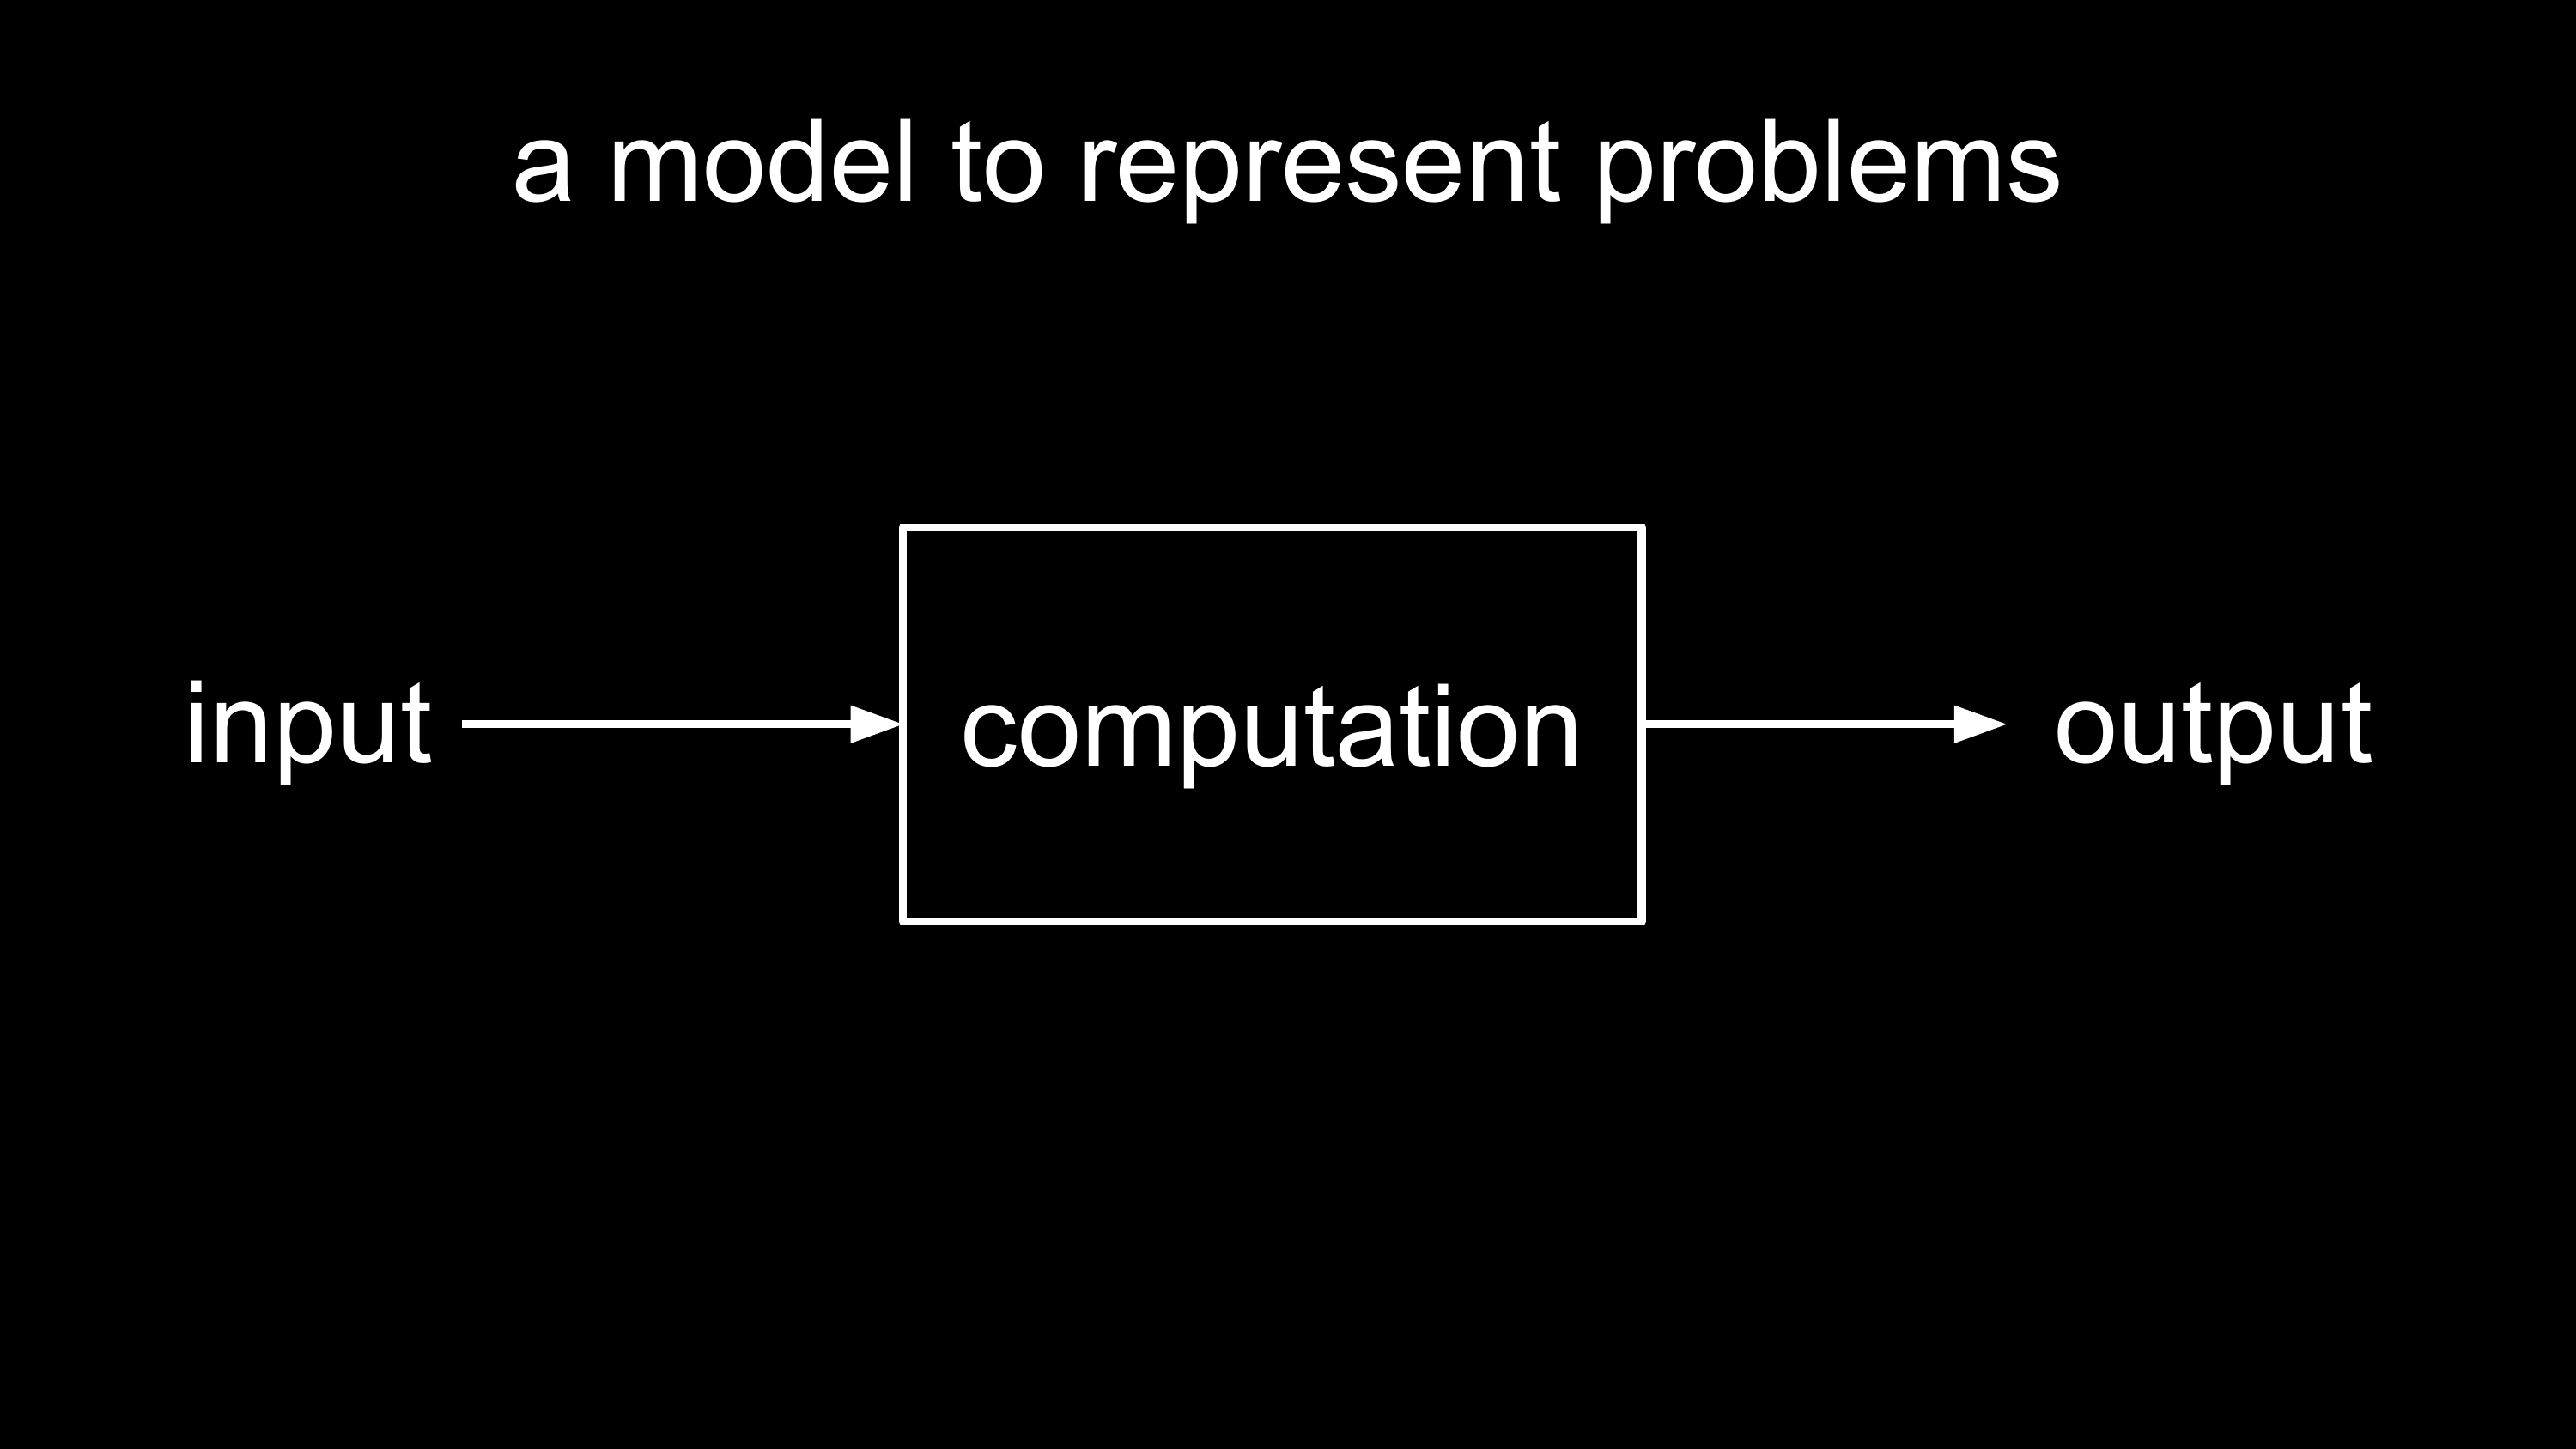
\includegraphics[width=0.6\linewidth,height=\textheight,keepaspectratio]{index_files/mediabag/problem_solving_inpu.png}

}

\caption{\label{fig-input-computation-output}Das EVA-Modell besteht aus
der Eingabe, der Berechnung und der Ausgabe.}

\end{figure}%

Wenden wir das EVA-Modell auf das LiFi-Projekt an. Das LiFi-Gerät soll
verschiedene Daten erfassen: Lichtsignale von einem anderen LiFi-Gerät
und die Temperatur des eigenen Sensors. Basierend auf diesen Daten
trifft es eine Entscheidung. Anschließend kommuniziert es diese
Entscheidung zusammen mit den erfassten Temperaturdaten über
Lichtsignale an das nächste Gerät. Zwar ist jeder dieser Teilschritte
für sich genommen komplex und erfordert eine eigene Lösung. Dennoch
können wir das EVA-Modell nutzen, um das LiFi-Projekt als Ganzes
darzustellen, indem wir von den Details der einzelnen Schritte
abstrahieren:

\begin{center}
\includegraphics[width=0.6\linewidth,height=\textheight,keepaspectratio]{index_files/mediabag/problem_solving_inpu1.png}
\end{center}

Was haben wir nun dadurch gewonnen, dass wir das EVA-Modell angewendet
haben? Wir können uns nun auf die einzelnen Elemente konzentrieren und
diese getrennt voneinander betrachten. Damit zerlegen wir das große,
überfordernde Problem in kleinere Teile und machen es dadurch besser
beherrschbar.

Bei den Eingaben müssen wir uns fragen, wie diese konkret aussehen und
erfasst werden. Dabei geht es vor allem darum, in welcher Form die
Eingaben dem Computer vorliegen müssen, damit er sie verarbeiten kann.
Wie werden Lichtsignale im Computer dargestellt? Wie wird die
physikalische Größe der Umgebungstemperatur in eine
computerverständliche Form umgewandelt, und wie sieht diese aus? Es geht
also um die \textbf{Repräsentation von Informationen}.

Sobald wir die Darstellung der Eingaben geklärt haben, können wir diese
als Grundlage für die Verarbeitung nutzen. Wie muss ein Programm
aussehen, das auf Basis der Eingabedaten die richtige Entscheidung
trifft? Welche Schritte sind notwendig? Welche Prüfungen muss das
Programm durchführen? Bei diesem Schritt geht es folglich um die
\textbf{Verarbeitung von Informationen}.

Schließlich müssen wir die Form der Ausgabe festlegen. Wie soll das
Verarbeitungsergebnis konkret aussehen? Da wir für die Kommunikation
wieder Lichtsignale verwenden, geht es auch bei der Ausgabe um die
\textbf{Repräsentation von Informationen}.

Wir können die Perspektive auf eine geräteübergreifende LiFi-Sicht
erweitern. Dann kommt neben der Repräsentation von Informationen ein
weiterer Aspekt hinzu: Die \textbf{Kommunikation von Informationen}. Wie
übertragen wir die Informationen vom ersten LiFi-Gerät zum nächsten?

\begin{center}
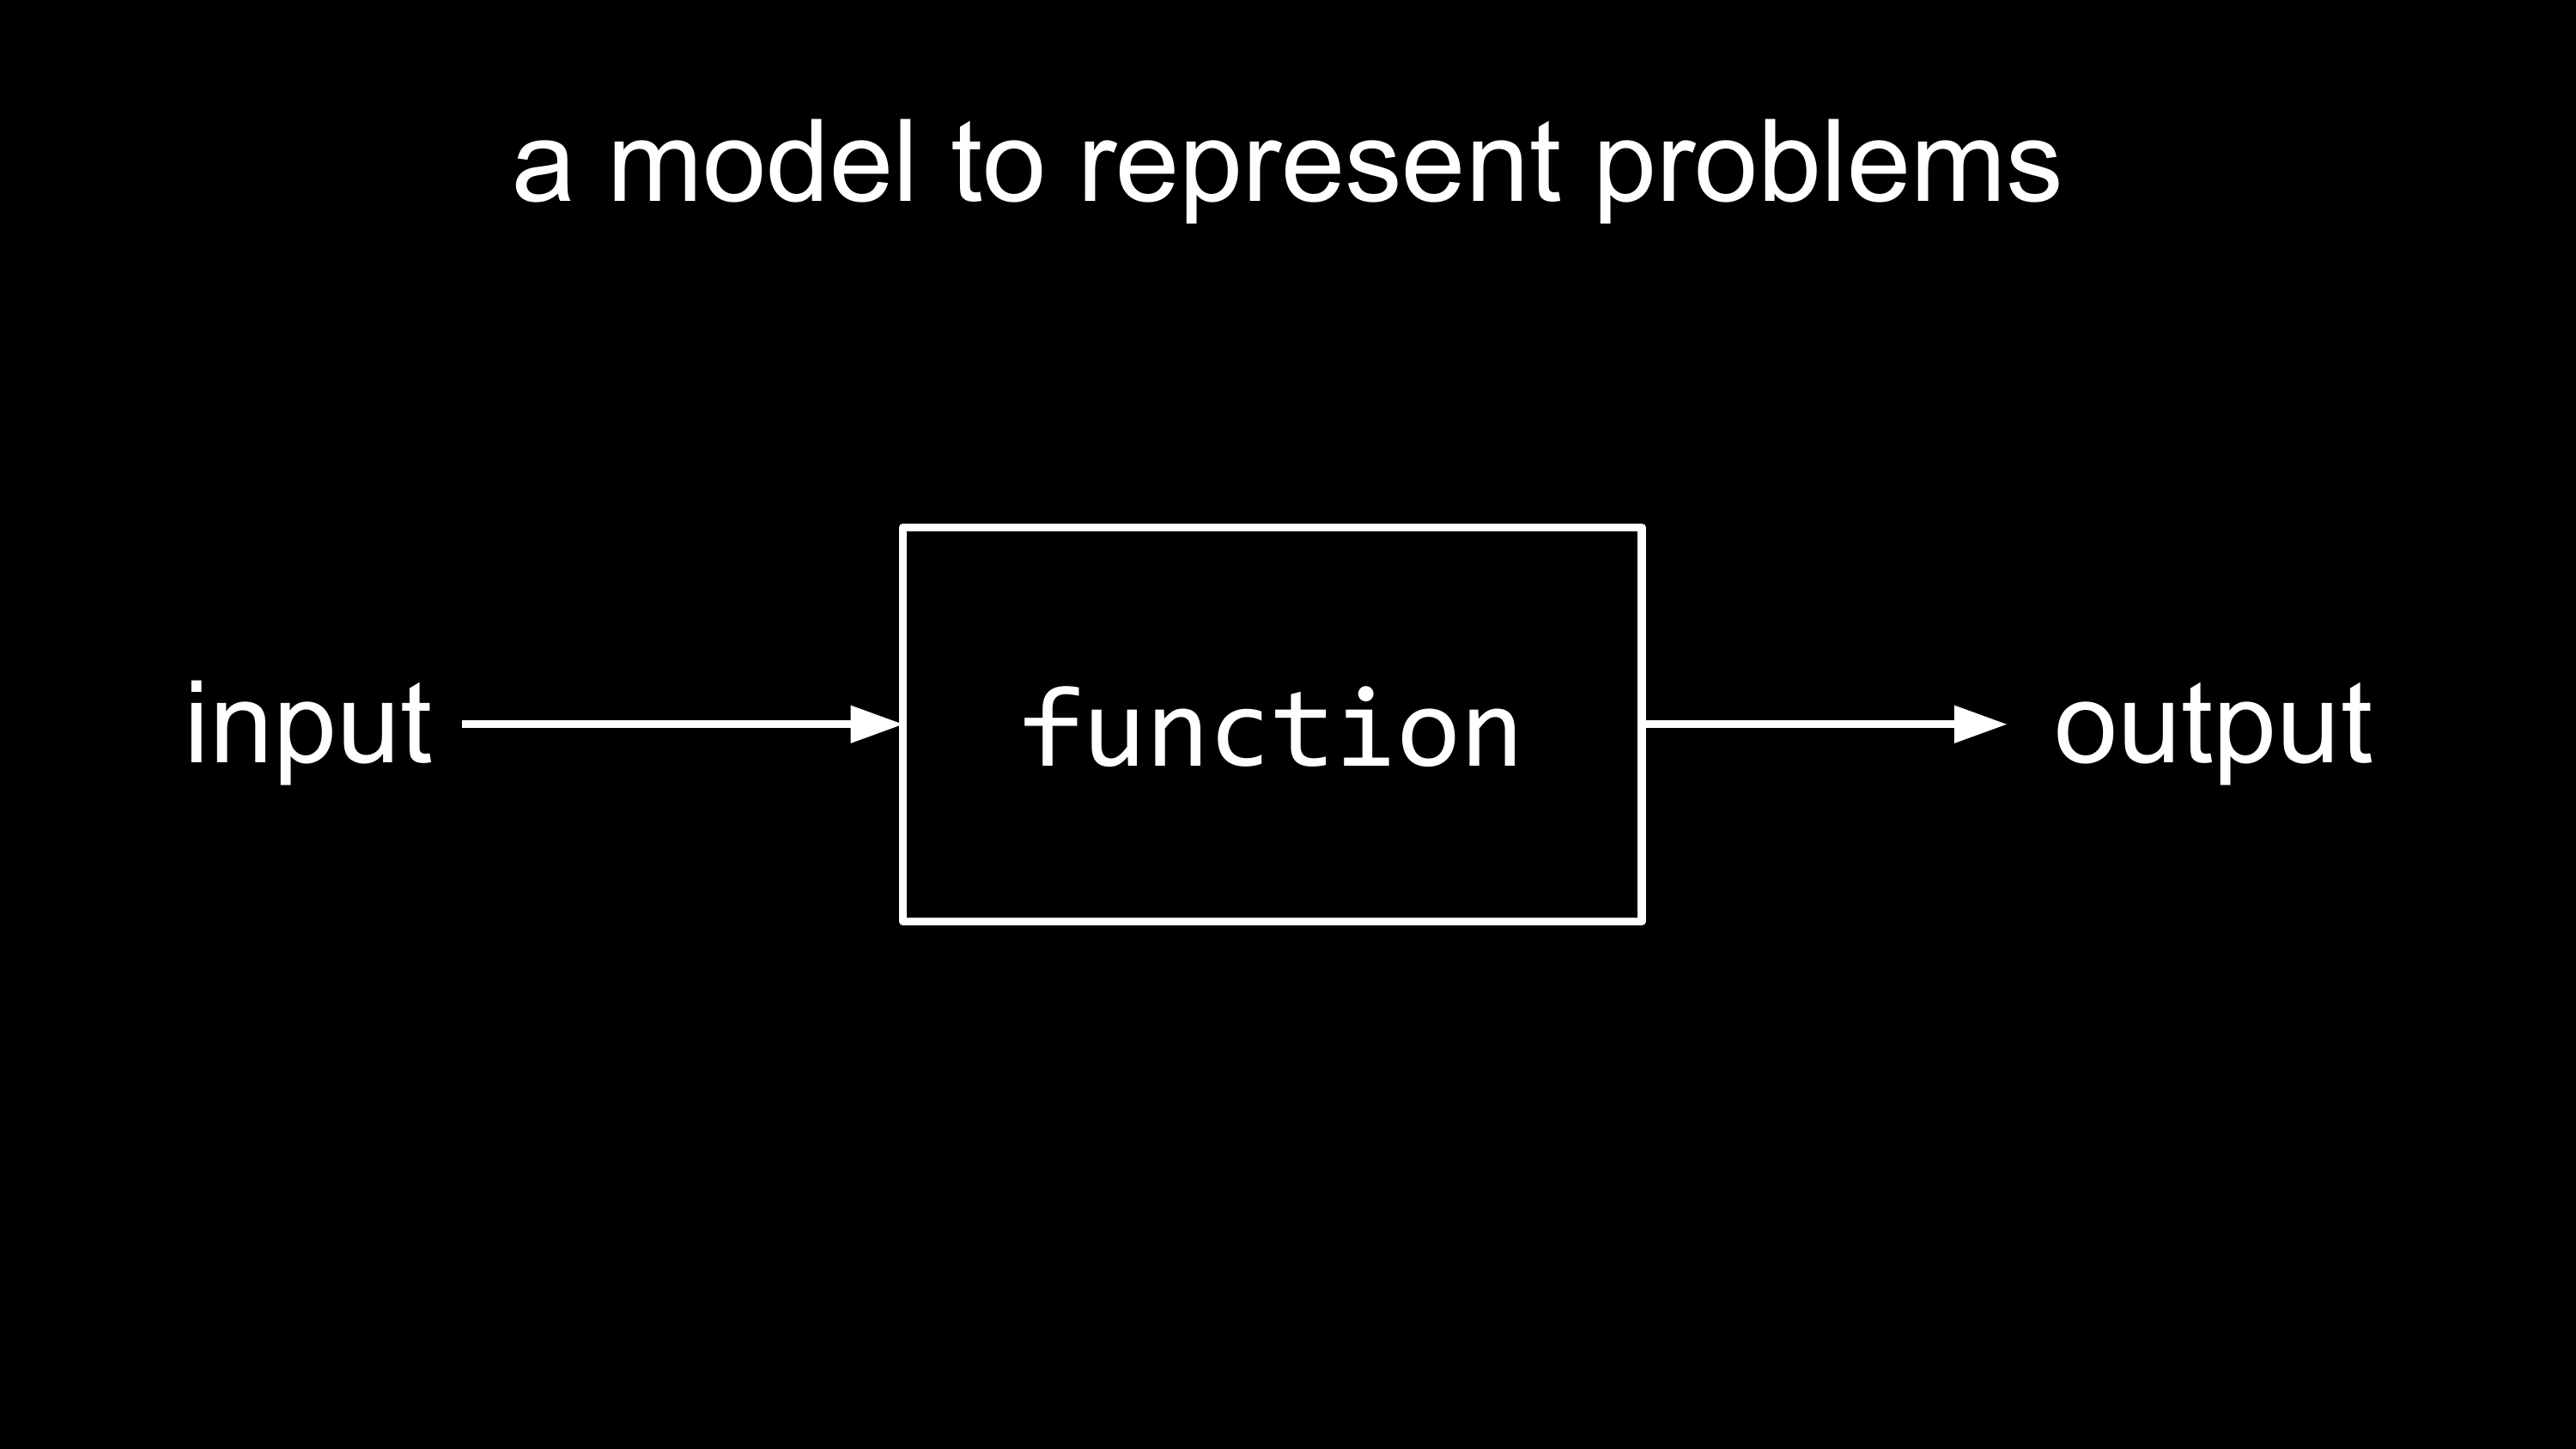
\includegraphics[width=0.6\linewidth,height=\textheight,keepaspectratio]{index_files/mediabag/problem_solving_inpu12.png}
\end{center}

Vielleicht ist dir aufgefallen, dass die Struktur des gesamten Buches an
den gerade identifizierten, übergeordneten Problemstellungen
ausgerichtet ist. Wir befinden uns gerade im
\href{part-problems.qmd}{ersten Teil} und sprechen darüber, wie wir
Probleme im Computer darstellen. Im
\href{part-representation.qmd}{zweiten Teil des Buches} lernen wir, wie
Computer ganz unterschiedliche Informationen repräsentieren können,
damit sie für die Lösung des Problems verwendet werden können. Im
\href{part-processing.qmd}{dritten Teil} beschäftigen wir uns damit, wie
Computer Informationen verarbeiten. Der
\href{part-communication.qmd}{vierte und letzte Teil} führt uns in
wichtige Konzepte der Kommunikation mittels Computern und Netzwerken
ein.

\subsubsection{Beispiel: Taschenrechner}\label{beispiel-taschenrechner}

Am Beispiel eines Taschenrechner lässt sich das EVA-Modell gut
darstellen. Wir können uns bildlich vorstellen, wie ein Mensch die
Eingabe tätigt und danach das Ergebnis abliest. Es ist wichtig zu
verstehen, dass Eingabe und Ausgabe sehr unterschiedliche Formen
annehmen können und keinesfalls nur über eine Tastatur erfolgen müssen.

Das Beispiel des Taschenrechners wird in
Abbildung~\ref{fig-example-calculator} anhand einer einfachen Addition
zweier Zahlen konkreter verdeutlicht. Als Eingabe werden zwei Zahlen
benötigt, die Berechnung erfolgt durch eine Addition, dargestellt durch
das Plussymbol. Die Ausgabe ist das Ergebnis -- die Summe.

\begin{figure}

\centering{

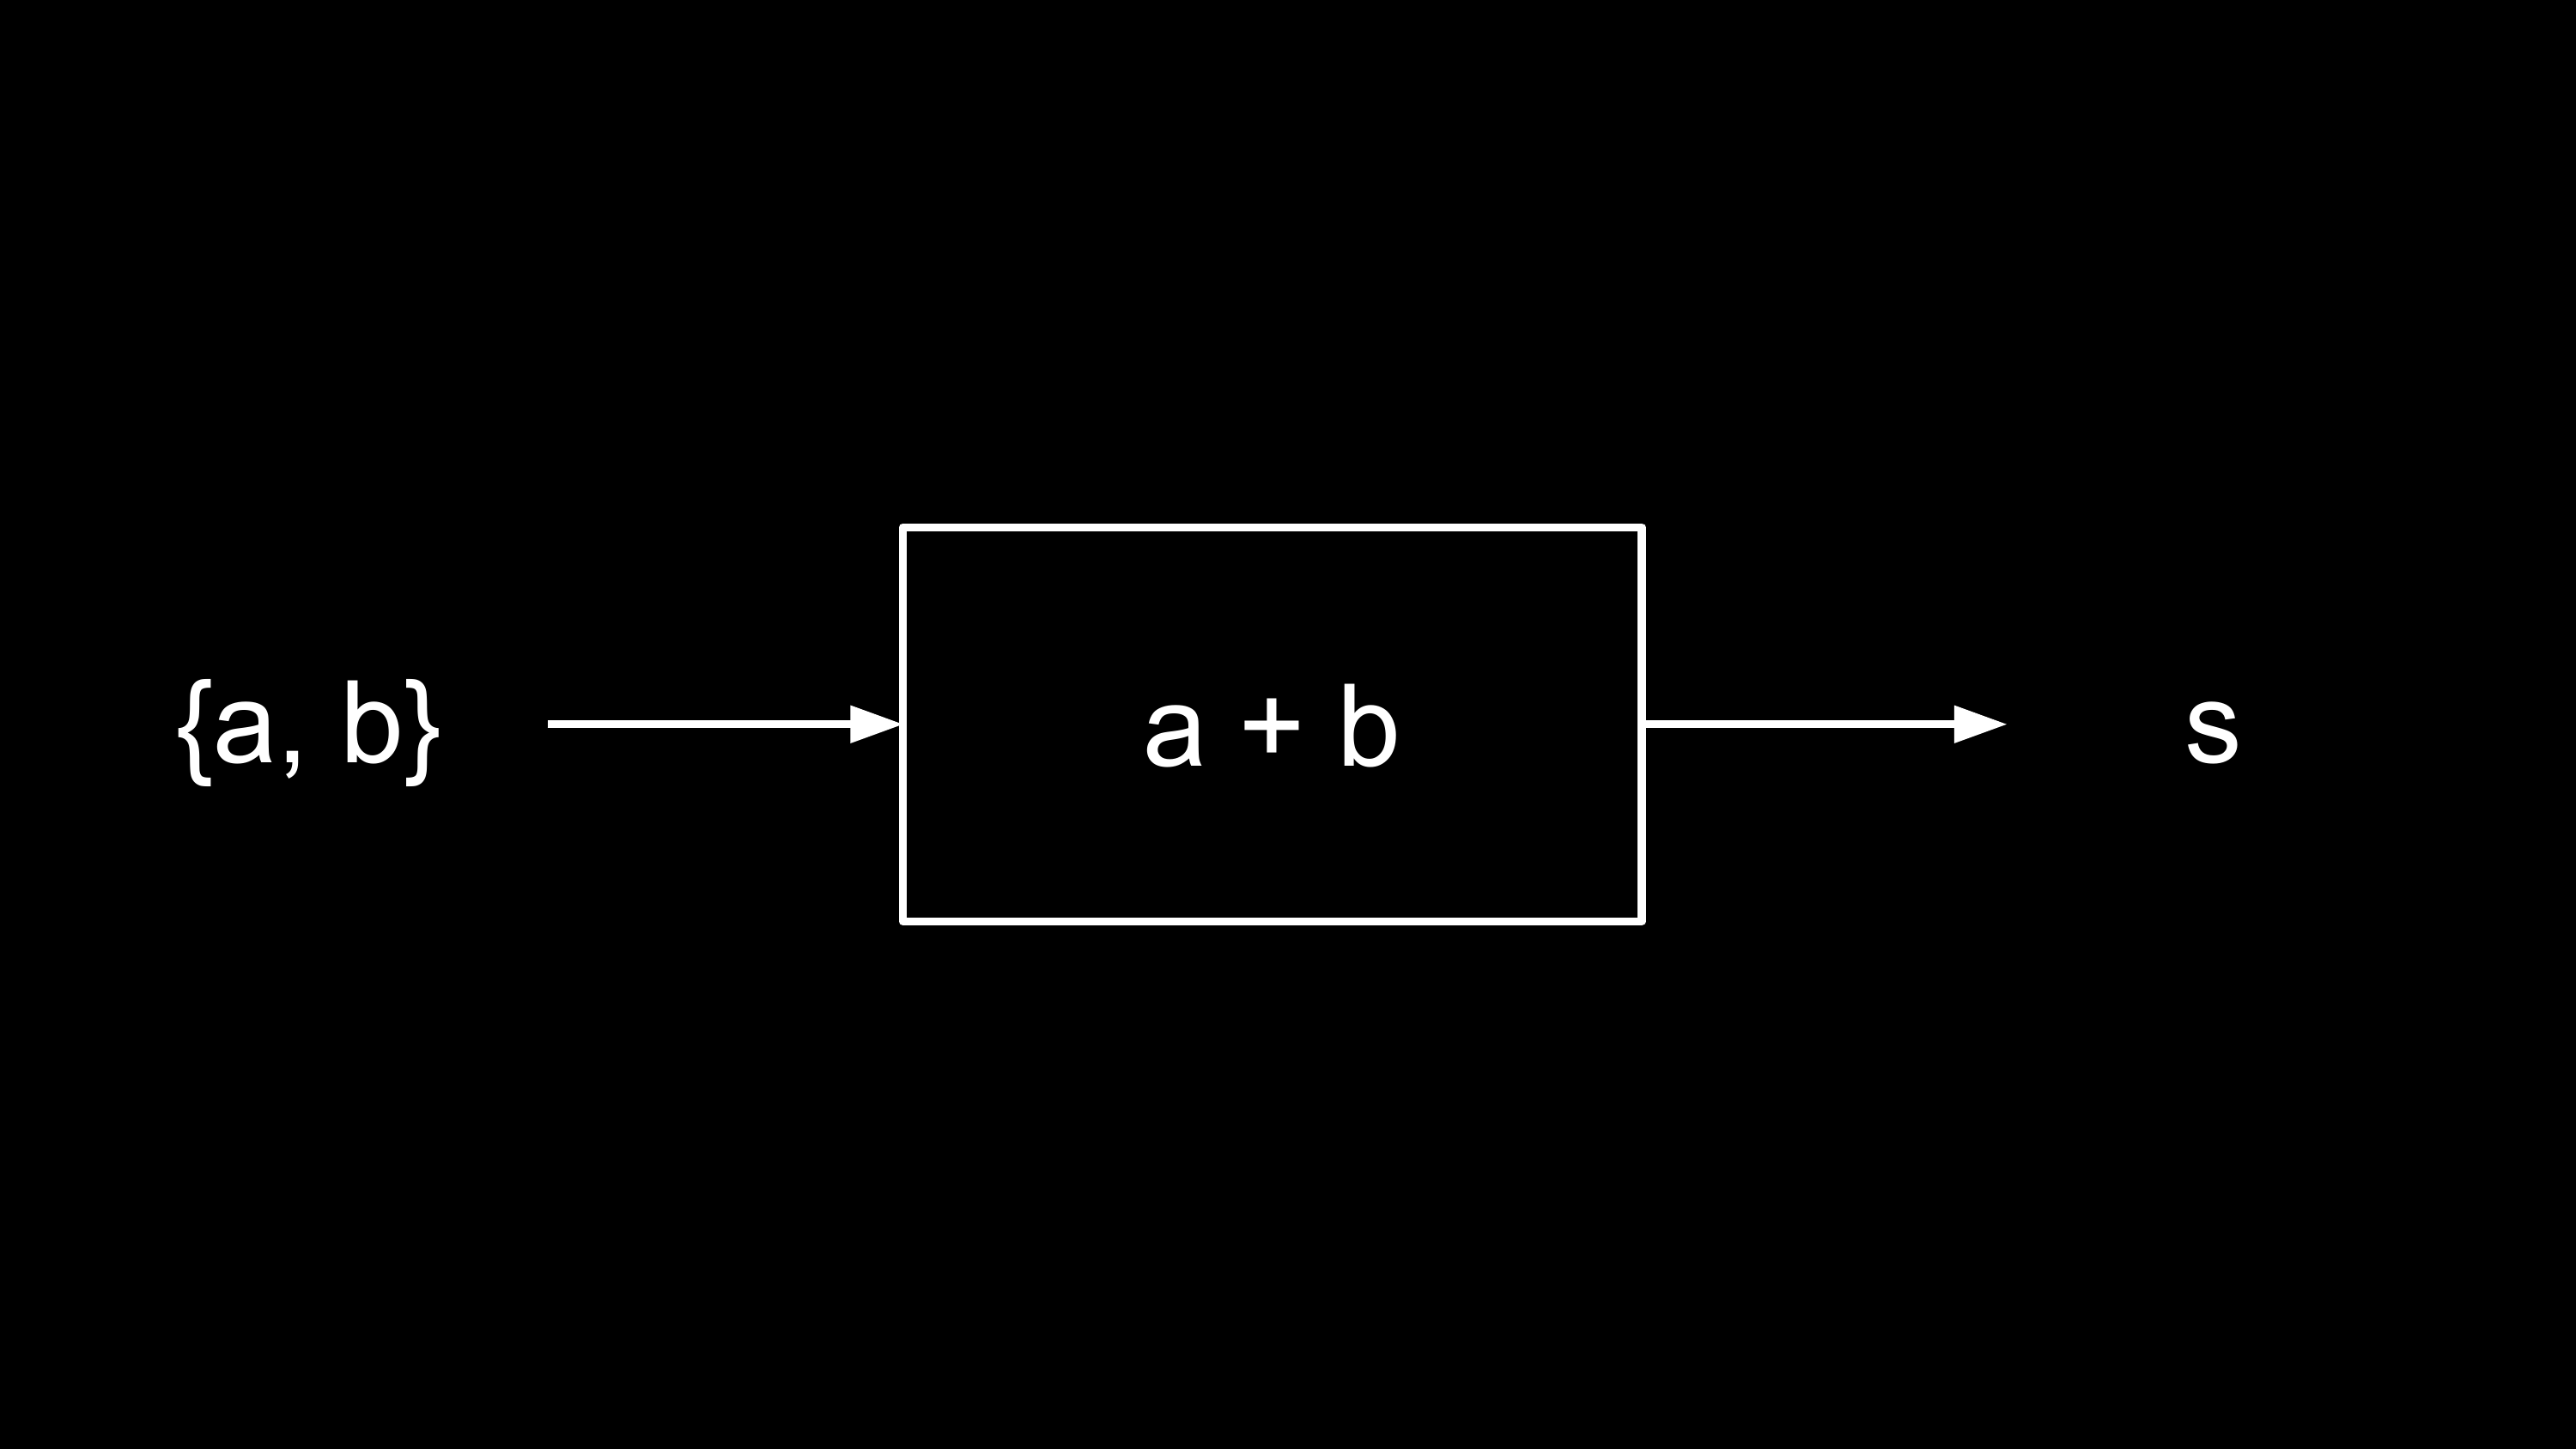
\includegraphics[width=0.6\linewidth,height=\textheight,keepaspectratio]{index_files/mediabag/problem_solving_exam.png}

}

\caption{\label{fig-example-calculator}Das EVA-Modell für die Addition
zweier Zahlen.}

\end{figure}%

Dieses einfache Beispiel zeigt, dass wir verstehen müssen, wie Computer
die drei Bestandteile des EVA-Modells umsetzen. Beim Taschenrechner sind
Ein- und Ausgabe jeweils Zahlen. Diese Daten speichert der Computer in
seinem Arbeitsspeicher. Dabei ist wichtig zu wissen, dass Computer auf
der untersten Ebene ausschließlich Nullen und Einsen speichern. Wir
müssen also verstehen, wie Computer Zahlen mithilfe dieser Binärzahlen
darstellen können.

Was passiert bei der Berechnung in der Mitte des Modells? Eine Addition
mag uns einfach erscheinen, doch auch hier müssen wir beachten, dass
Computer mit Binärzahlen arbeiten. Es stellt sich also die Frage: Wie
funktioniert eine Addition, wenn die Zahlen als Folge von Nullen und
Einsen dargestellt sind? Auf die beiden Fragen zur
\textbf{Repräsentation und der Verarbeitung von Informationen} im
binären System werden wir im Laufe des Buches Antworten bekommen.

\subsubsection{Beispiel: Pflanzen
zählen}\label{beispiel-pflanzen-zuxe4hlen}

Betrachten wir ein weiteres Beispiel: Stell dir vor, du möchtest einen
Computer nutzen, um Maispflanzen auf einer Drohnenaufnahme eines Ackers
zu zählen. Diese Aufgabe ist für Menschen zwar einfach zu verstehen,
wäre aber sehr zeitaufwändig auszuführen. Moderne Algorithmen
ermöglichen es Computern, Objekte auf Bildern präzise zu lokalisieren
und zu zählen. Nehmen wir an, wir haben für dieses Problem bereits eine
Lösung entwickelt und ein Programm namens \texttt{count\_plants}
erstellt. Nun stellt sich die Frage: Wie sehen die Eingabe und die
Ausgabe für dieses Problem aus? Was benötigt das Programm von uns, und
was liefert es als Ergebnis?

\begin{center}
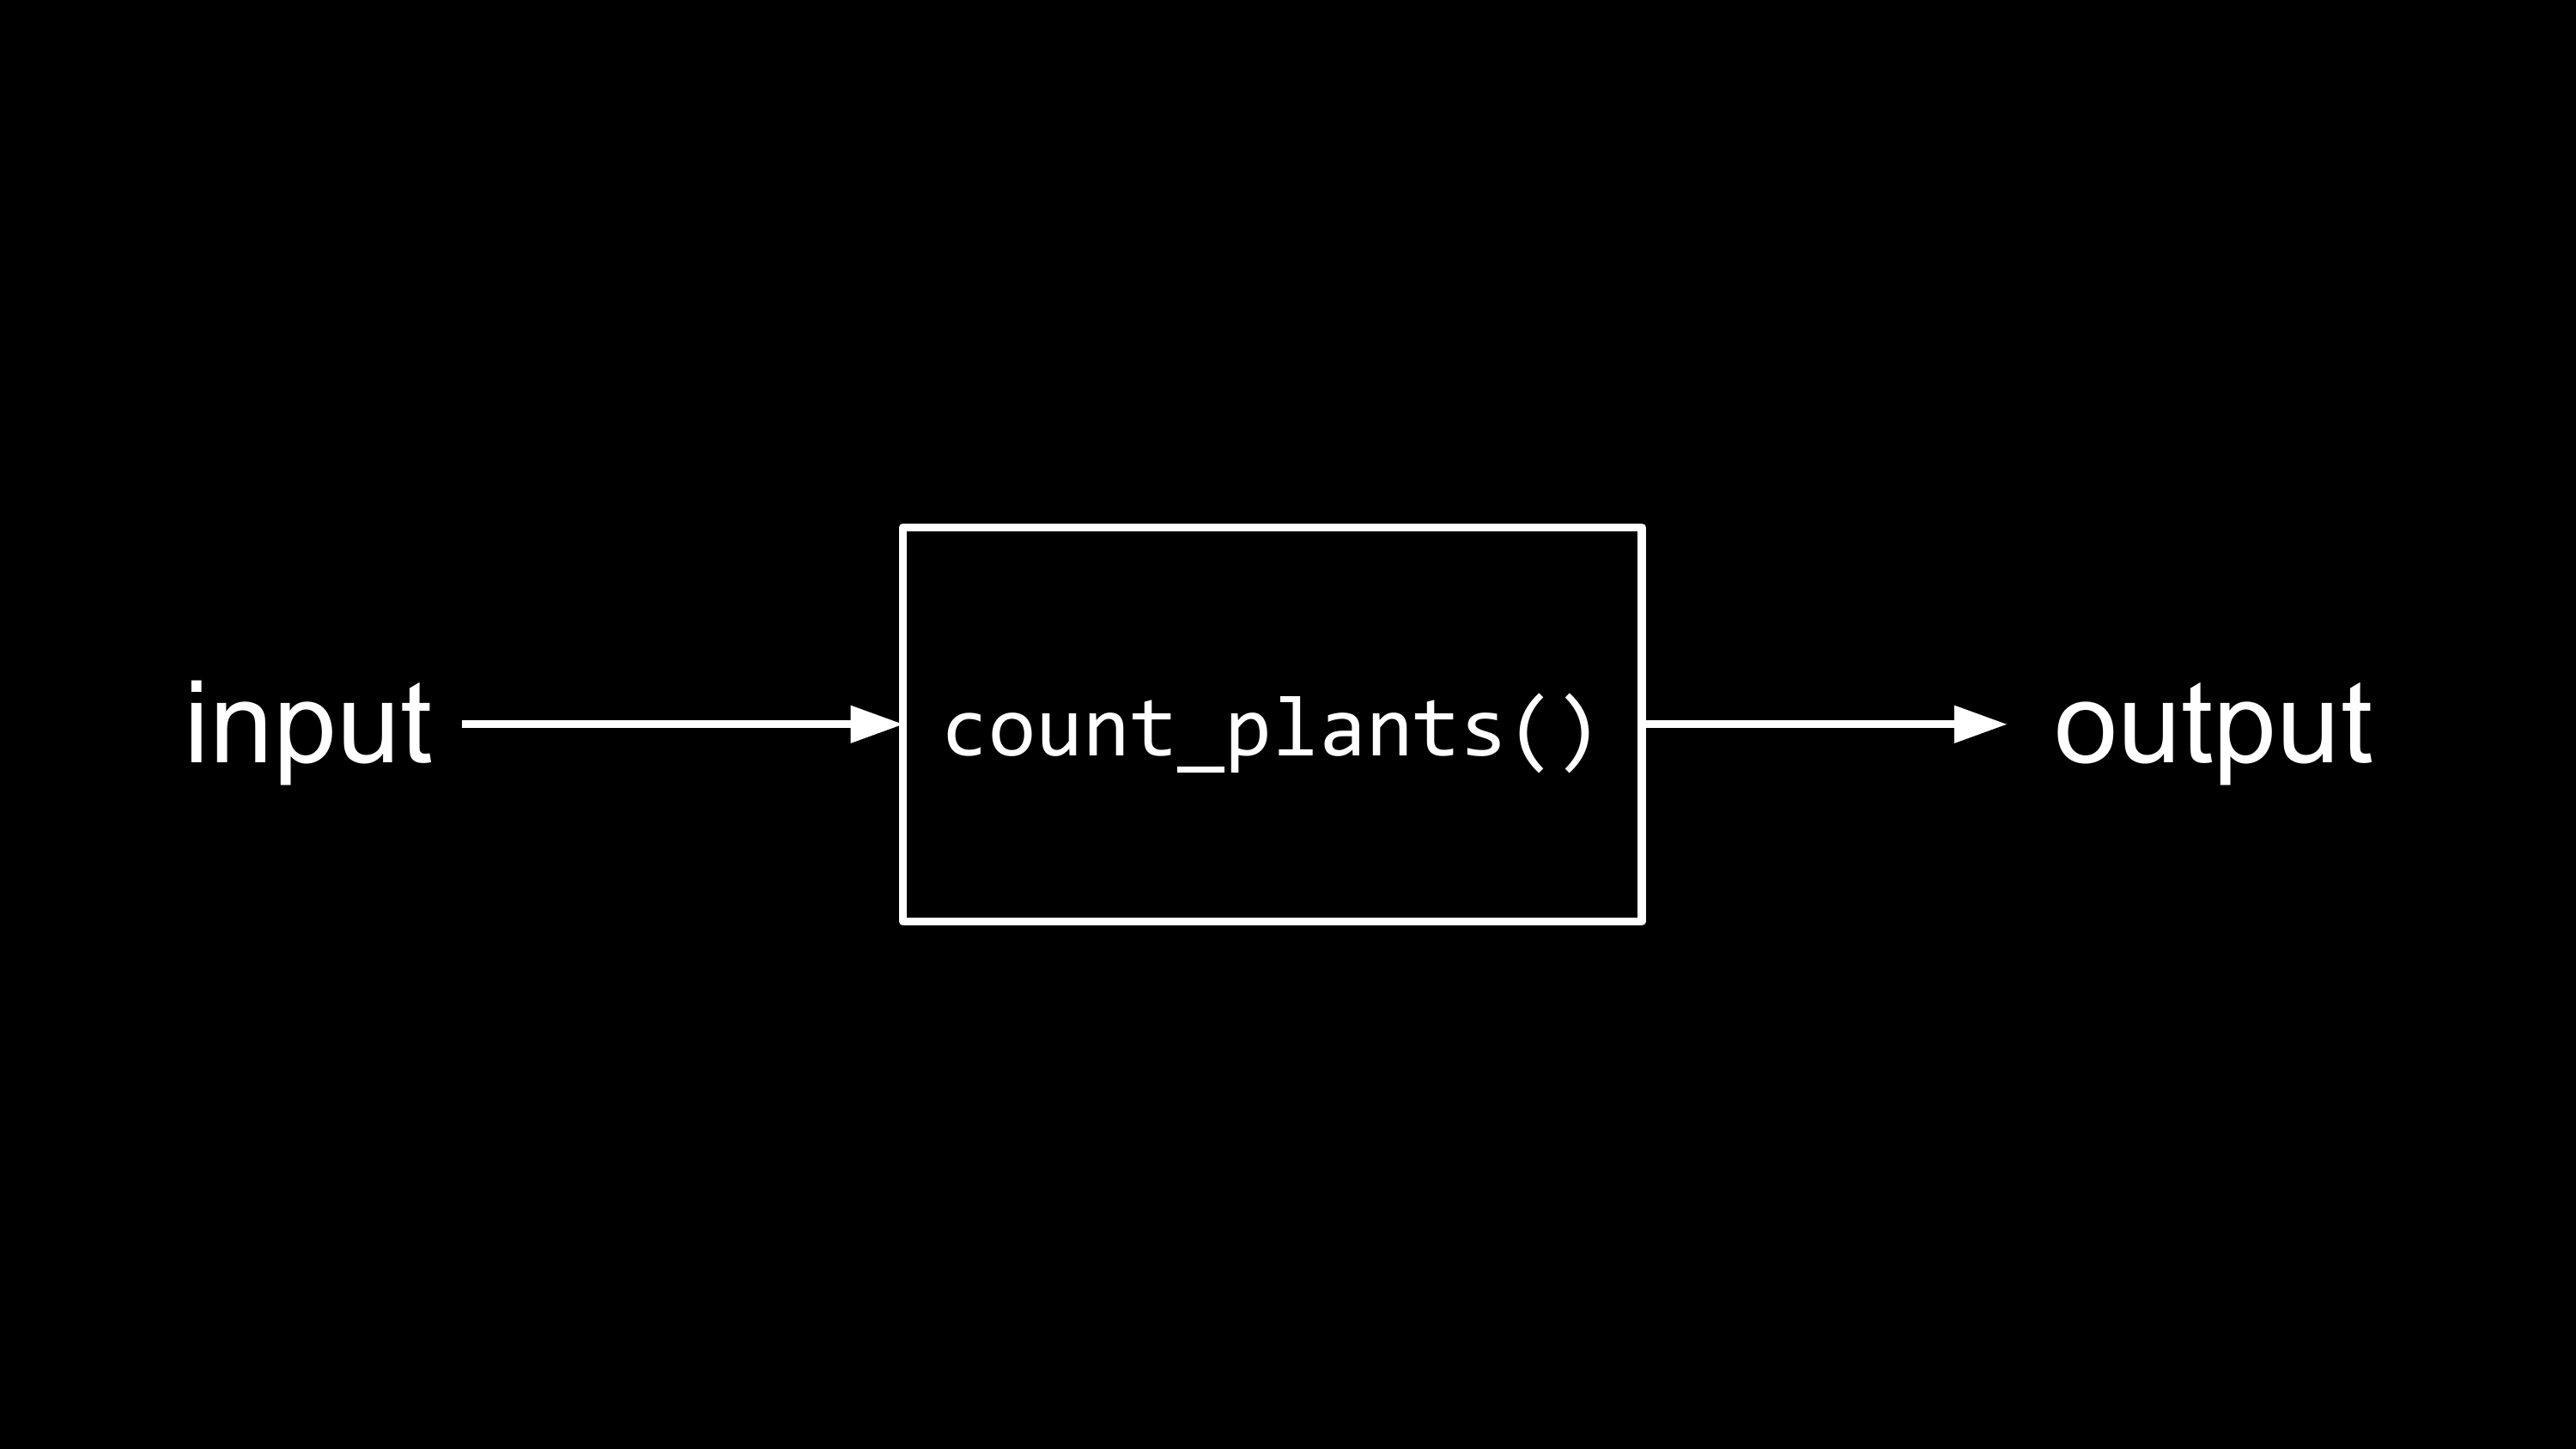
\includegraphics[width=0.6\linewidth,height=\textheight,keepaspectratio]{index_files/mediabag/problem_solving_exam1.png}
\end{center}

Die erwartete \textbf{Ausgabe} lässt sich einfach beschreiben: Das
Ergebnis der Zählung ist eine ganze Zahl. Die \textbf{Eingabe} für
dieses Problem ist - anders als beim Taschenrechner - kein Tastendruck,
sondern ein Bild. Damit der Computer das Bild verarbeiten kann, muss es
dem Computer in digitaler Form bereitgestellt werden. Was das genau
bedeutet, lernen wir in einem späteren Kapitel. Hier genügt es uns zu
verstehen, \emph{dass }wir das Bild digital abbilden müssen.

\begin{center}
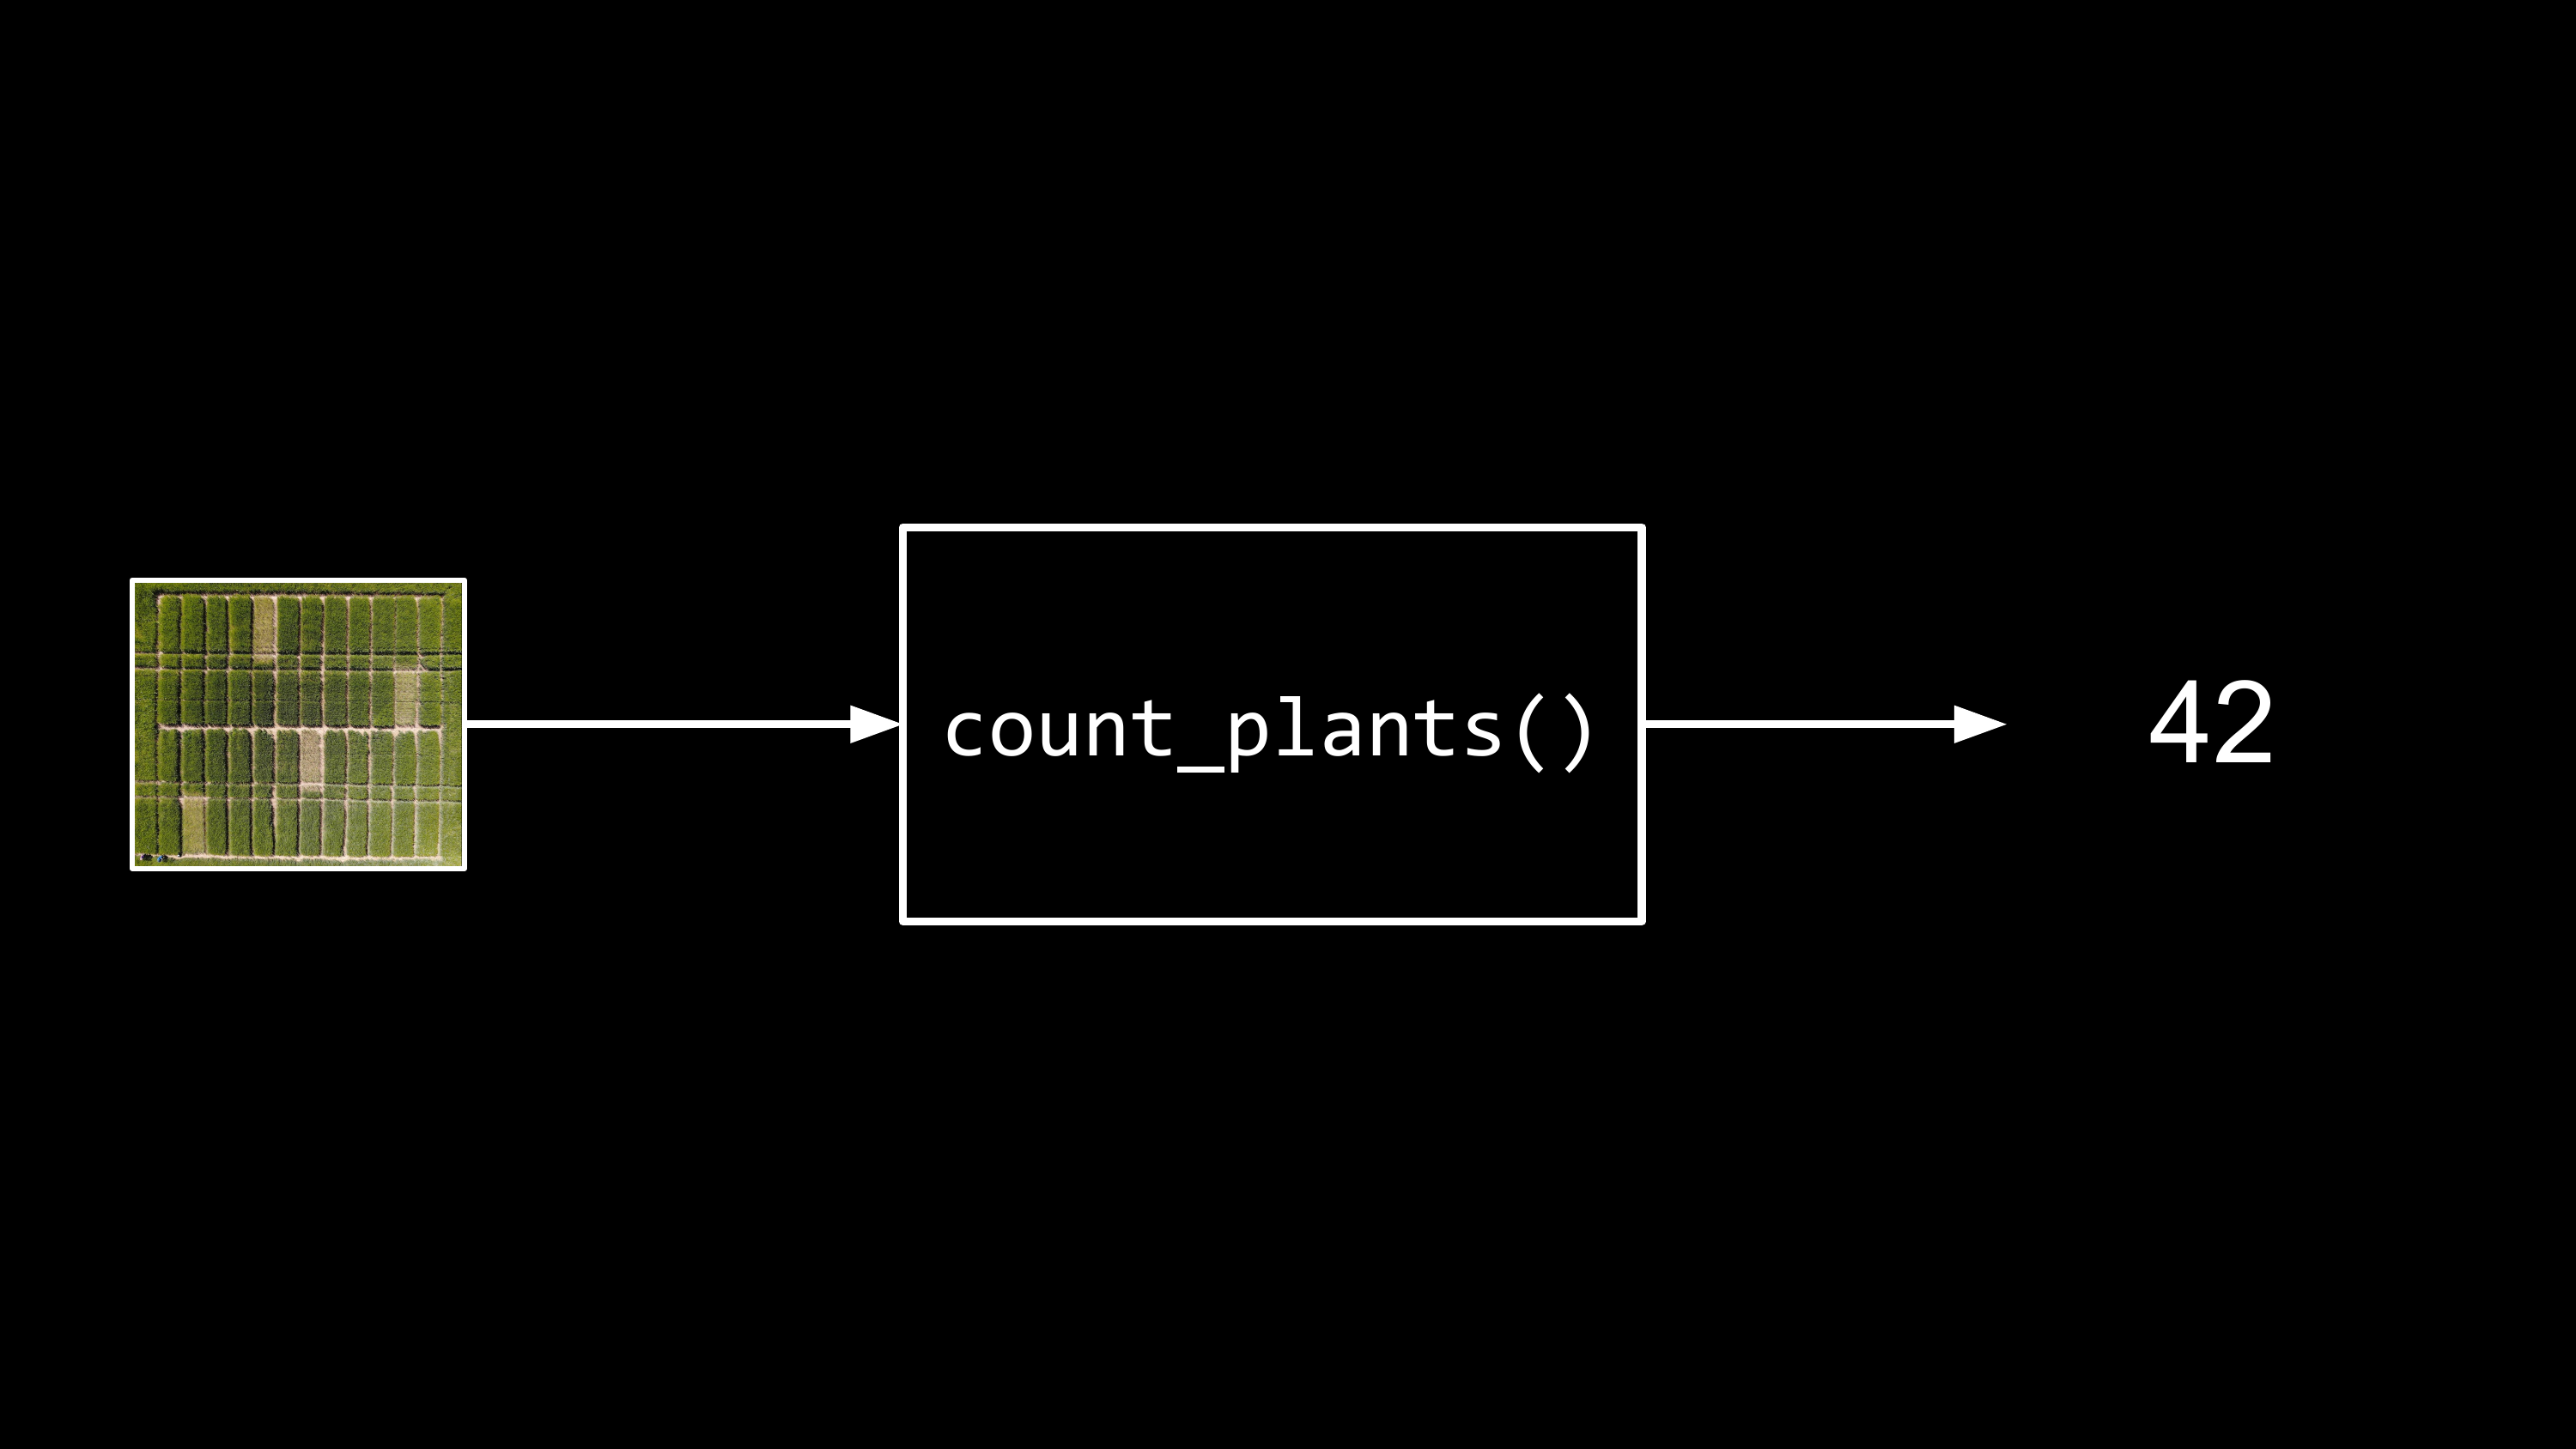
\includegraphics[width=0.6\linewidth,height=\textheight,keepaspectratio]{index_files/mediabag/problem_solving_exam12.png}
\end{center}

Wie gelangt das Bild in den Computer? Dies ist im Modell nicht näher
definiert und für die Problembeschreibung auch nicht wesentlich. Das
Bild muss lediglich irgendwie in den Arbeitsspeicher des Programms
\texttt{count\_plants} gelangen. Dies kann auf verschiedene Arten
geschehen: Es kann von der Festplatte gelesen werden, über eine
drahtlose Verbindung wie Bluetooth direkt übertragen und verarbeitet
werden, oder das Programm \texttt{count\_plants} läuft direkt auf der
Drohne und greift unmittelbar auf deren Kamera zu. Die technische
Umsetzung ist für unser Modell zunächst irrelevant. In einem späteren
Kapitel werden wir uns damit befassen, wie Informationen genau
übertragen und gespeichert werden. Genauso werden wir lernen, wie die
benötigten Informationen für die Ein- und Ausgabe eines Programms in
digitaler Form dargestellt werden können.

\begin{center}
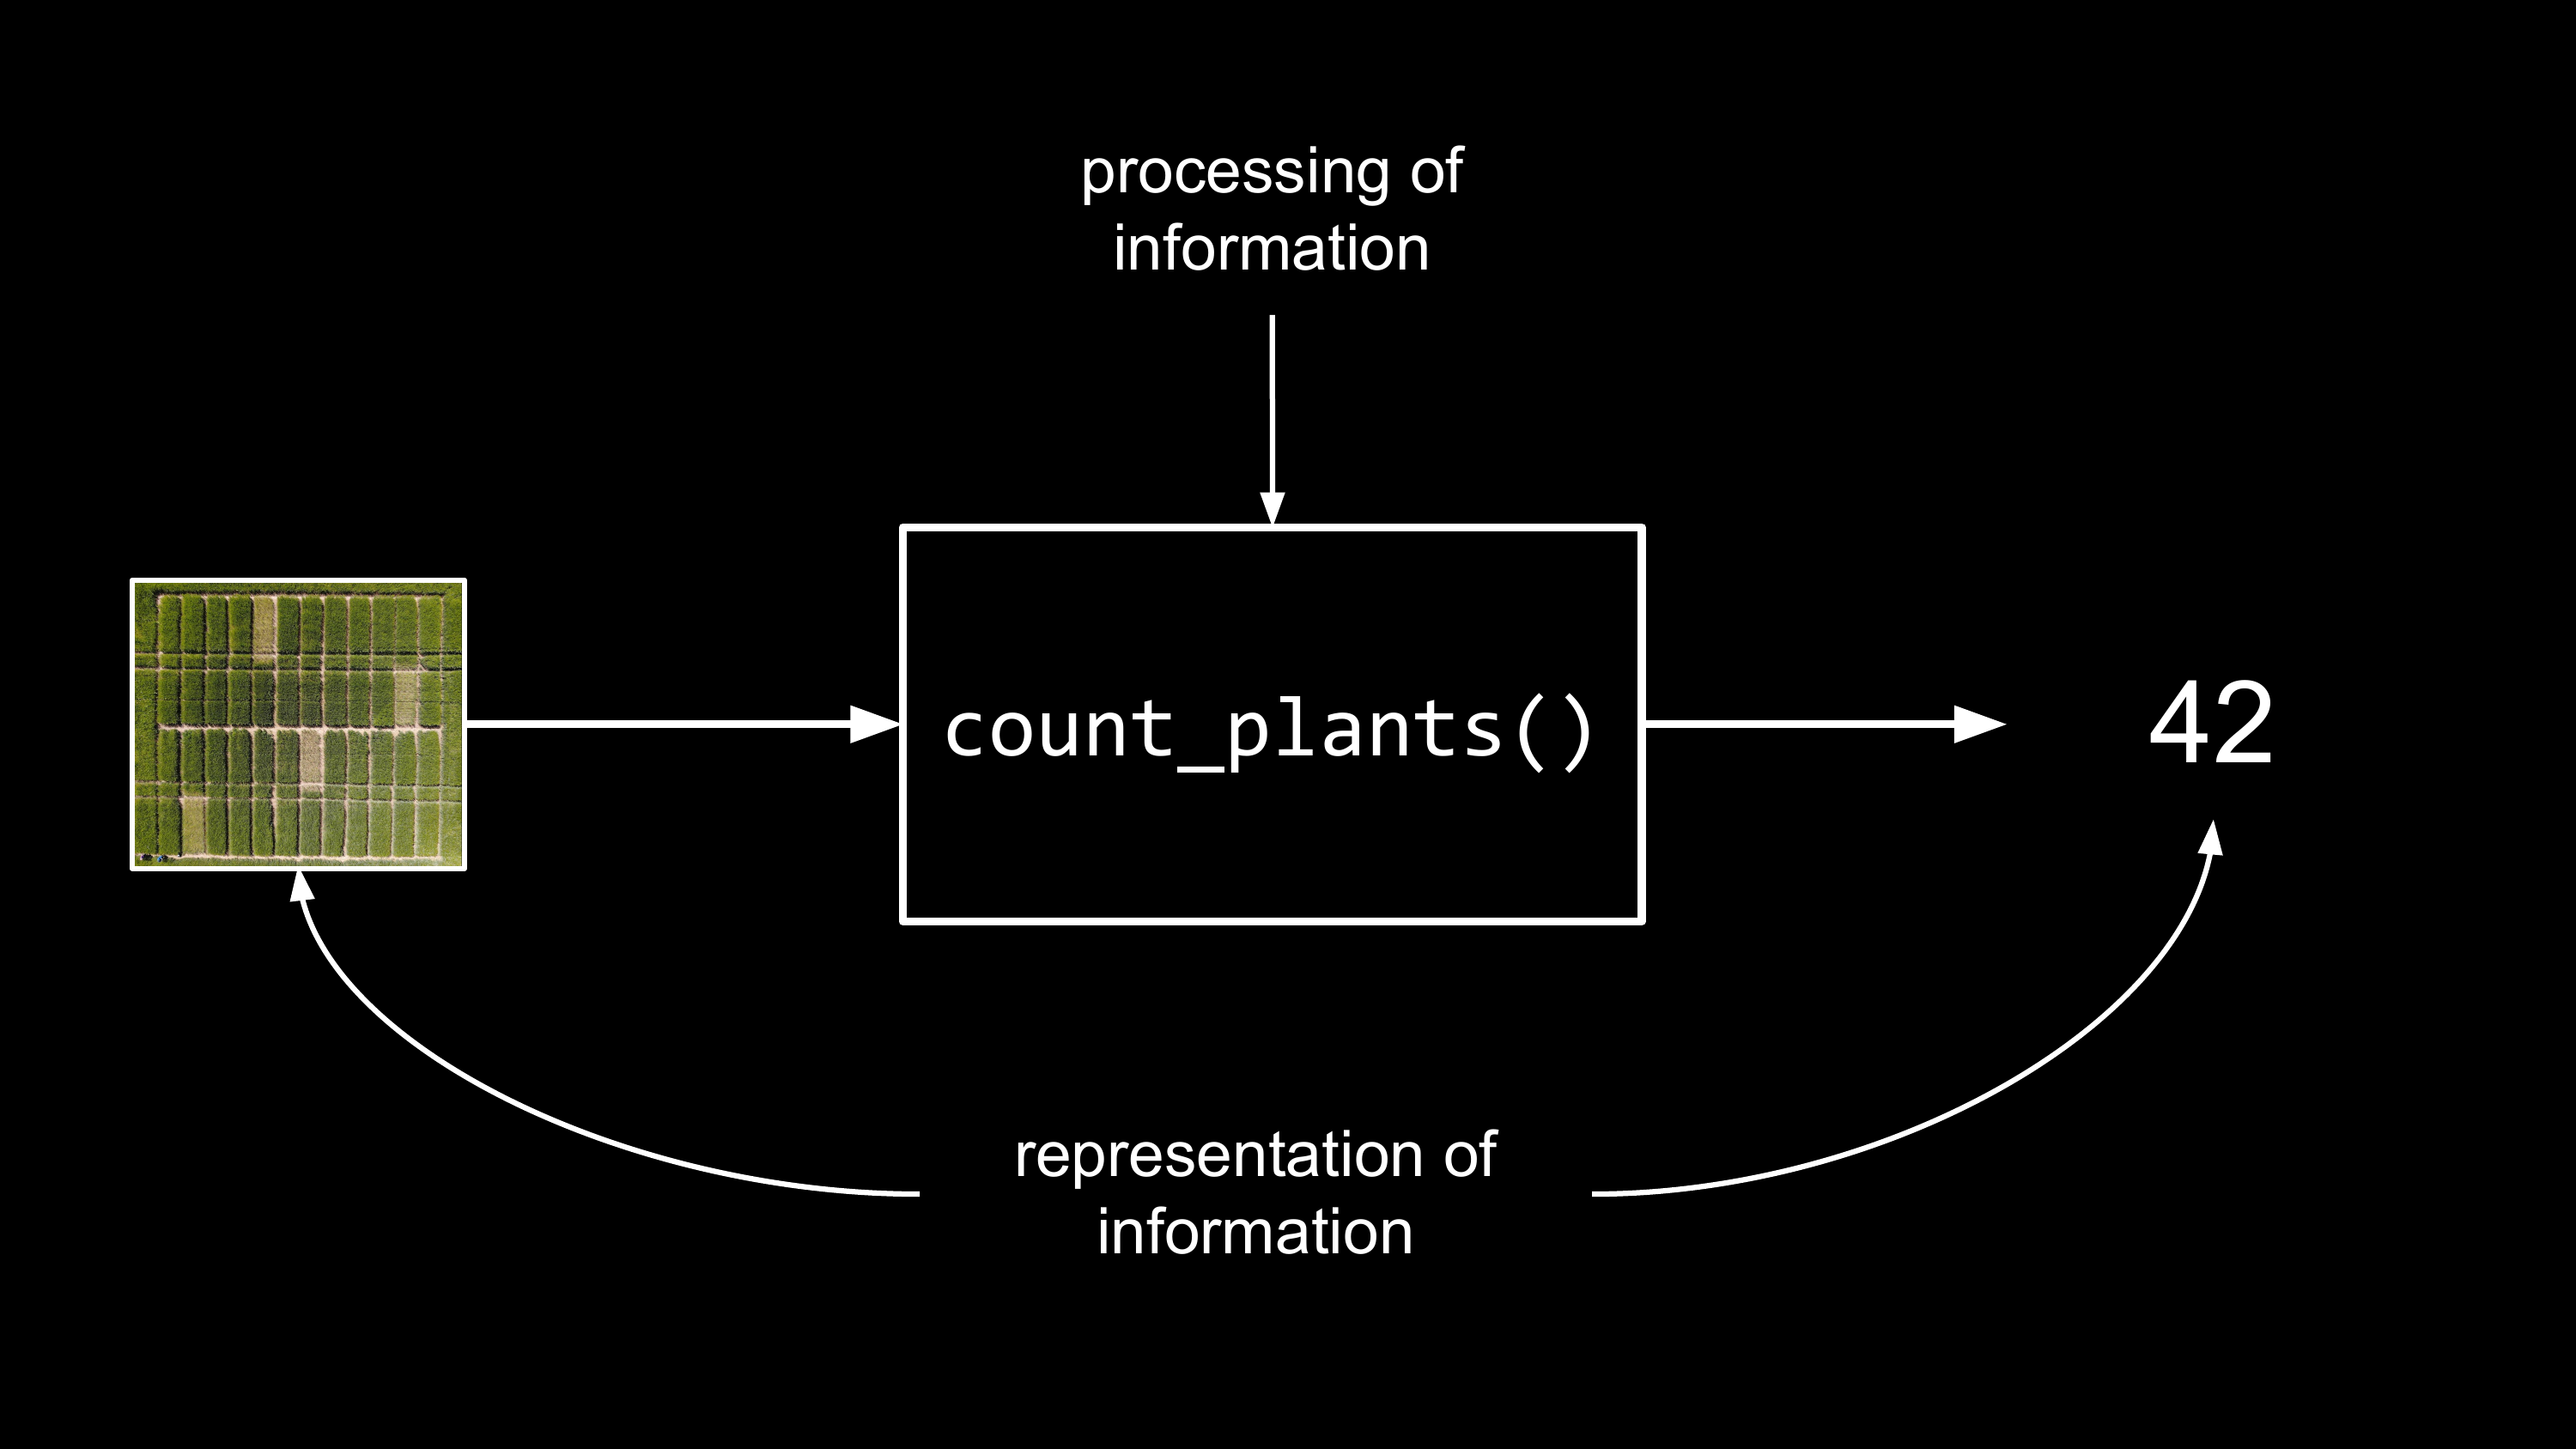
\includegraphics[width=0.6\linewidth,height=\textheight,keepaspectratio]{index_files/mediabag/problem_solving_exam123.png}
\end{center}

\subsubsection{Beispiel: Schach spielen}\label{beispiel-schach-spielen}

Ein weiteres Beispiel zur Verdeutlichung des EVA-Modells ist das
Schachspiel. Das Problem lässt sich einfach beschreiben: Der Computer
soll auf Grundlage einer bestehenden Spielsituation den bestmöglichen
nächsten Zug vorschlagen. Dieser Zug soll die Gewinnchancen maximieren.

\begin{center}
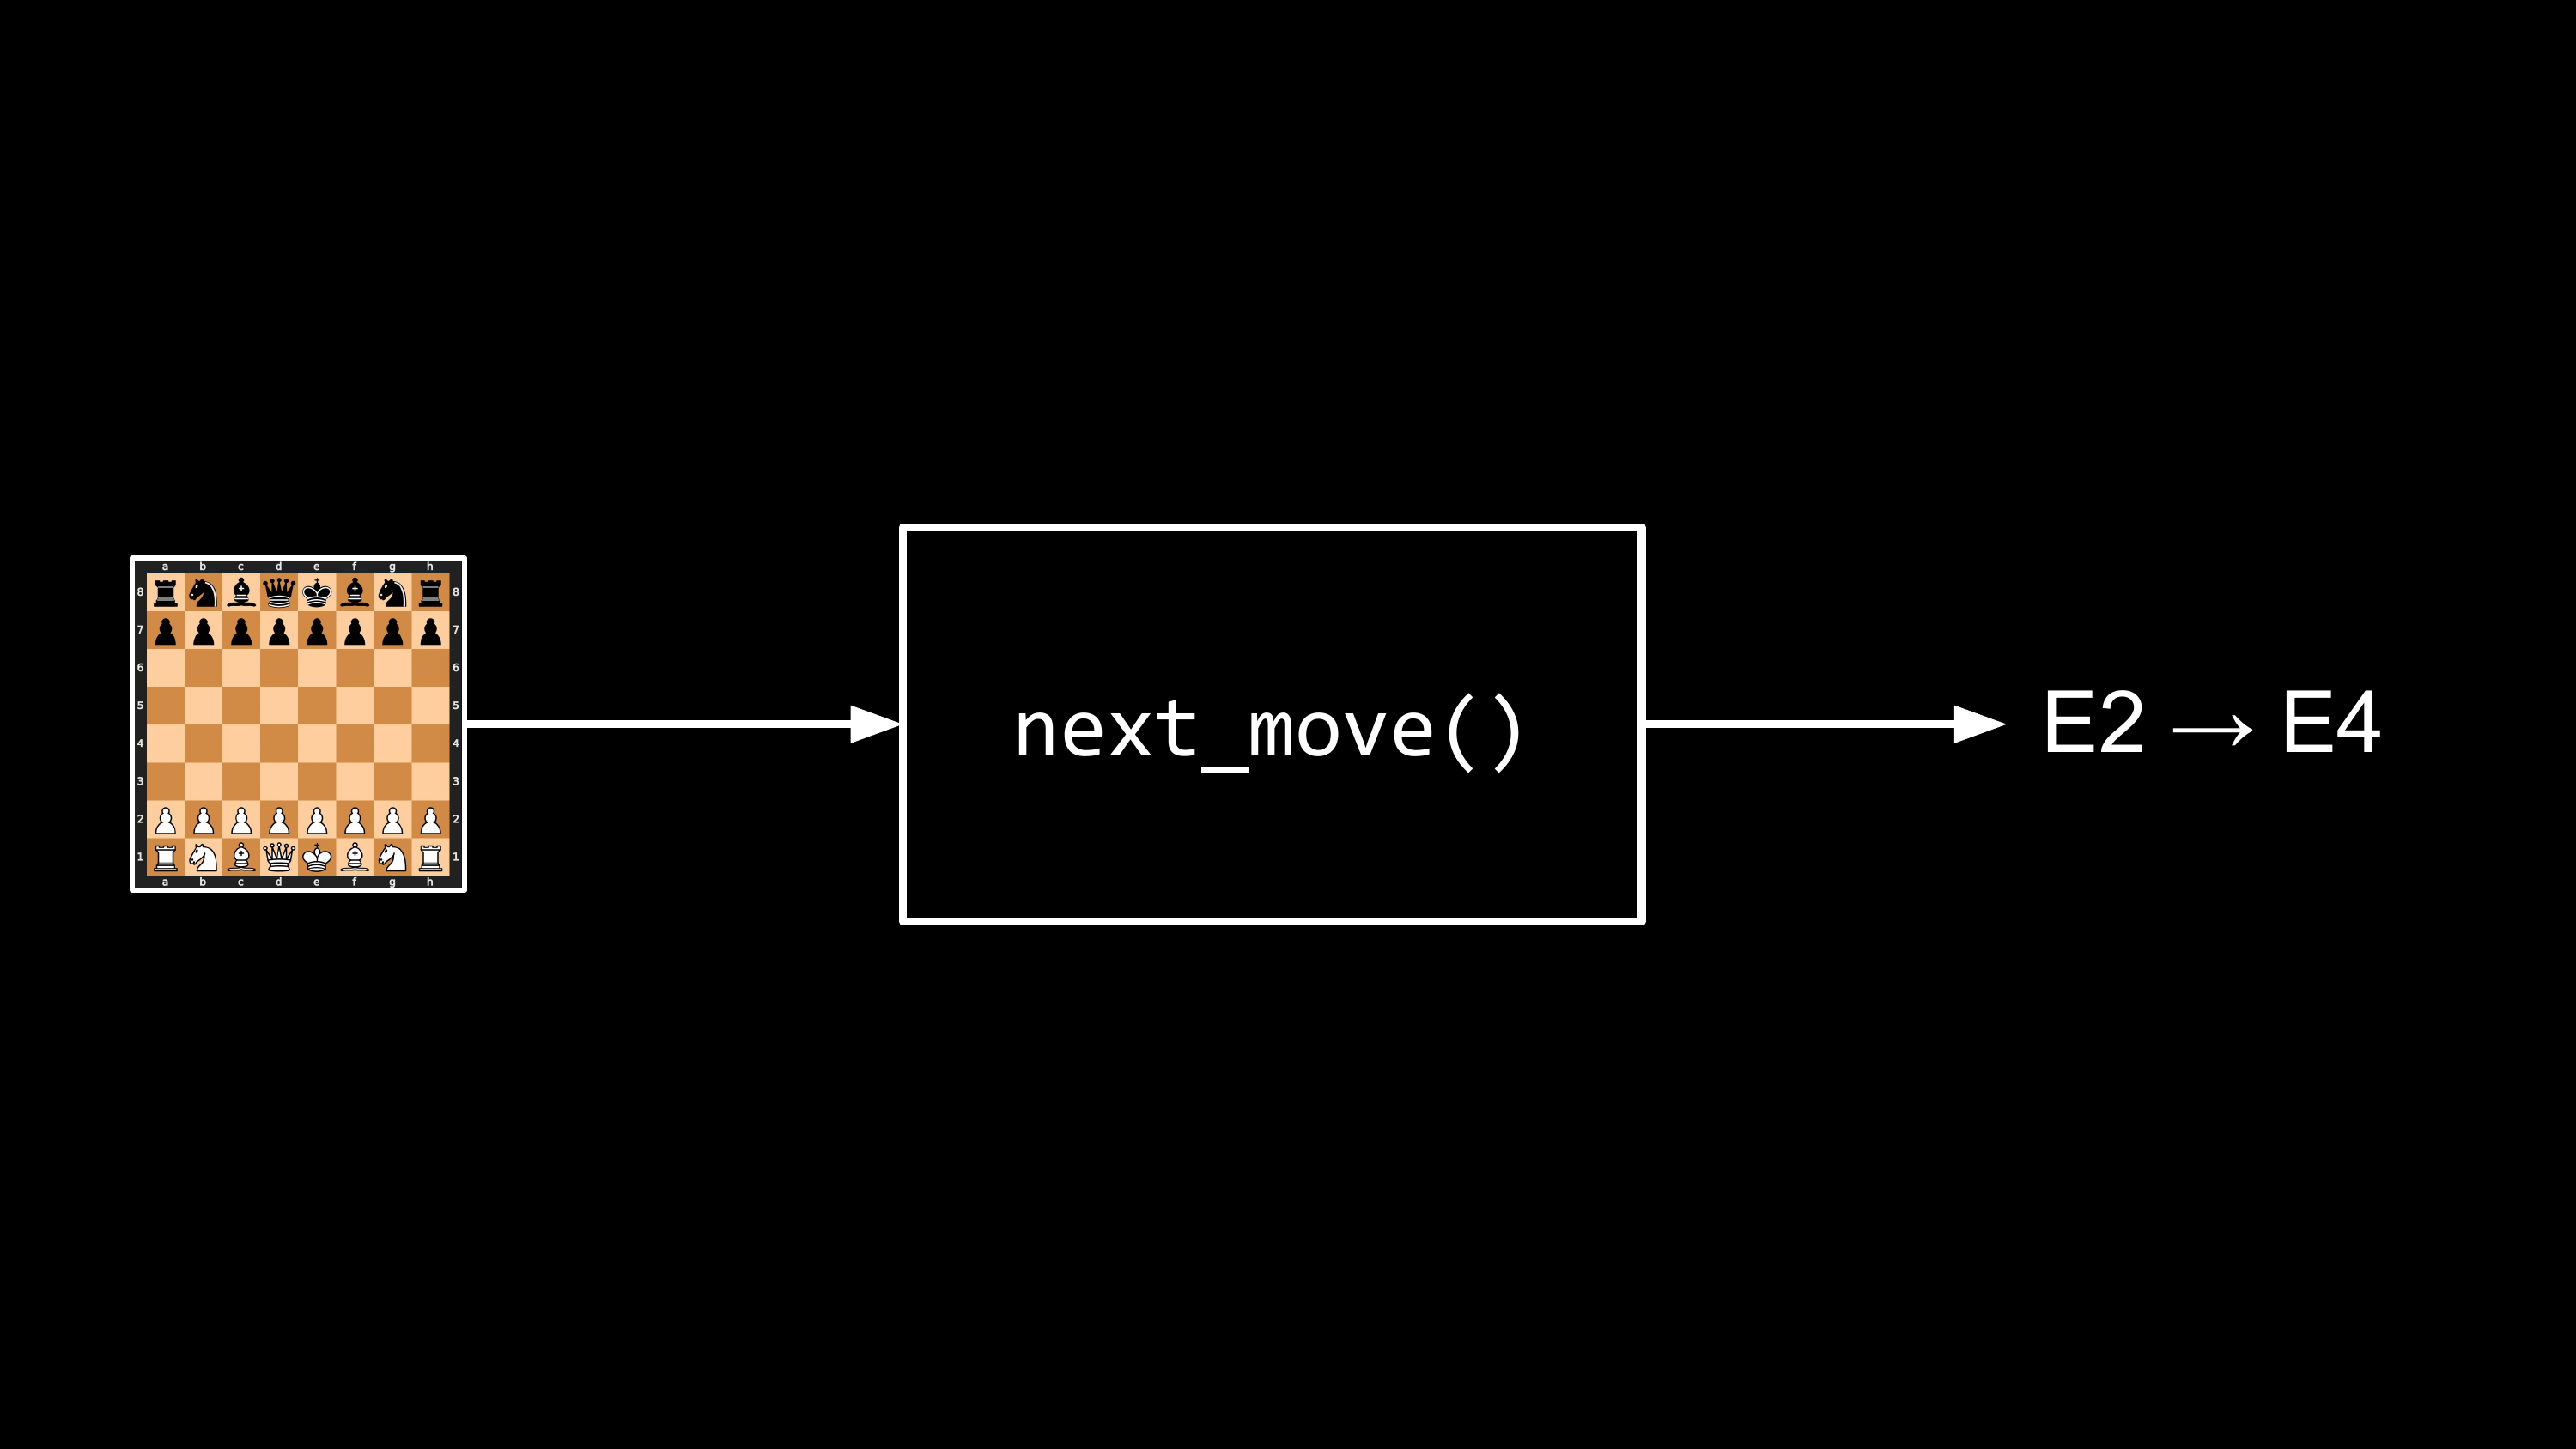
\includegraphics[width=0.6\linewidth,height=\textheight,keepaspectratio]{index_files/mediabag/problem_solving_exam1234.png}
\end{center}

Betrachten wir zunächst die Eingabe für dieses Problem: Wir können dem
Computer nicht einfach ein physisches Schachbrett zeigen, sondern müssen
überlegen, wie sich ein Schachbrett und die Position der Figuren in
digitaler Form darstellen lassen. Dabei kann es durchaus mehrere
Möglichkeiten geben, die uns ans Ziel führen.

Ein Schachbrett lässt sich etwa als Liste von 64 Feldern darstellen, die
von oben links nach unten rechts durchnummeriert sind. Für jedes Feld
speichern wir, ob es leer ist oder welche Figur darauf steht. Die
Figuren werden durch Buchstaben dargestellt -- zum Beispiel ``R'' für
den Turm (Englisch: Rook) oder ``N'' für den Springer (Englisch:
Knight). Für die Farben Schwarz und Weiß verwenden wir einfach 0 und 1.
Diese Darstellungsform reduziert unser Problem auf Listen, Zahlen und
Buchstaben in digitaler Form. Für Computer ist das eine leicht zu
verarbeitende Struktur, wie wir später noch sehen werden. Ein Beispiel
für eine solche Kodierung zeigt
Abbildung~\ref{fig-coding-chess-figures}.

\begin{figure}

\centering{

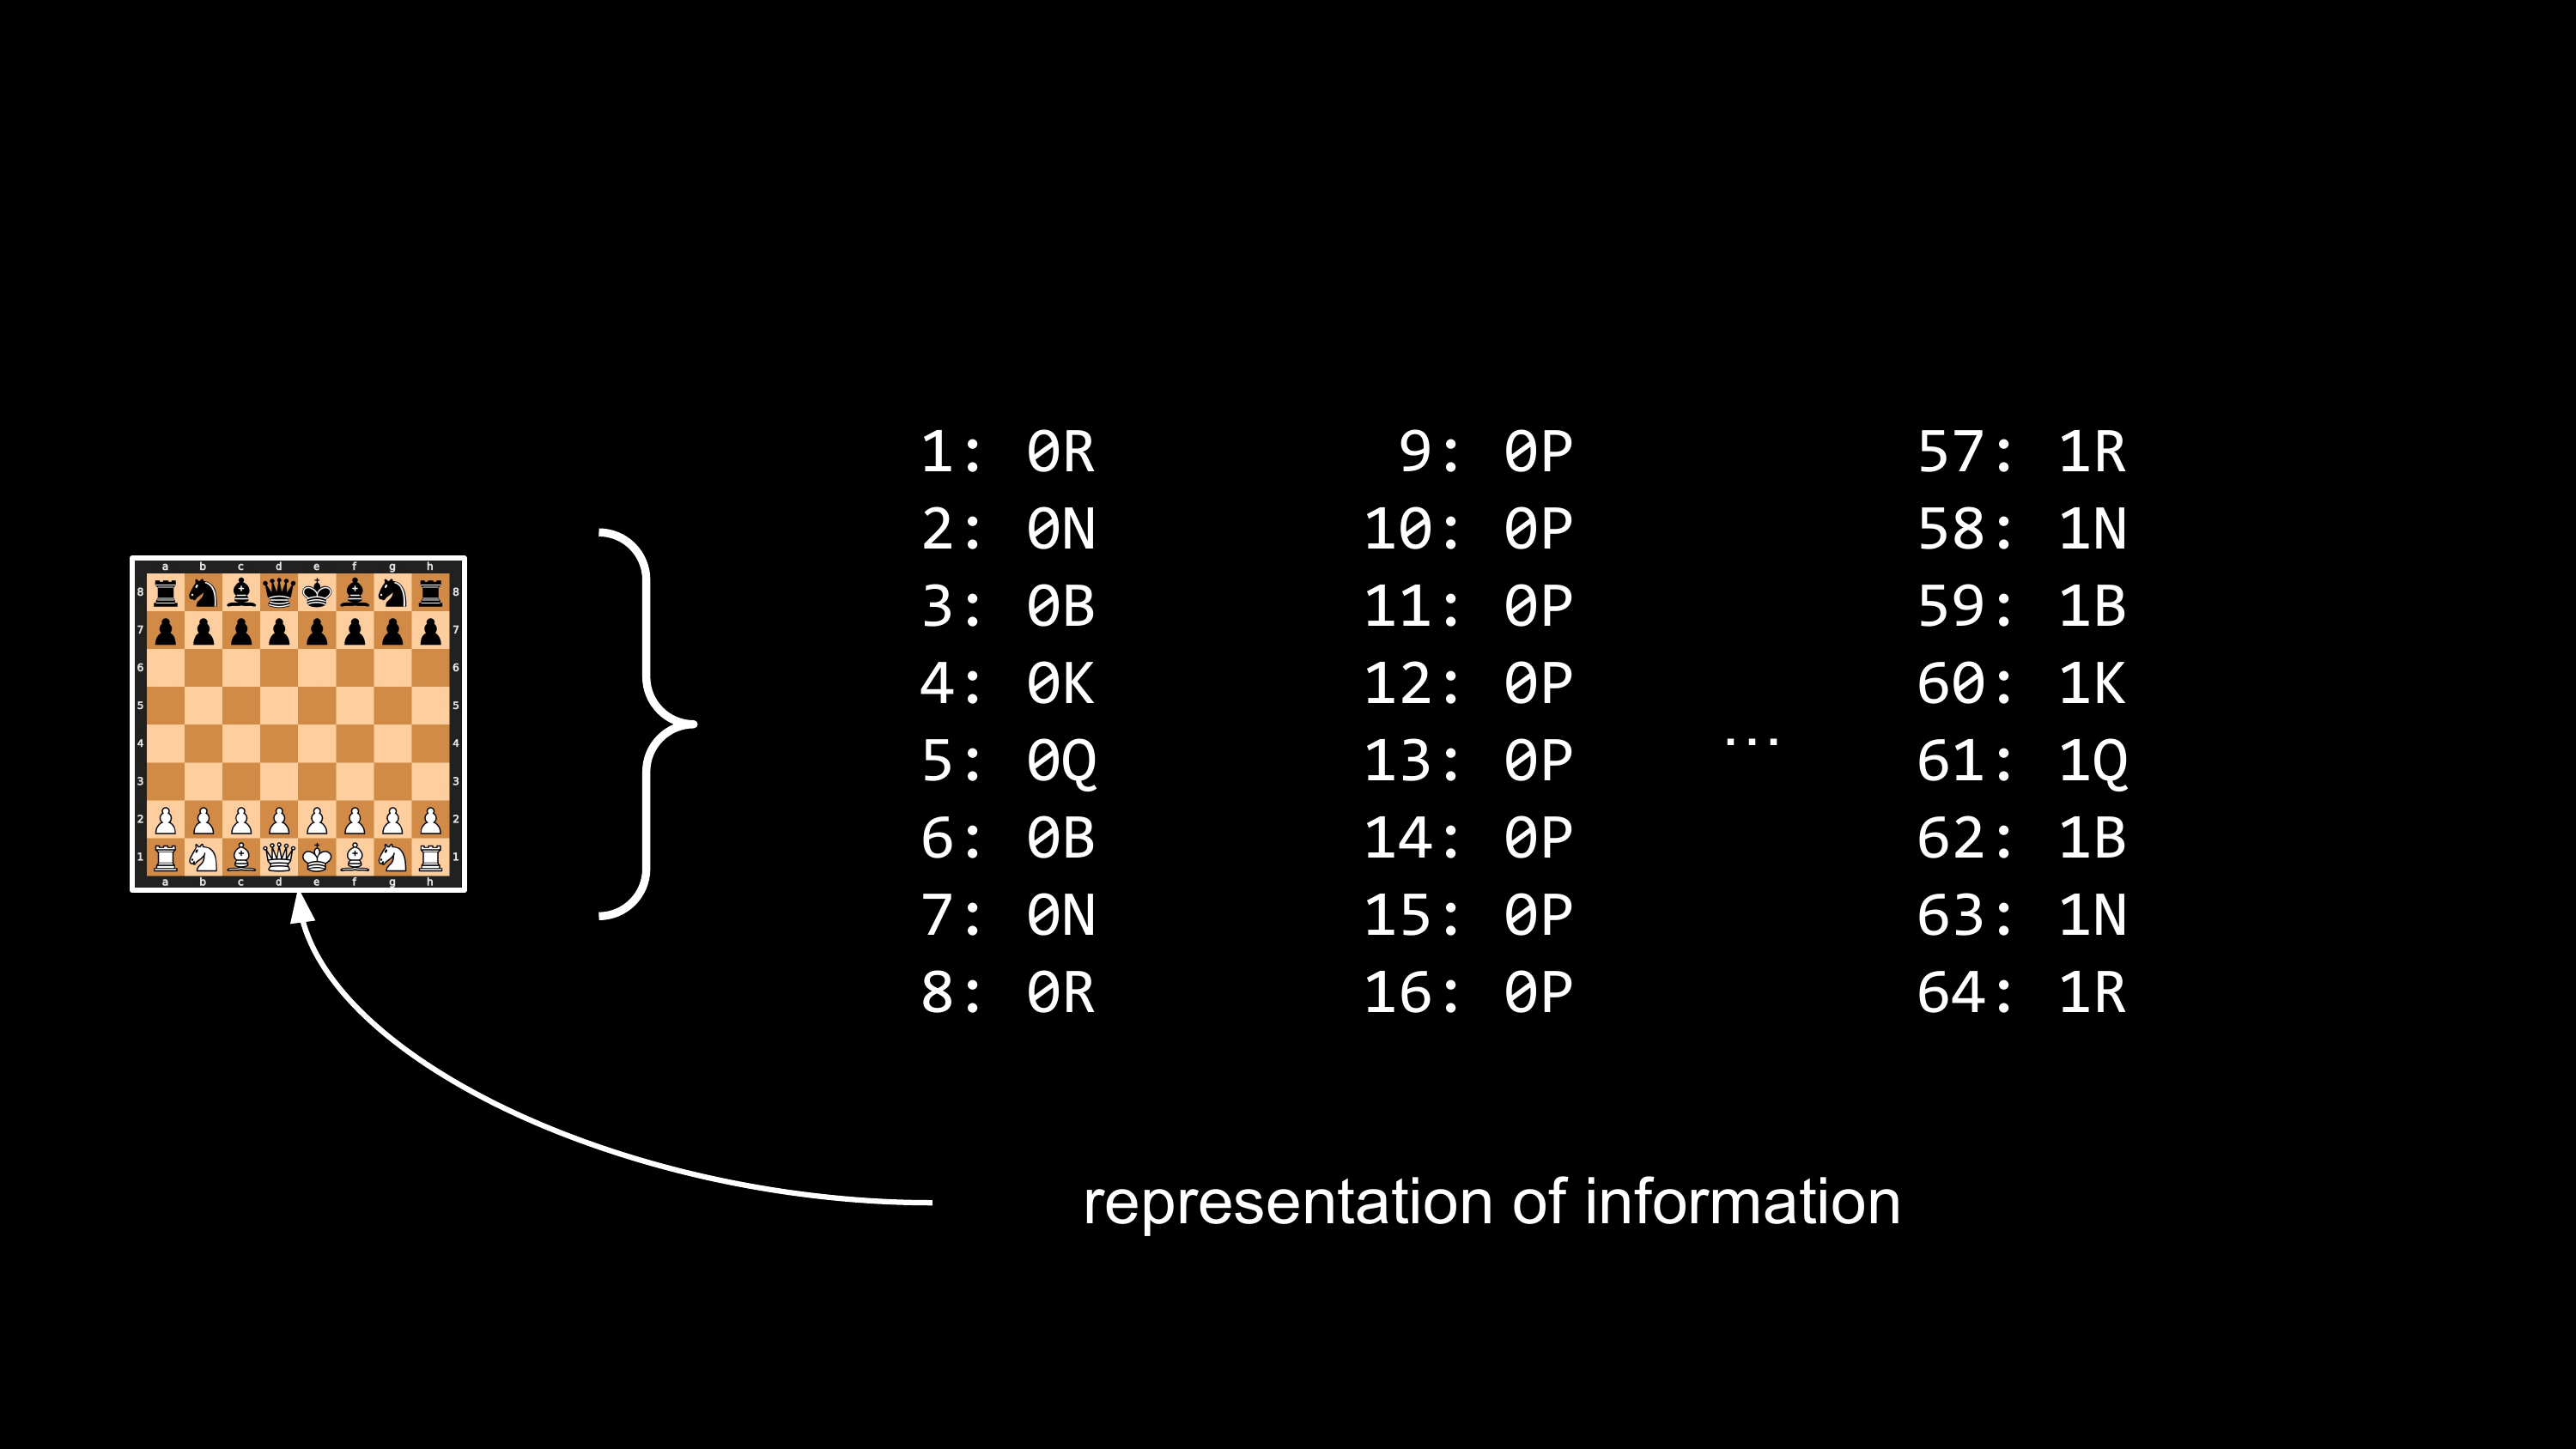
\includegraphics[width=0.6\linewidth,height=\textheight,keepaspectratio]{index_files/mediabag/problem_solving_exam12345.png}

}

\caption{\label{fig-coding-chess-figures}Beispiel für die Darstellung
von Schachfiguren als Zahlen und Buchstaben.}

\end{figure}%

Die Ausgabe, also der nächste Zug, lässt sich ebenfalls durch Zahlen und
Buchstaben darstellen. Eine weit verbreitete Notation gibt zunächst die
Koordinate des Ausgangsfelds an, von dem eine Figur gezogen werden soll,
gefolgt von der Koordinate des Zielfelds. Ein Beispiel wäre der Zug von
``E2 nach E4''. Statt ``E2'' und ``E4'' könnten wir ebenso die
entsprechende Zahl zwischen 1 und 64 aus unserer Liste verwenden, um mit
dem obigen Schema konsistent zu bleiben. Der Zug hieße dann ``53 nach
37''.

\subsubsection{Beispiel: Mit Computern
chatten}\label{beispiel-mit-computern-chatten}

Als drittes Beispiel betrachten wir die Verwendung von Chatprogrammen
wie ChatGPT. Seit seiner Veröffentlichung im November 2022 hat es die
Welt stark verändert und einen regelrechten KI-Hype ausgelöst. Ein
großes Sprachmodell wie GPT-4, das hinter dem heutigen ChatGPT steckt,
ist eine komplexe Software, die wir in diesem Buch nicht vollständig
ergründen können. Das Schöne an Modellen wie dem EVA-Modell ist jedoch,
dass sie komplexe Sachverhalte vereinfachen können -- so auch bei
Sprachmodellen. Das Problem, das Sprachmodelle lösen, lässt sich wie
alle Probleme in unserem EVA-Modell einfach darstellen.

\begin{figure}

\centering{

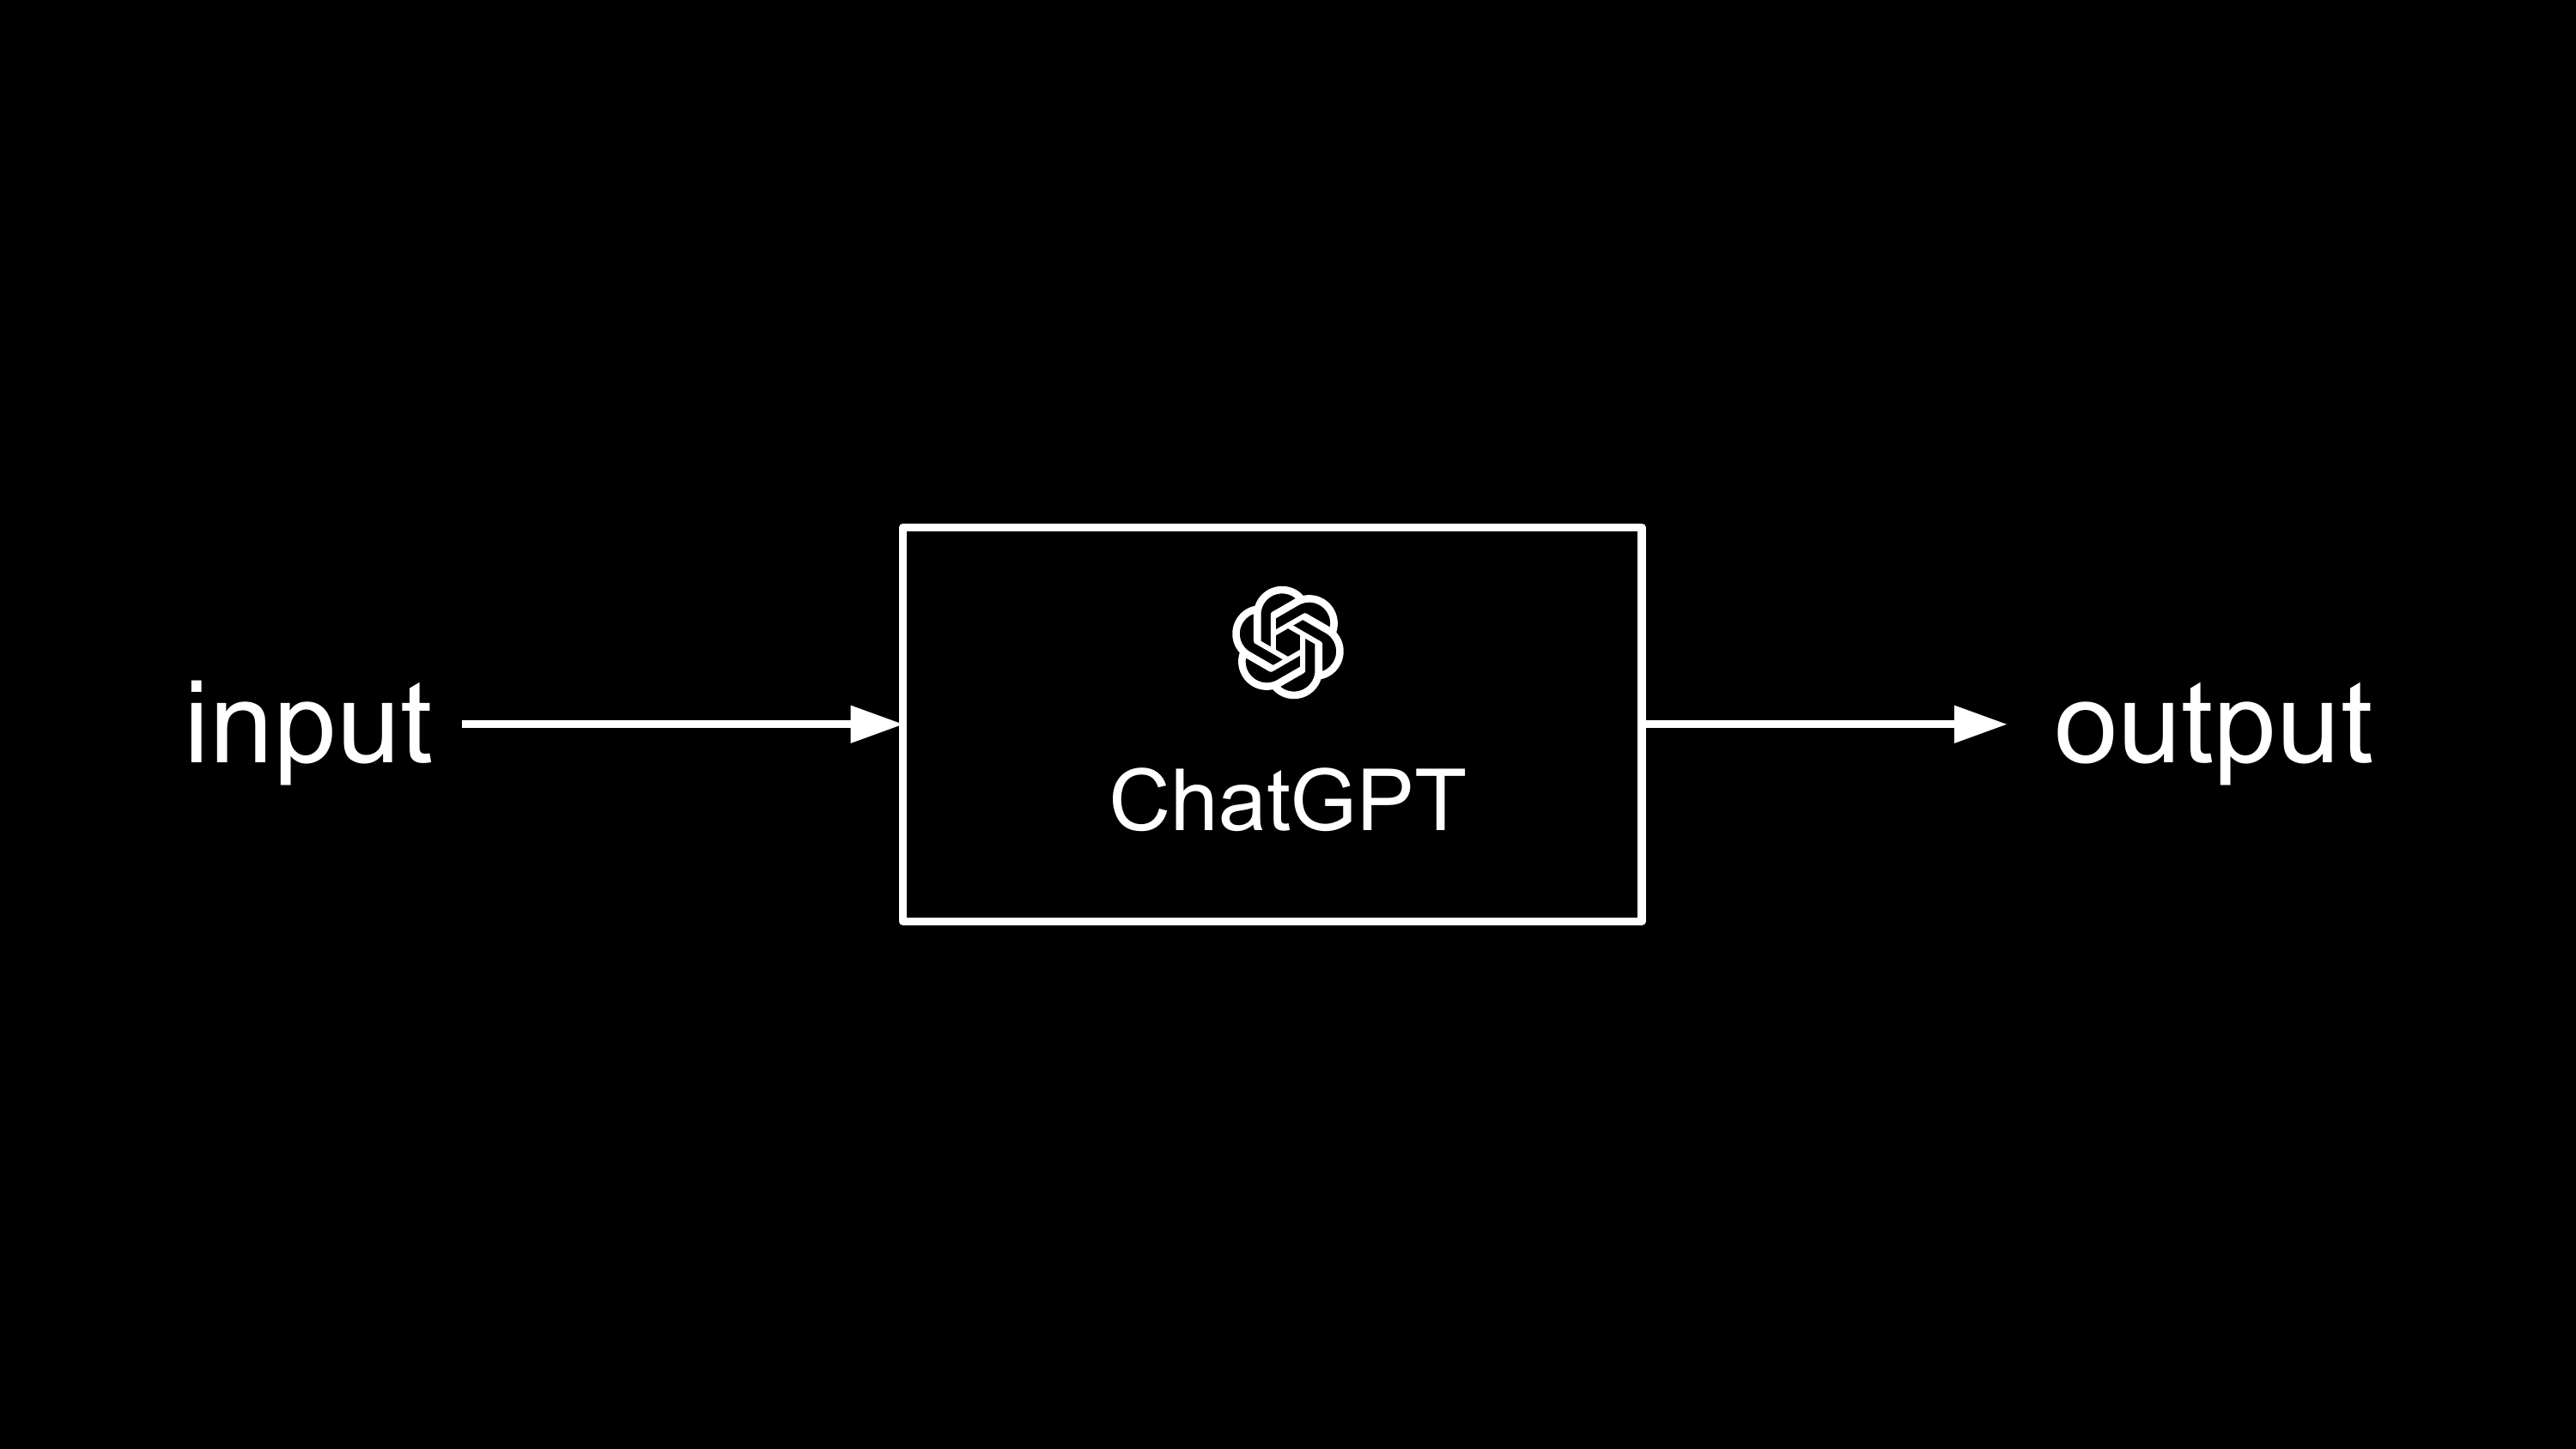
\includegraphics[width=0.6\linewidth,height=\textheight,keepaspectratio]{index_files/mediabag/problem_solving_exam123456.png}

}

\caption{\label{fig-eva-model-example-chatgpt}ChatGPT im EVA-Modell.}

\end{figure}%

Dabei betrachten wir das Sprachmodell -- oder ChatGPT -- als Blackbox,
ohne die internen Prozesse genauer zu definieren. Für unser Modell
genügt es zu verstehen, dass wir eine Eingabe in Form einer Nachricht an
ChatGPT benötigen und als Ausgabe eine Antwort erhalten. Auch hier
stellt sich die Frage, wie wir beides digital repräsentieren können,
damit ChatGPT damit arbeiten kann.

Klassischerweise bestehen sowohl Eingabe als auch Ausgabe einfach aus
Texten -- allerdings beherrschen moderne Sprachmodelle auch andere
Eingabeformen wie Bilder oder gesprochene Sprache über ein Mikrofon. Wir
sprechen dann von multimodalen KI-Modellen. Bei Bildern stehen wir vor
demselben Repräsentationsproblem wie bei unserer Drohnenaufnahme. Bei
der Sprache stellt sich neben der Repräsentation von Audioinhalten die
Frage, wie wir gesprochene Worte überhaupt in eine digitale Form
überführen können. Auch dazu erfahren wir im späteren Verlauf des Buches
mehr.

\subsection{Die Lösung des Problems}\label{die-luxf6sung-des-problems}

Anhand des EVA-Modells wird deutlich, dass wir dem Computer
Informationen in Form von digitalen Daten bereitstellen müssen, mit
denen er arbeiten kann. Was aber genau soll er damit machen? Hier kommt
der mittlere Kasten des Modells ins Spiel -- die eigentliche Lösung des
Problems.

\begin{center}
\includegraphics[width=0.6\linewidth,height=\textheight,keepaspectratio]{index_files/mediabag/problem_solving_inpu123.png}
\end{center}

In der Informatik nennen wir die Beschreibung zur Lösung eines Problems
einen \textbf{Algorithmus}. Ein Algorithmus ist eine
Schritt-für-Schritt-Anleitung zur Problemlösung und ist zunächst
unabhängig von Computern. Das bedeutet, wir können die Lösung eines
Problems ohne Bezug zu einem Computer beschreiben und nennen das einen
Algorithmus.

Stellt euch dazu zum Beispiel eine IKEA-Aufbauanleitung vor. Sie
beschreibt in sequenziellen Schritten, was zu tun ist, um das fertige
Möbelstück zu bekommen. Die Eingabe besteht aus den mitgelieferten
Teilen, Schrauben und dem benötigten Werkzeug für den Zusammenbau. Die
Ausgabe ist das fertige Regal (oder ein anderes Möbelstück) -- und das
alles ganz ohne Computer.

Oder nehmt das Kochrezept eure Lieblingsessens. Auch ein Kochrezept ist
ein Algorithmus: Die Eingabe besteht aus den Zutaten und
Küchenutensilien, die Verarbeitung erfolgt durch die
Schritt-für-Schritt-Anleitung, und die Ausgabe ist das fertige Gericht.
Wie bei der IKEA-Anleitung ist der Algorithmus unabhängig von einem
Computer -- er beschreibt lediglich die Lösung des Problems ``Wie koche
ich dieses Gericht?''.

Zu Beginn des Kapitels haben wir festgestellt, dass Computer aufgrund
ihrer Geschwindigkeit und Fehlerfreiheit besonders gut zur Problemlösung
geeignet sind -- insbesondere bei häufig wiederkehrenden Problemen. Die
beiden genannten Beispiele, das IKEA-Regal und das Kochrezept, eignen
sich allerdings nicht für eine direkte Umsetzung durch Computer. Der
Grund liegt in den analogen Eingaben (Baumaterial, Kochzutaten) und
Ausgaben (Möbelstück, fertige Mahlzeit). Diese kann ein Computer nicht
unmittelbar verarbeiten. Dafür wären Roboter nötig, die mit der
physischen Welt interagieren können. Eine solche Automatisierung lohnt
sich heute nur bei Aufgaben, die sehr häufig auftreten und ansonsten mit
hohen Kosten verbunden sind -- wie etwa in der Automobilindustrie, wo
computergesteuerte Roboter in der Produktion zum Einsatz kommen.

Nehmen wir an, dass Haushaltsroboter in Zukunft erschwinglich werden und
uns beim Kochen unseres Lieblingsgerichts helfen können. Wie vermitteln
wir dann dem Roboter -- im Grunde ein Computer mit Armen und Beinen --
den Algorithmus für unser Rezept? Die Lösung liegt in der
Programmierung: Wir erstellen ein \textbf{Programm} in einer
computerverständlichen Sprache. Dieses Programm wandelt die Anweisungen
aus unserem Kochbuch in Befehle um, die der Computer verstehen und
ausführen kann. Genau genommen besteht ein Programm ebenfalls nur aus
Informationen, und wir müssen herausfinden, wie wir diese Informationen
digital darstellen können. Die Lösung besteht in der Verwendung einer
\textbf{Programmiersprache} wie Python, die wir später kennenlernen
werden.

\section{Welche Strategien gibt es für die Lösung von
Problemen?}\label{welche-strategien-gibt-es-fuxfcr-die-luxf6sung-von-problemen}

Die konkrete Lösung und der zugehörige Algorithmus sehen für jedes
Problem unterschiedlich aus. Das Erkennen von Pflanzen folgt einer
anderen Logik als die Entscheidung, welche Schachfigur als nächstes
gezogen werden soll. Dennoch gibt es universelle Lösungsstrategien, die
auf viele Probleme anwendbar sind, um sie möglichst effizient zu lösen.
Im Folgenden betrachten wir drei dieser Strategien.

\subsection{\texorpdfstring{Problemzerlegung (\emph{Problem
Decomposition})}{Problemzerlegung (Problem Decomposition)}}\label{problemzerlegung-problem-decomposition}

Eine universelle Strategie zur Lösung komplexer Probleme ist die
Zerlegung in kleinere Schritte oder Teilprobleme. Jedes dieser
Teilprobleme ist unterschiedlich und erfordert einen spezifischen
Lösungsansatz. Nehmen wir als Beispiel das Zählen von Pflanzen auf einer
Drohnenaufnahme. Dieses komplexe Problem lässt sich, ausgehend von der
Eingabe -- dem digitalen Bild -- in drei Teilprobleme zerlegen:

\begin{enumerate}
\def\labelenumi{\arabic{enumi}.}
\item
  Pflanzen auf dem Bild lokalisieren
\item
  Lokalisierte Pflanzen klassifizieren: Maispflanze oder nicht?
\item
  Identifizierte Maispflanzen zählen
\end{enumerate}

\begin{center}
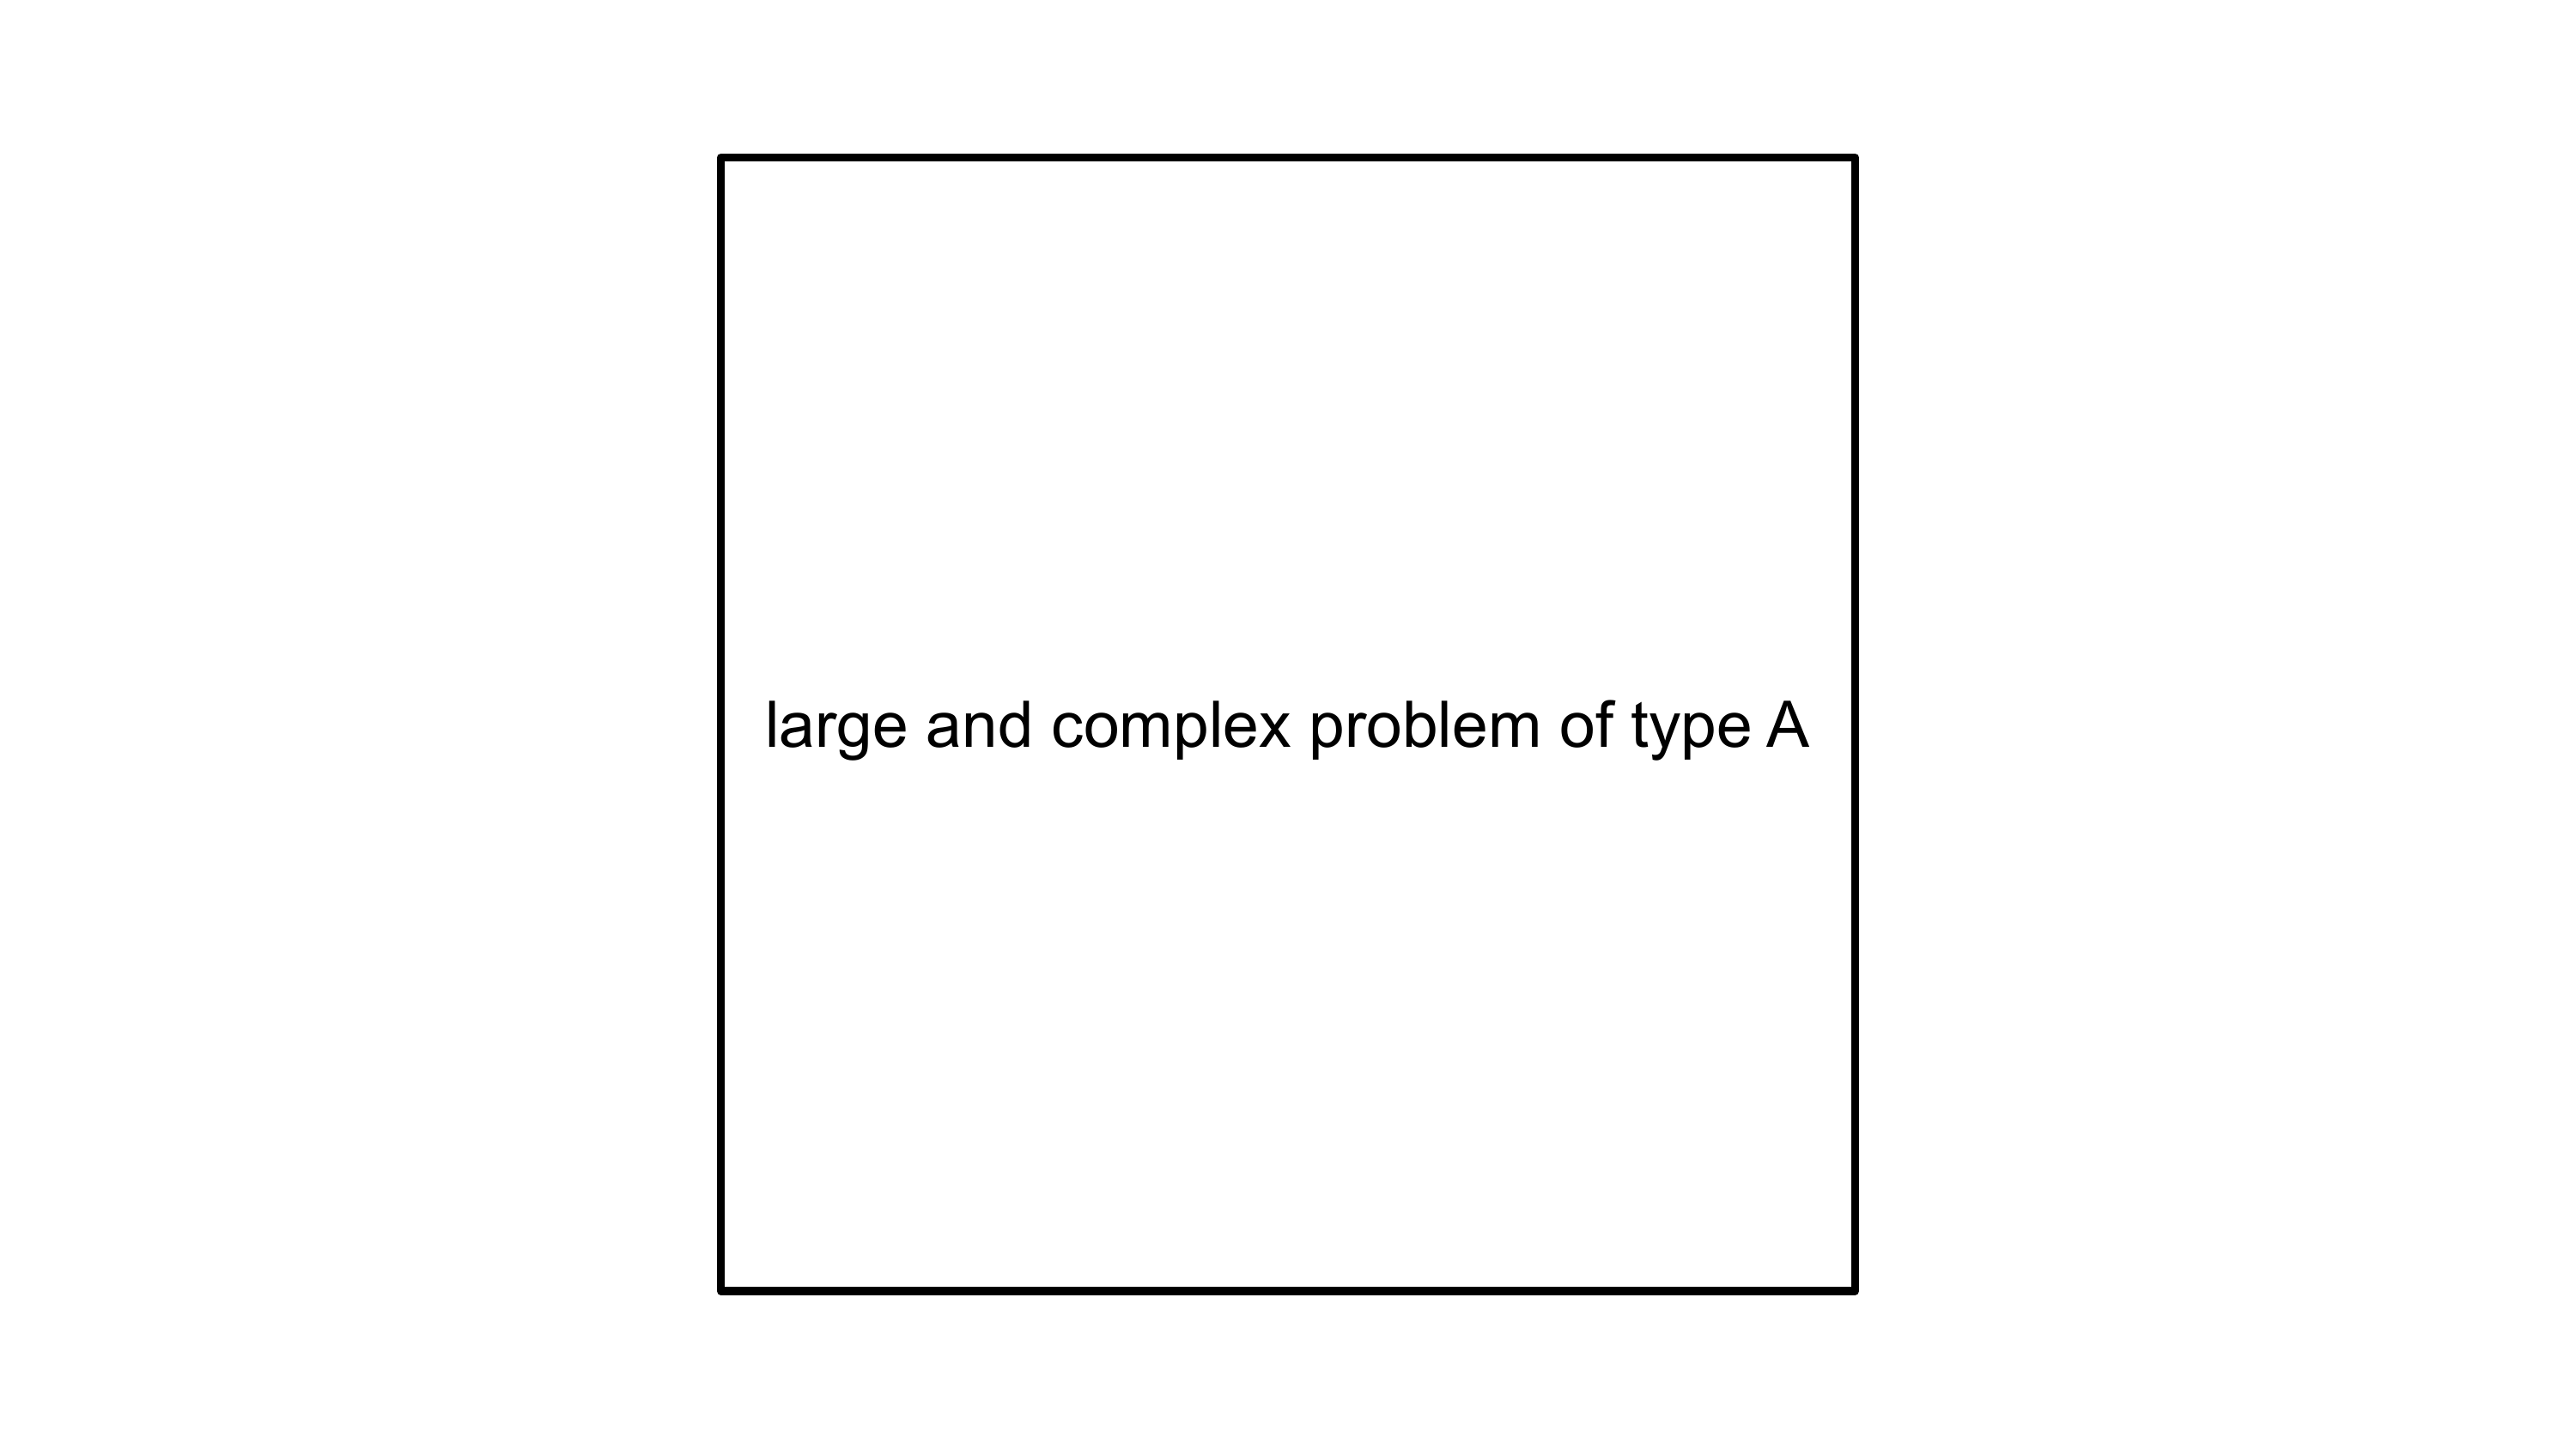
\includegraphics[width=0.6\linewidth,height=\textheight,keepaspectratio]{index_files/mediabag/problem_solving_larg.png}
\end{center}

Jedes dieser Teilprobleme erfordert einen eigenen Algorithmus. Dabei ist
es möglich, die Teilprobleme noch weiter zu zerlegen, um sie besser
bearbeiten zu können.

\begin{center}
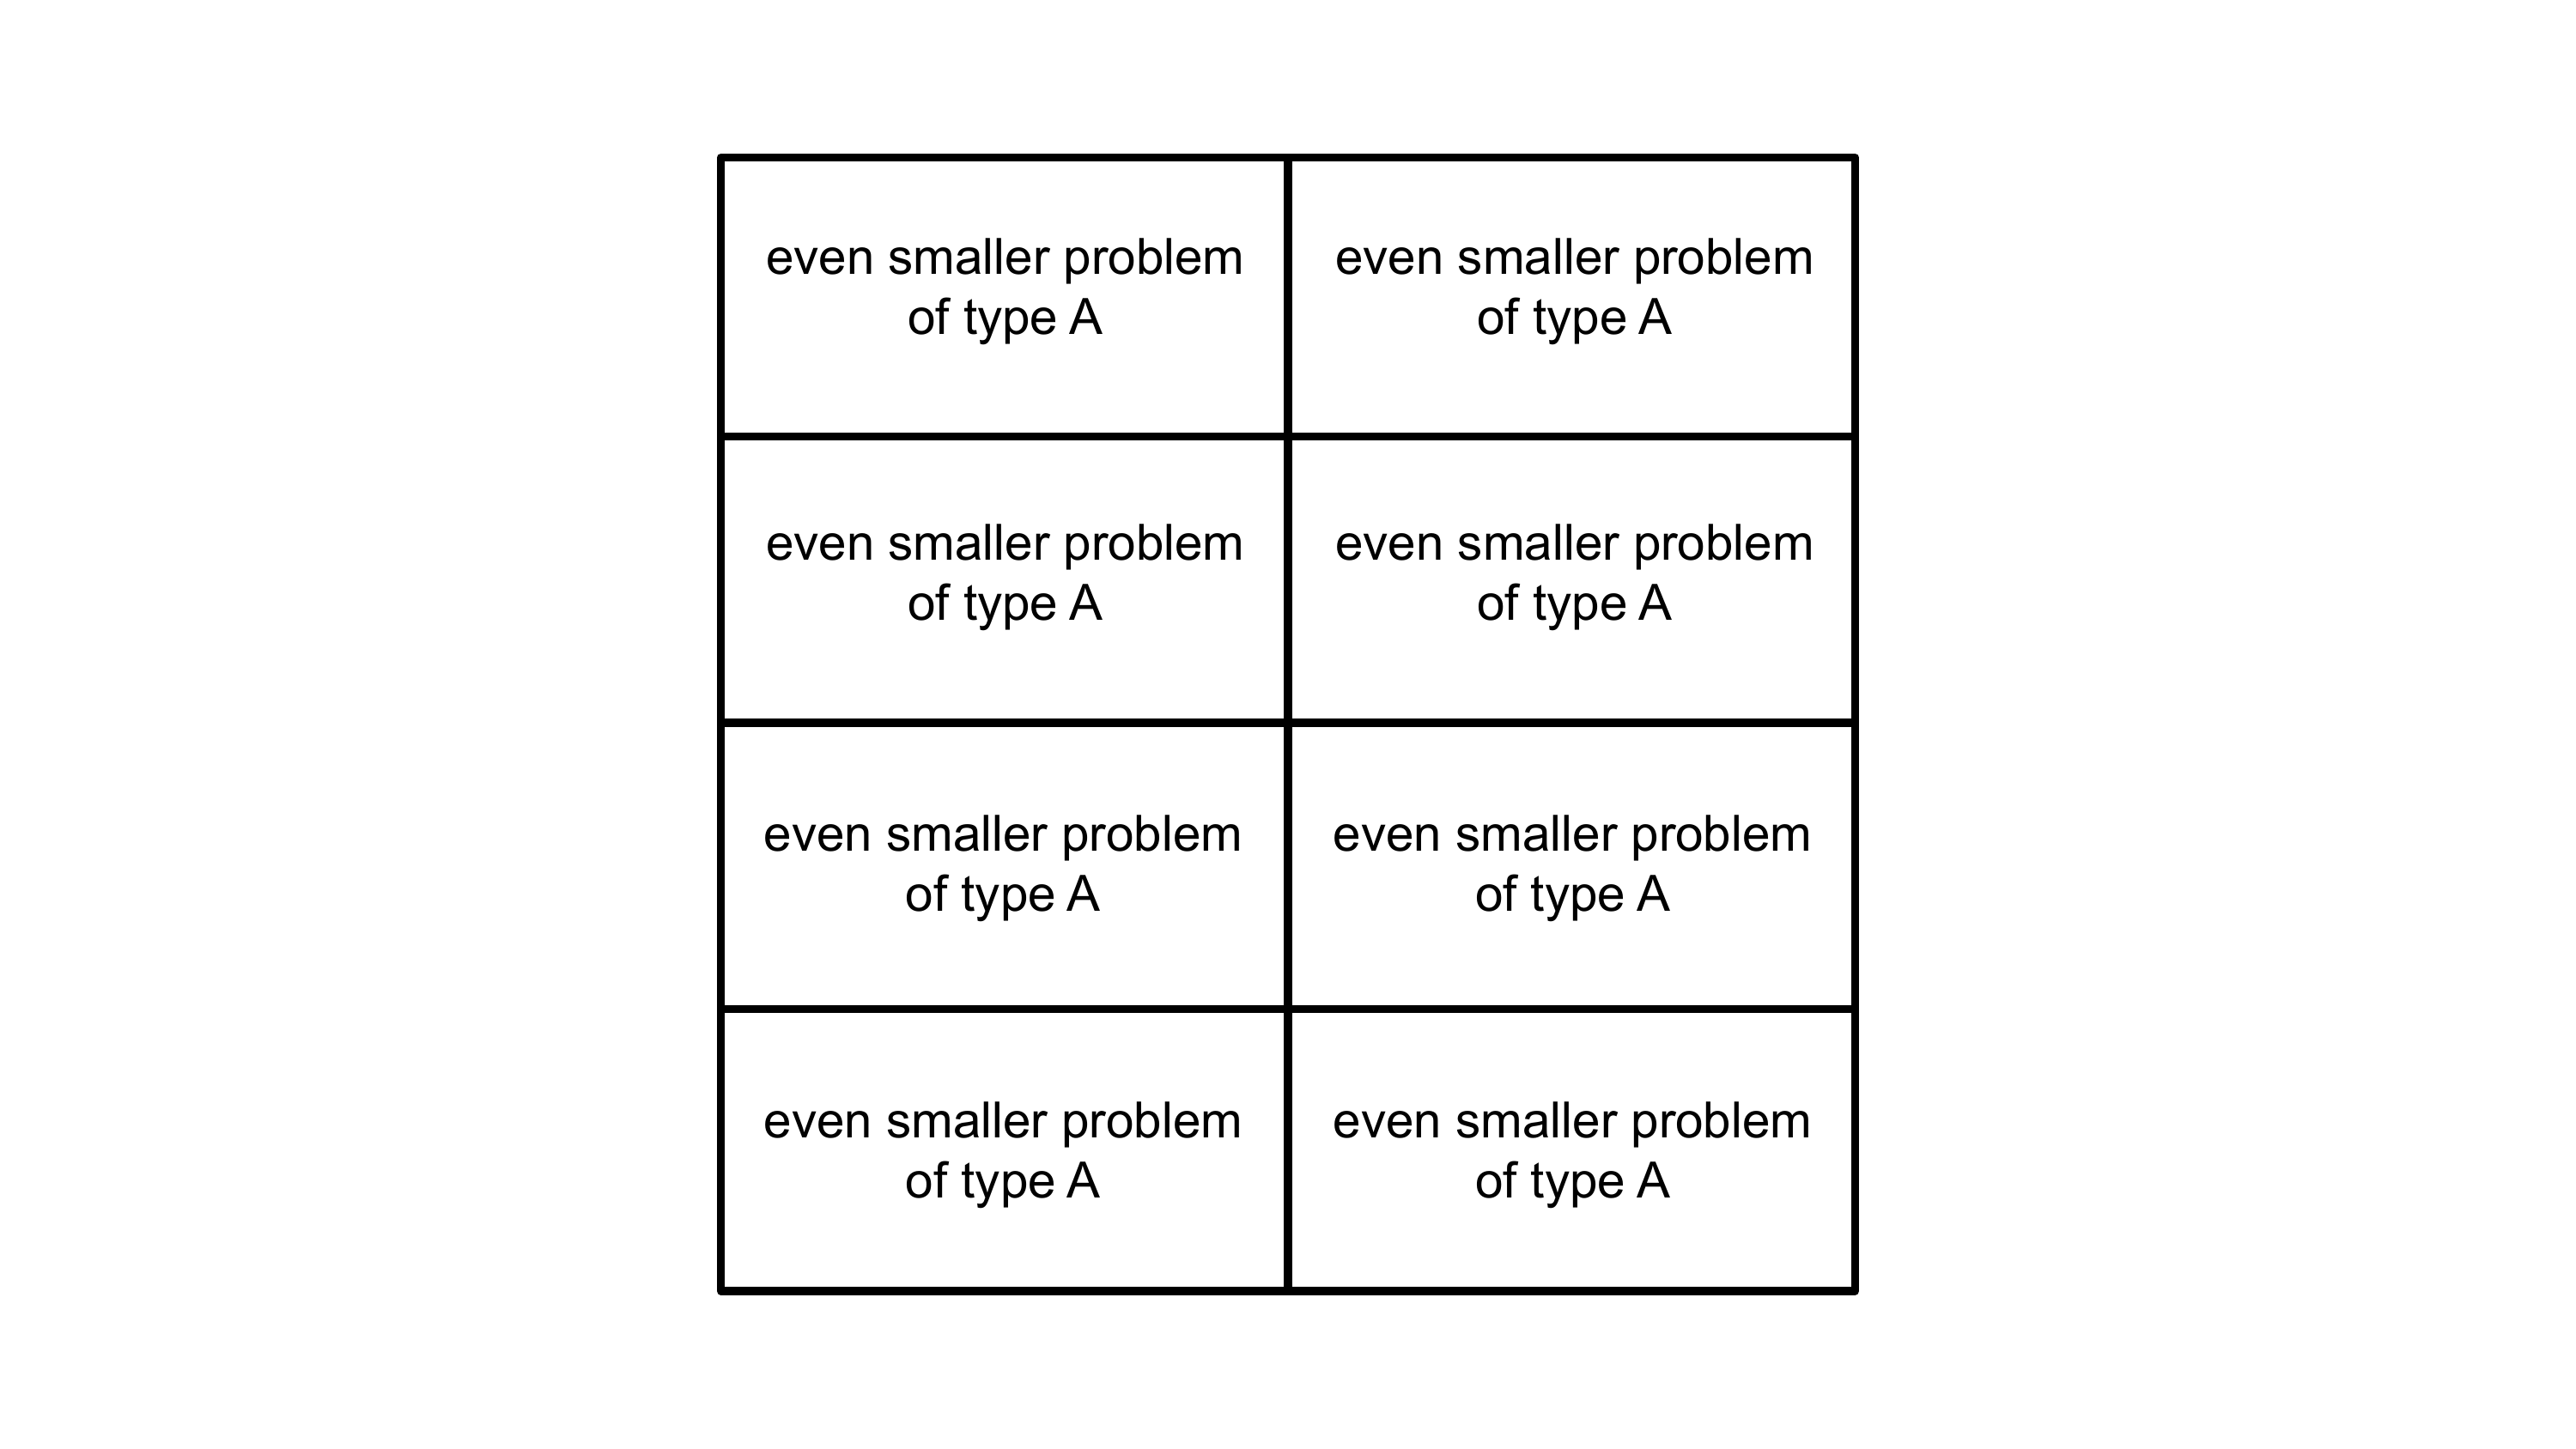
\includegraphics[width=0.6\linewidth,height=\textheight,keepaspectratio]{index_files/mediabag/problem_solving_even.png}
\end{center}

Die Identifizierung sinnvoller Teilprobleme erfordert ein ausgeprägtes
analytisches Denkvermögen. Dies ist besonders wichtig im Umgang mit
Computern. Wie wir beim Erlernen der Programmierung sehen werden, ist
die Zerlegung eines Problems in kleine, lösbare Schritte der Schlüssel
zur Beherrschung seiner Komplexität.

\subsection{\texorpdfstring{Teile und Herrsche (\emph{Divide and
Conquer})}{Teile und Herrsche (Divide and Conquer)}}\label{teile-und-herrsche-divide-and-conquer}

Die ``Teile und Herrsche''-Strategie ist ein Ansatz zur Lösung komplexer
Probleme, bei dem wir das Hauptproblem schrittweise in immer kleinere
Teilprobleme zerlegen, bis diese einfach zu lösen sind. Dabei gehen wir
rekursiv vor: Wir teilen das ursprüngliche Problem in kleinere Teile,
diese kleineren Probleme wiederum in noch kleinere Teile und so weiter.
Die Rekursion endet, wenn die Probleme so klein sind, dass sie sich
nicht weiter aufteilen lassen und die Lösung direkt ersichtlich ist.

Anders als bei der Problemzerlegung sind die Teilprobleme beim Divide
and Conquer-Ansatz dadurch gleichartig und stellen nur kleinere
Instanzen des ursprünglichen Problems dar. Die einzelnen Lösungen für
jedes Teilproblem werden dann schrittweise wieder zusammengeführt, um
die Gesamtlösung zu erhalten. Ein klassisches Beispiel ist die
Sortierung einer langen Liste von Zahlen: Wir teilen die Liste immer
wieder in der Mitte, bis nur noch einzelne Zahlen übrig sind, und fügen
diese dann in sortierter Reihenfolge wieder zusammen.

Ein anderes Beispiel ist die binäre Suche in einer sortierten Liste.
Hier betrachten wir das Element in der Mitte der Liste und vergleichen
es mit dem gesuchten Element. Da die Liste sortiert ist, können wir
entscheiden, in welchem Teil der Liste wir weitersuchen müssen. Im
zweiten Schritt suchen wir nur in diesem Teil weiter und haben damit das
Problem halbiert. Die Natur des Problems bleibt dabei gleich, und wir
können erneut genauso verfahren -- so lange, bis wir nur noch ein
Element übrig haben, das entweder das gesuchte Element ist oder nicht.

\begin{center}
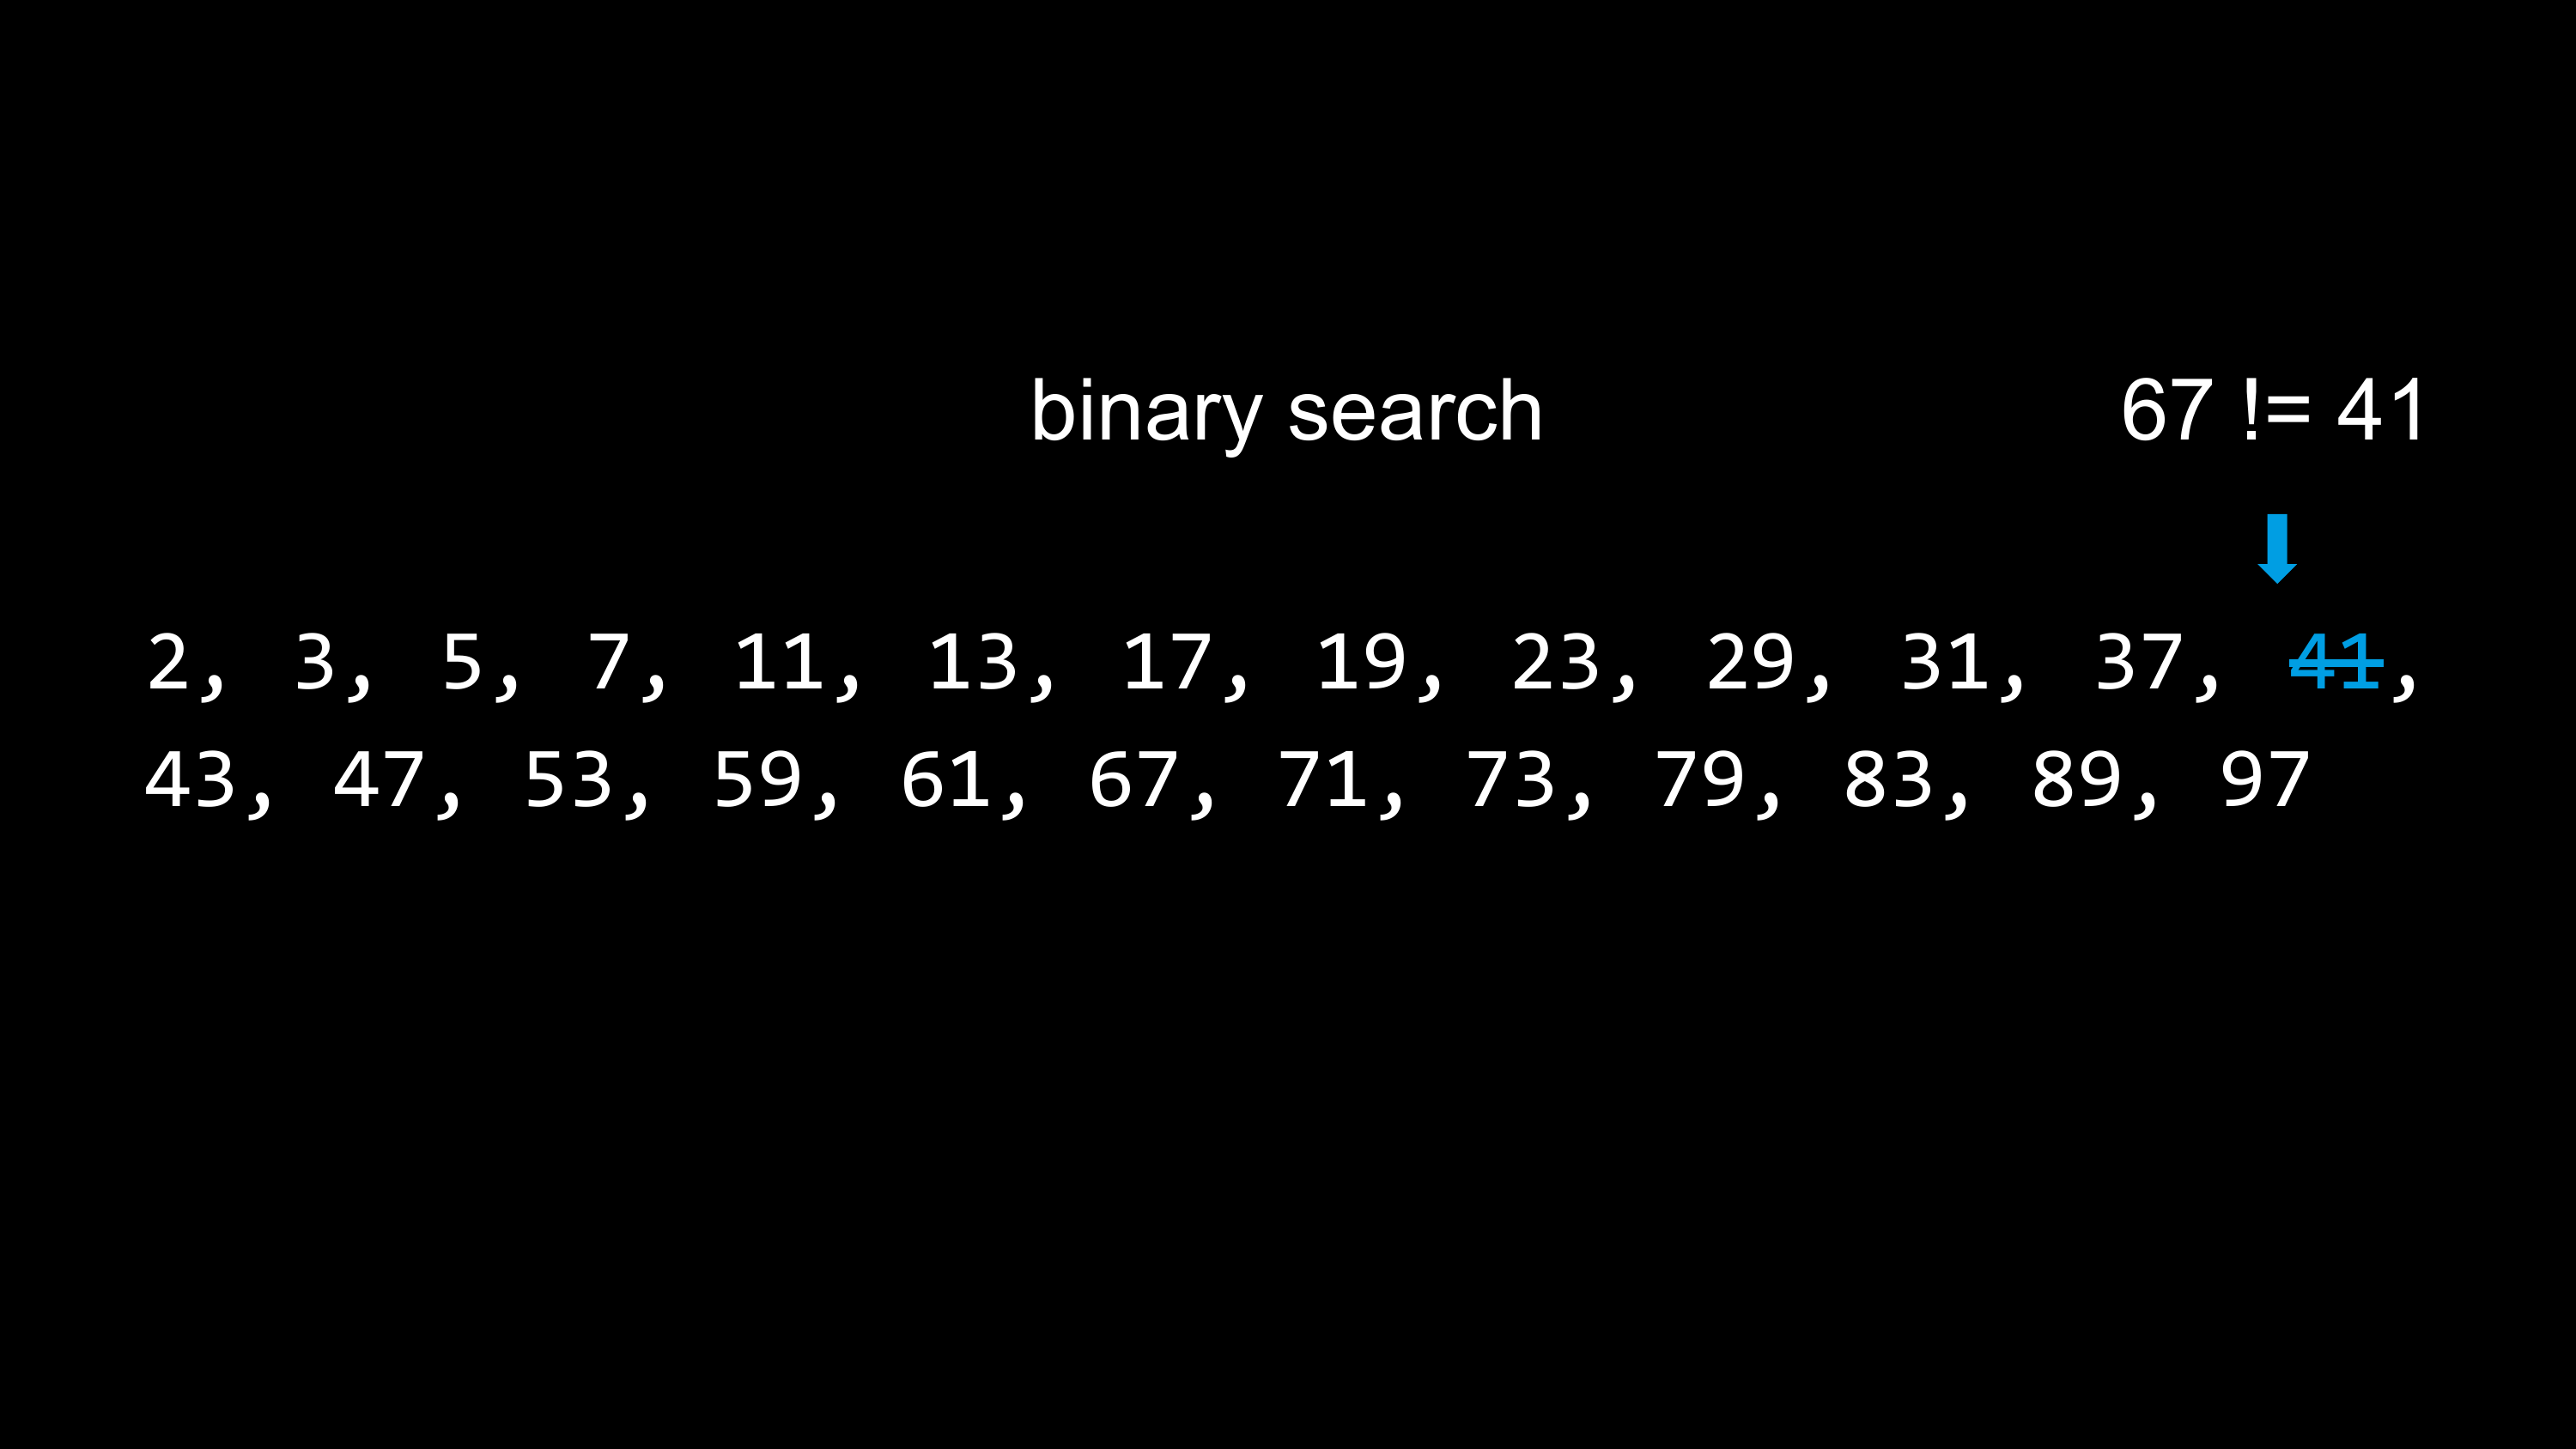
\includegraphics[width=0.6\linewidth,height=\textheight,keepaspectratio]{index_files/mediabag/problem_solving_67_p.png}
\end{center}

\subsection{\texorpdfstring{Verteile und Parallelisiere
(\emph{Distribute and
Parallelize})}{Verteile und Parallelisiere (Distribute and Parallelize)}}\label{verteile-und-parallelisiere-distribute-and-parallelize}

Manche Probleme lassen sich effizienter lösen, wenn mehrere Personen
gleichzeitig daran arbeiten. Anstatt eine einzelne Person mit der
gesamten Aufgabe zu betrauen, verteilen wir die Arbeit auf mehrere
Schultern und arbeiten parallel an der Lösung. Allerdings eignet sich
nicht jedes Problem für diesen Ansatz.

Ein gutes Beispiel ist das Aufräumen eines Zimmers: Eine einzelne Person
müsste nacheinander verschiedene Bereiche aufräumen, während mehrere
Personen gleichzeitig unterschiedliche Ecken des Raums in Angriff nehmen
können. Je größer das Zimmer, desto mehr Personen werden benötigt, um es
in der gleichen Zeit aufzuräumen. Ein Gegenbeispiel, bei dem diese
Strategie nicht funktioniert, ist das Lösen einer mathematischen
Gleichung. Hier müssen die einzelnen Rechenschritte aufeinander
aufbauen, weshalb das Problem nicht gleichzeitig an mehrere Personen
übergeben werden kann, die unabhängig daran arbeiten.

Die Strategie des Verteilens und Parallelisierens -- im Englischen
\emph{Distribute and Parallelize} -- funktioniert nach einem klaren
Prinzip: Wir zerlegen ein großes Problem in Teile, die unabhängig
voneinander gelöst werden können. Diese Teile weisen wir dann
verschiedenen Ressourcen zu -- zum Beispiel mehreren Personen oder
Computern. Jede Ressource arbeitet an ihrem Teilproblem und erzeugt ein
eigenes Ergebnis. Dabei gehen wir davon aus, dass sich alle
Teilergebnisse am Ende zu einer Gesamtlösung zusammenfügen lassen.
Ähnlich wie beim Divide and Conquer-Ansatz sind die Teilprobleme meist
gleichartig.

Um dieses Konzept greifbar zu machen, schauen wir uns ein konkretes
Beispiel an, das wir mit dem EVA-Modell analysieren: das Zählen aller
Wörter in einem Buch.

\begin{figure}[H]

{\centering 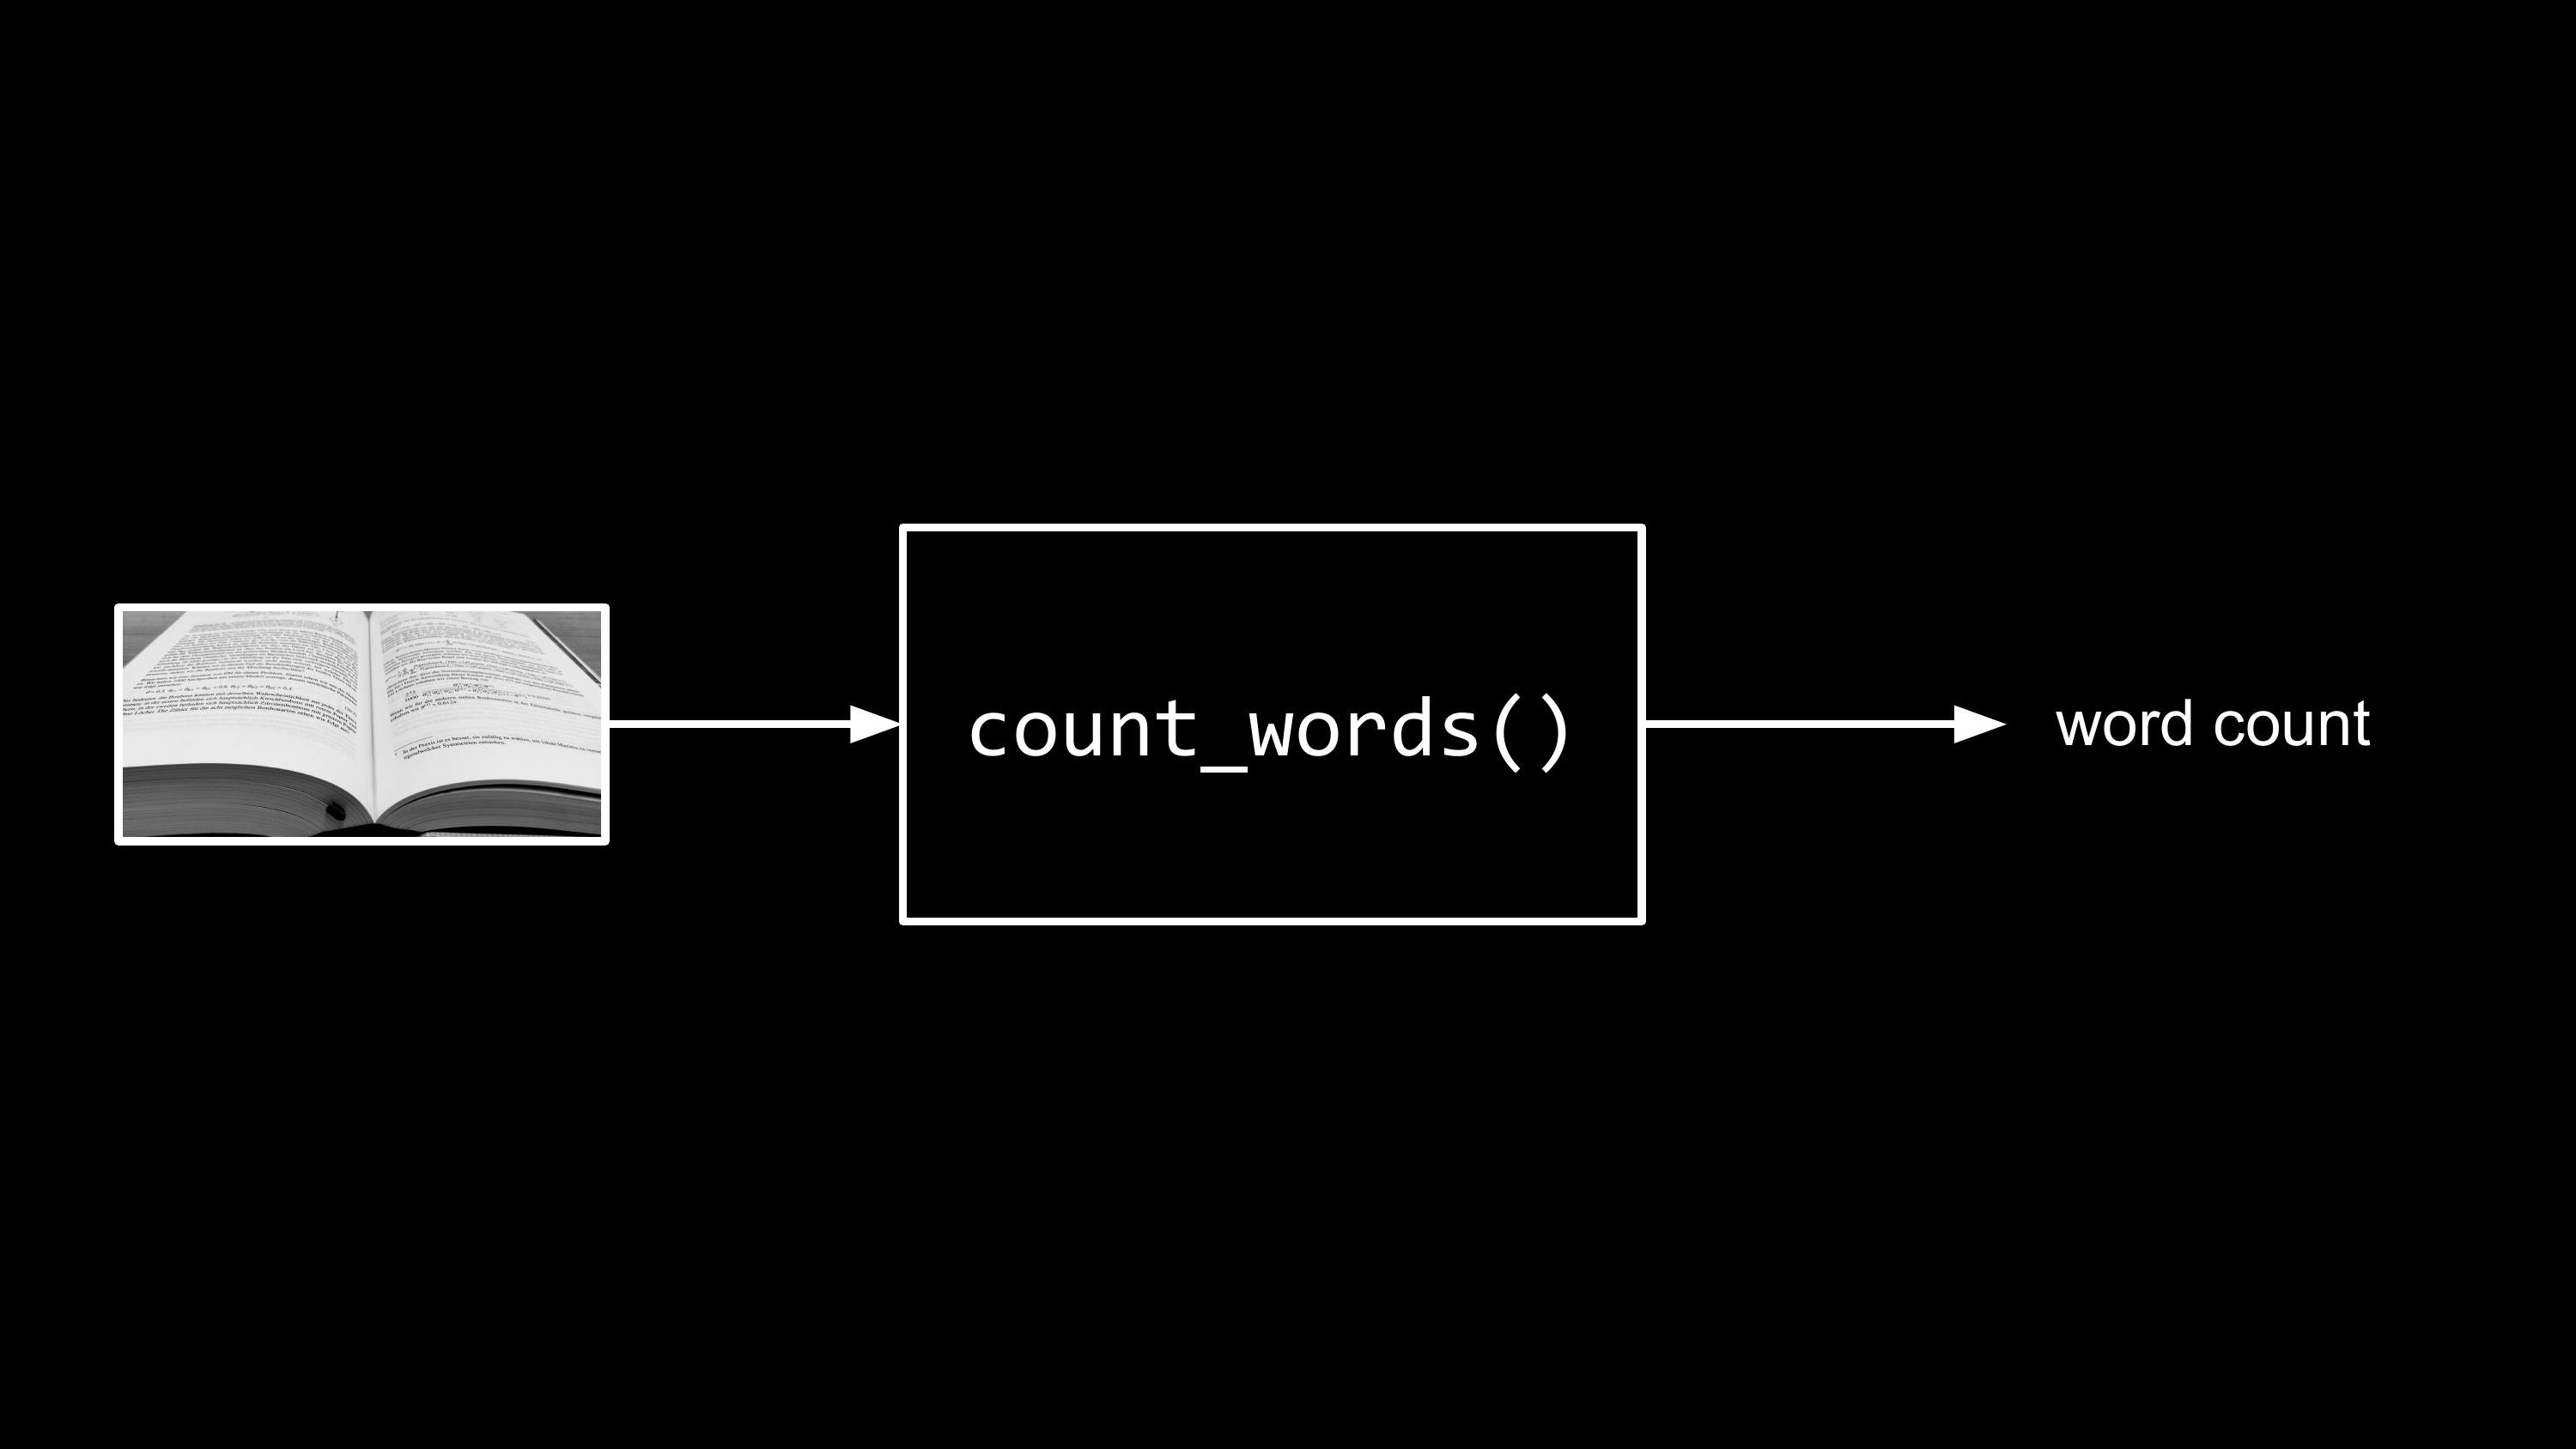
\includegraphics[width=0.6\linewidth,height=\textheight,keepaspectratio]{index_files/mediabag/problem_solving_exam1234567.png}

}

\caption{Das Wörterzählen-Problem im EVA-Modell}

\end{figure}%

Je nach Umfang des Buches kann dies eine mühsame Aufgabe sein, besonders
für Menschen. Ein Computer bewältigt ein einzelnes Buch dank seiner
hohen Verarbeitungsgeschwindigkeit problemlos. Allerdings lässt sich das
Problem beliebig erweitern -- etwa wenn wir statt eines Buches alle
Texte im Internet oder sämtliche Wikipedia-Artikel analysieren möchten.
In solchen Fällen wird die Aufgabe auch für Computer aufwendig und
zeitintensiv. Eine Lösung besteht darin, mehrere Computer parallel
einzusetzen.

In Abbildung~\ref{fig-problem-solving-word-count-distributed} sehen wir
beispielhaft die Verteilung der Buchseiten auf vier Studenten. Jeder
erhält einen gleichen Anteil, wodurch sich die Bearbeitungszeit im
Optimalfall auf ein Viertel reduziert. Bei Computern können wir analog
vorgehen und mehrere Rechner gleichzeitig mit Teilen der Seiten
betrauen. Diese Rechner werden in einem Netzwerk verbunden und von einem
zentralen Computer gesteuert, der die Teilergebnisse am Ende
zusammenführt. Ein solches System nennen wir Rechencluster, bestehend
aus Arbeitern -- den \emph{Worker Nodes} -- sowie einer Steuereinheit,
die in solchen Systemen als \emph{Driver} oder \emph{Name Node}
bezeichnet wird.

\begin{figure}

\centering{

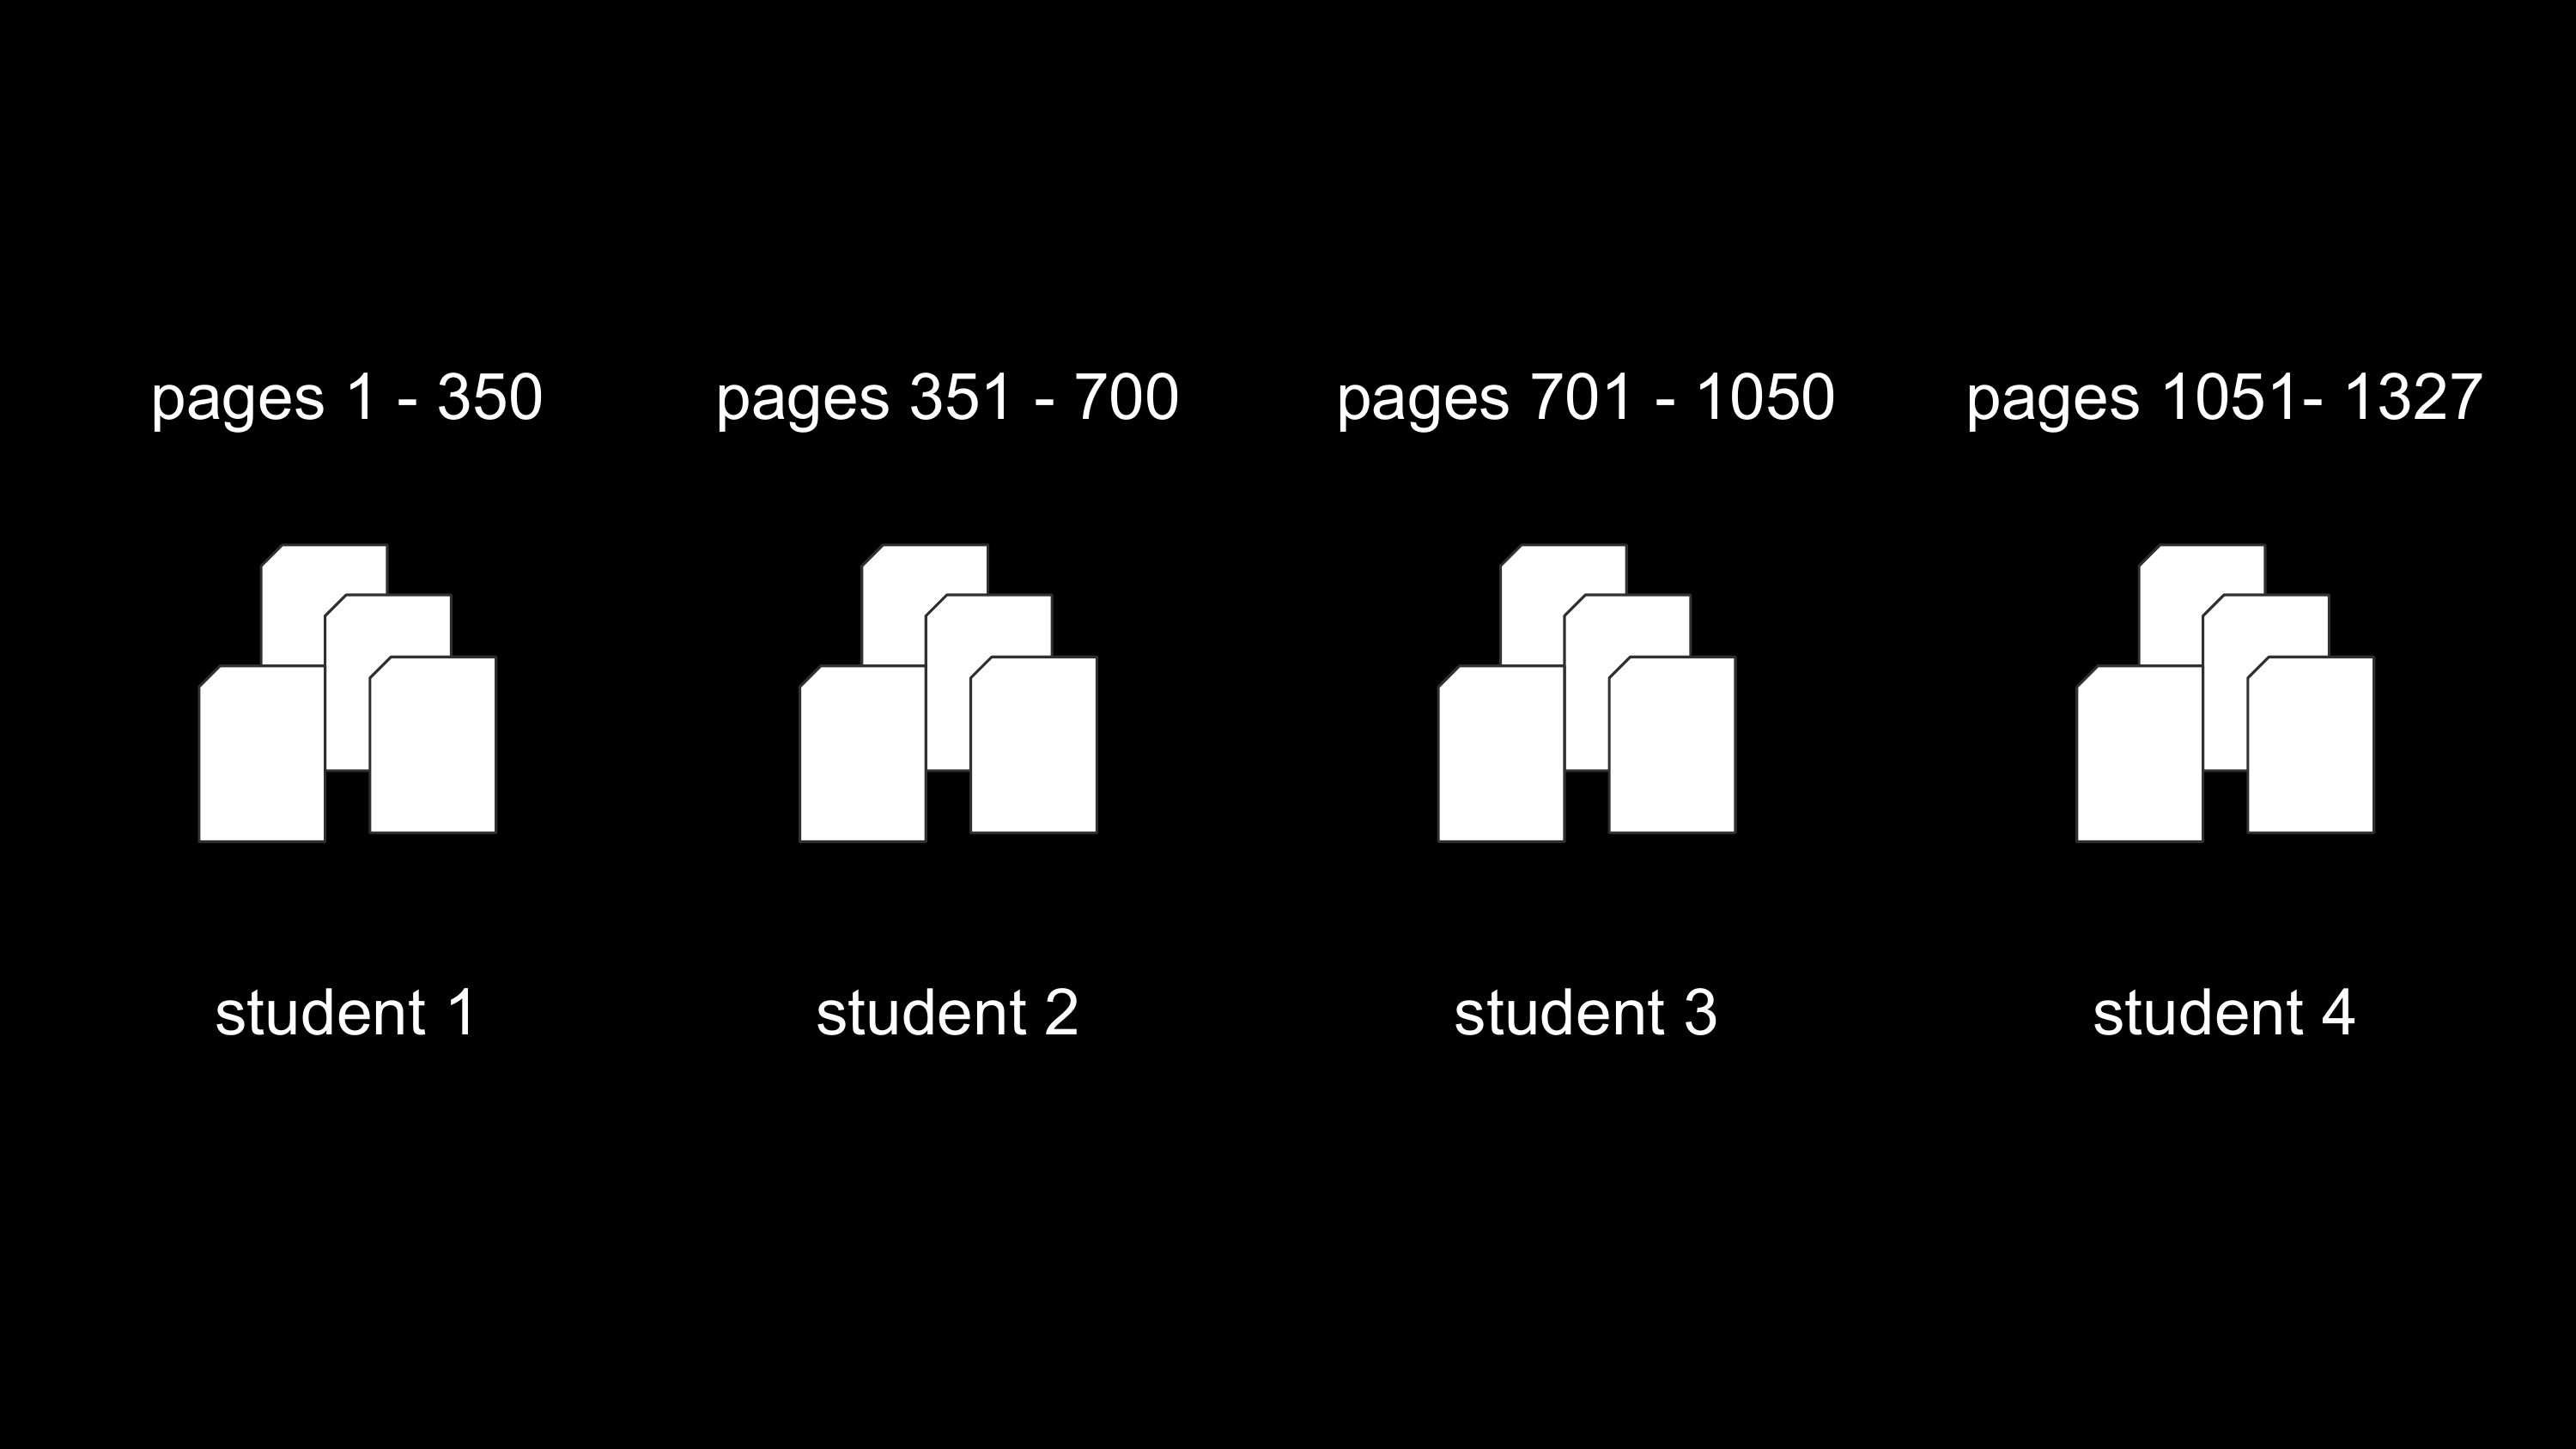
\includegraphics[width=0.6\linewidth,height=\textheight,keepaspectratio]{index_files/mediabag/problem_solving_exam12345678.png}

}

\caption{\label{fig-problem-solving-word-count-distributed}Verteiltes
Wörterzählen}

\end{figure}%

Durch die Verteilung und parallele Ausführung kann das EVA-Modell wie in
Abbildung~\ref{fig-eva-distributed} angepasst und detaillierter
dargestellt werden. Statt eines einzelnen Prozesses
\texttt{count\_words} laufen nun \(n\) parallele Prozesse, die jeweils
einen Teil des Buches durchsuchen. Die Aufteilung erfolgt zu Beginn
durch den \texttt{split}-Prozess, während das Zusammenführen der
Teilergebnisse -- in diesem Fall das Addieren der Teilsummen -- durch
den \texttt{merge}-Schritt erfolgt.

\begin{figure}

\centering{

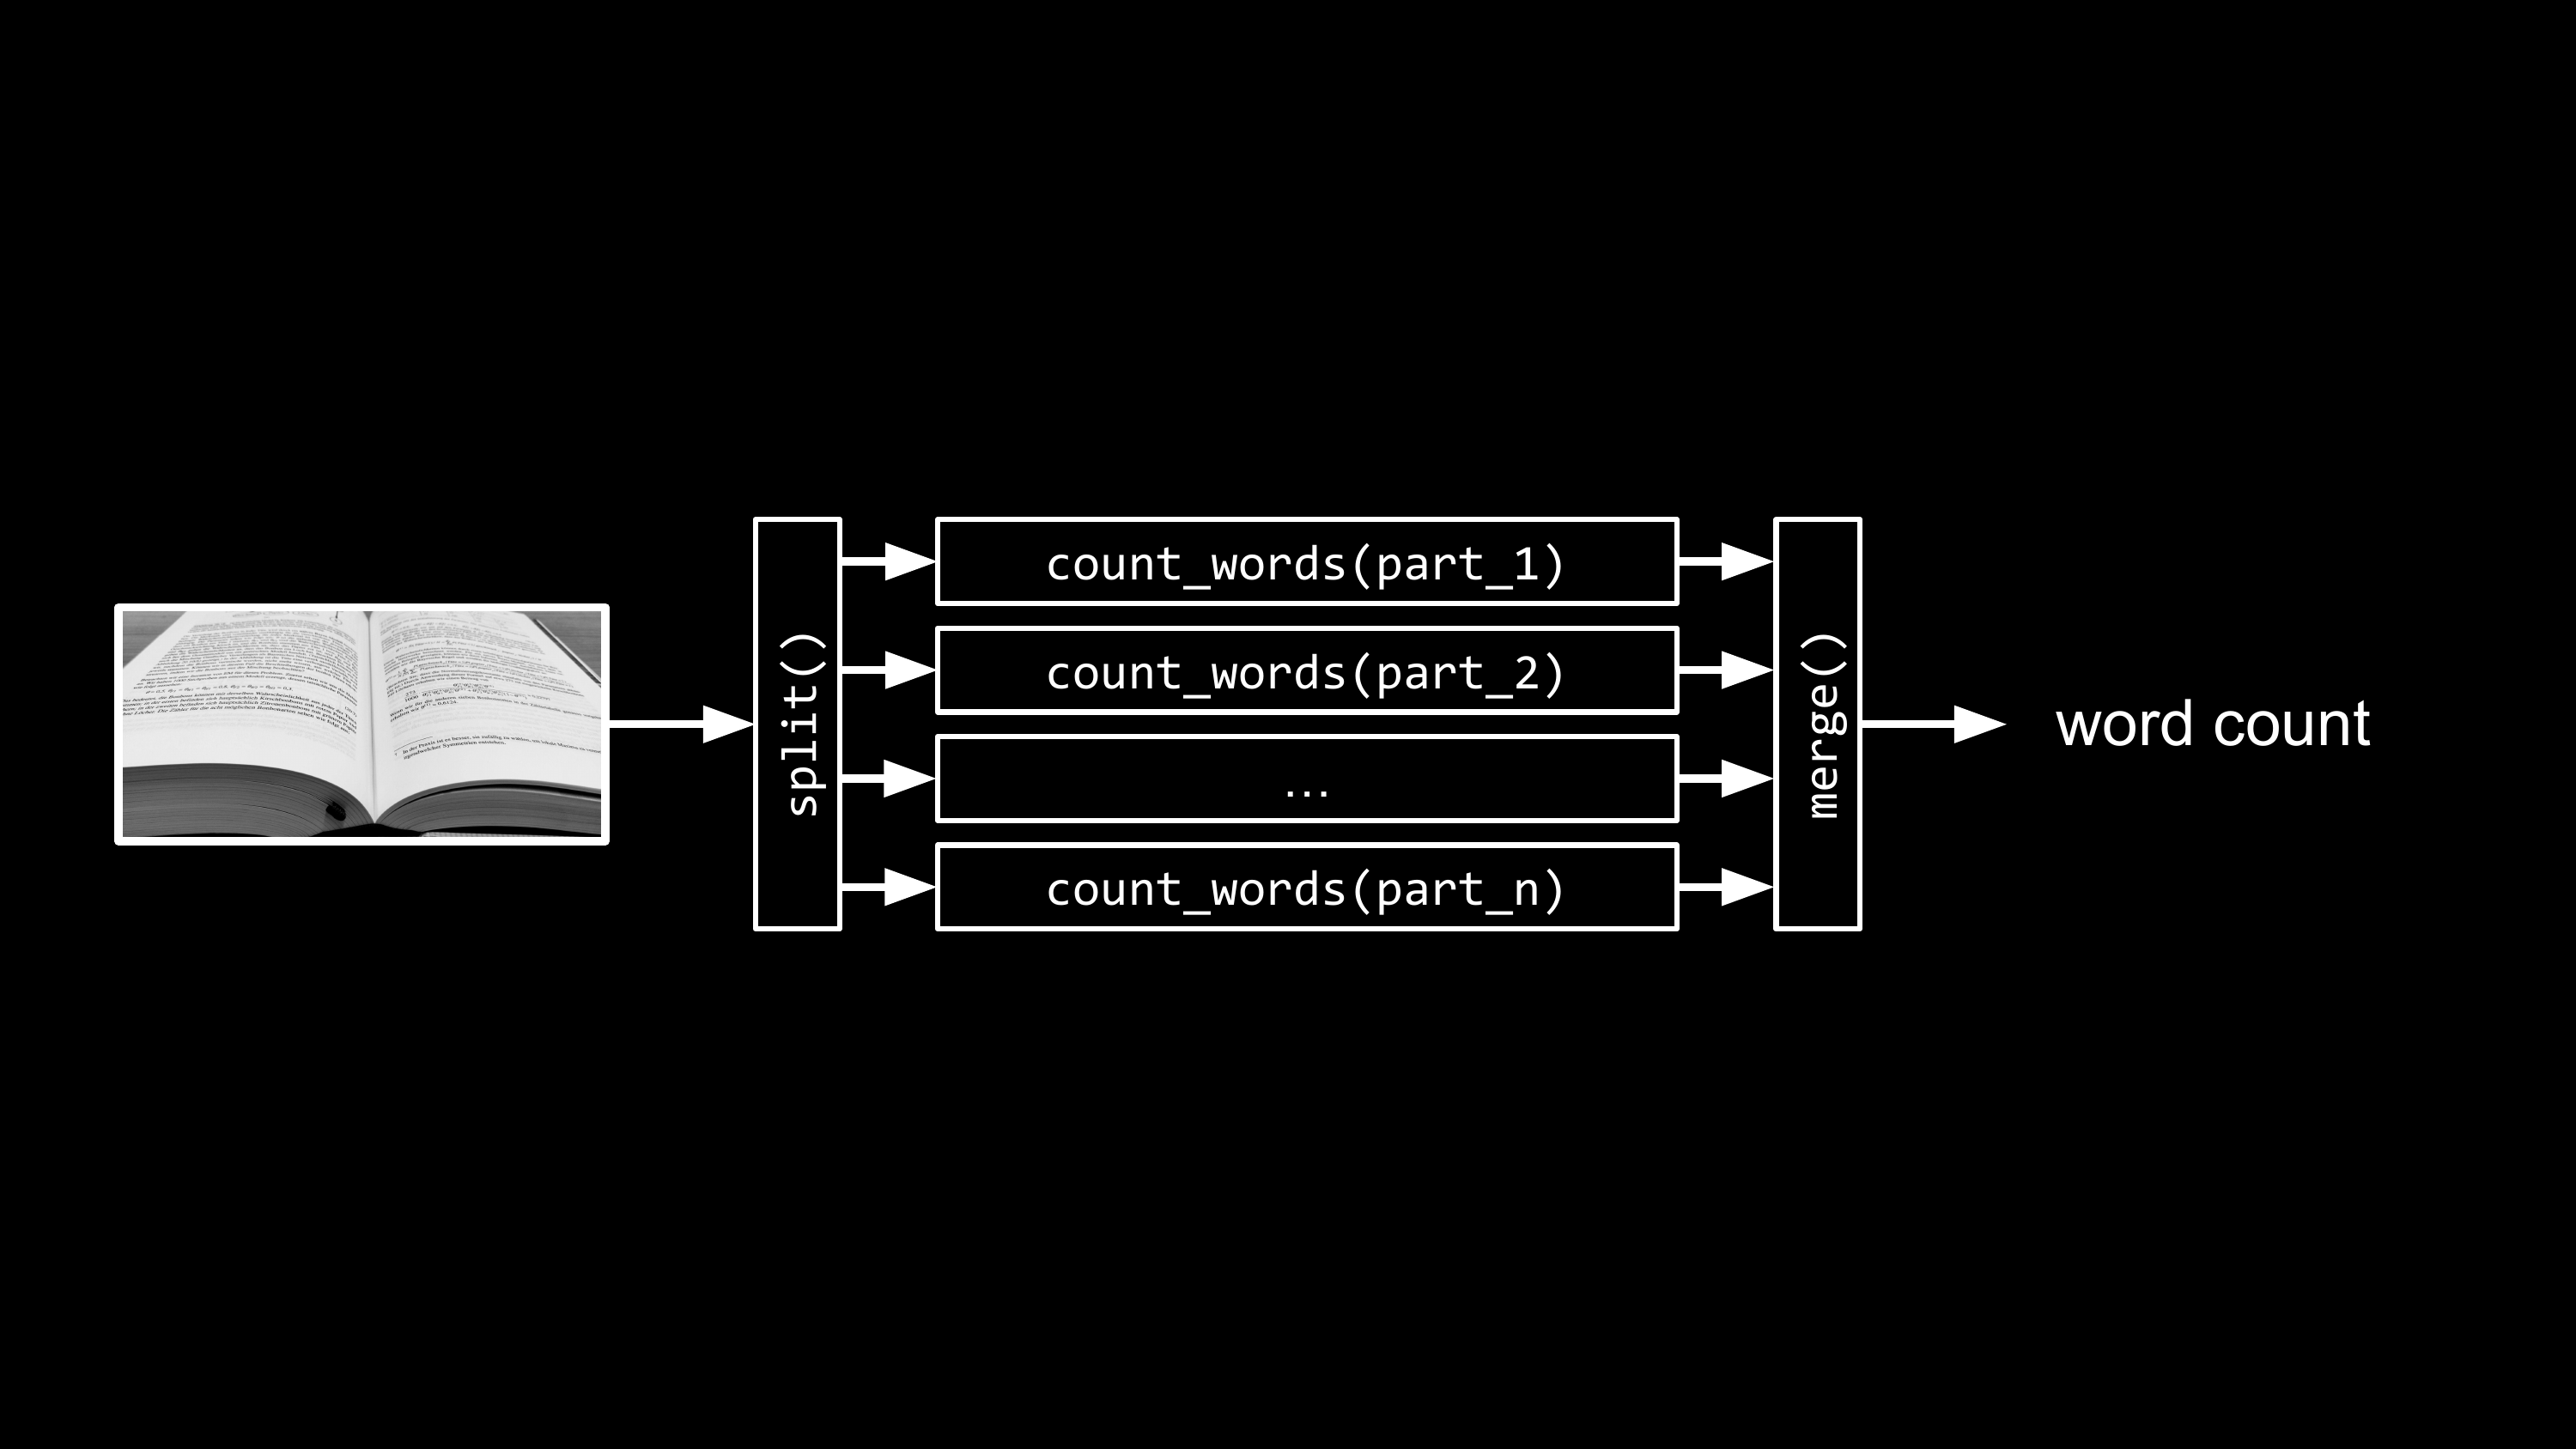
\includegraphics[width=0.6\linewidth,height=\textheight,keepaspectratio]{index_files/mediabag/problem_solving_exam123456789.png}

}

\caption{\label{fig-eva-distributed}Das parallelisierte Wörterzählen im
EVA-Modell}

\end{figure}%

In diesem Kapitel haben wir uns mit dem EVA-Modell auseinandergesetzt -
einem fundamentalen Konzept für die computergestützte Problemlösung.
Dieses Modell bietet uns einen strukturierten Rahmen, der aus drei
wesentlichen Komponenten besteht:

\begin{itemize}
\item
  \textbf{Eingabe (E)}: Die zu verarbeitenden Daten oder Informationen
\item
  \textbf{Verarbeitung (V)}: Der Kern der Problemlösung durch
  Algorithmen
\item
  \textbf{Ausgabe (A)}: Das Ergebnis der Verarbeitung in nutzbarer Form
\end{itemize}

Die Verarbeitung als zentrales Element des Modells ist dabei der Ort, an
dem die eigentliche Problemlösung stattfindet. Hier kommen Algorithmen
zum Einsatz - präzise Handlungsanweisungen, die Schritt für Schritt zur
Lösung führen. Die genaue Natur dieser Algorithmen, ihre
charakteristischen Eigenschaften und wie wir sie entwickeln können,
werden wir im nächsten Kapitel detailliert betrachten.

\chapter{Algorithmen}\label{sec-algorithms}

\section{Zusammenfassung}\label{zusammenfassung}

Willkommen zum Kapitel über Algorithmen - ein fundamentales Konzept der
Informatik und der digitalen Problemlösung. In diesem Abschnitt werden
wir uns mit den grundlegenden Aspekten von Algorithmen befassen und
dabei zentrale Fragen beantworten:

\begin{itemize}
\item
  Was ist ein Algorithmus und wie grenzt er sich von einem
  Computerprogramm ab?
\item
  Welche verschiedenen Kategorien von Algorithmen existieren und durch
  welche praktischen Beispiele lassen sie sich veranschaulichen?
\item
  Wie können wir Algorithmen systematisch und präzise formulieren?
\item
  Nach welchen Kriterien bewerten wir die Effizienz und Eignung
  verschiedener Algorithmen für spezifische Problemstellungen?
\end{itemize}

\section{Was ist ein Algorithmus?}\label{was-ist-ein-algorithmus}

\subsection{Herkunft des Begriffs}\label{herkunft-des-begriffs}

Der Begriff ``\textbf{Algorithmus}''
\href{https://www.wissenschaftsjahr.de/2008/coremedia/generator/wj2008/de/02__Mathematik__alles__was__z_C3_A4hlt/05__KW50__Algorithmus.html}{stammt
vom Namen des persischen Mathematikers Muhammad al-Khwarizmi}, der um
das Jahr 780 n.~Chr. geboren wurde. Al-Khwarizmi war ein bedeutender
Gelehrter am Hofe des Kalifen al-Mamun und verfasste dort Schriften, die
den Gebrauch der indischen Zahlzeichen erklärten. Diese Schriften wurden
im 12. Jahrhundert ins Lateinische übersetzt, wobei der Titel
``Algoritmi de numero Indorum'' verwendet wurde. Im Laufe der Zeit wurde
der Name al-Khwarizmi zur Bezeichnung für die von ihm beschriebenen
Rechenverfahren und entwickelte sich schließlich zum modernen Begriff
``Algorithmus''.

Heute bezeichnet ein \textbf{Algorithmus} eine präzise Abfolge von
Anweisungen, die ein bestimmtes Problem lösen oder eine Aufgabe erfüllen
sollen. Im Alltag begegnen uns Algorithmen ständig, oft, ohne dass wir
es merken: beim Kochen, bei der Wegbeschreibung oder beim Aufbau eines
IKEA-Regals.

\subsection{Algorithmen und Programme}\label{algorithmen-und-programme}

Ein wichtiger Aspekt von Algorithmen ist ihre Universalität: Sie sind
nicht an Computer gebunden. Ein Algorithmus ist im Kern eine
strukturierte Anleitung zur Problemlösung, unabhängig davon, wer oder
was diese Anleitung ausführt. Diese Flexibilität zeigt sich besonders
deutlich in unserem Alltag, wo wir ständig algorithmische Anleitungen
befolgen - sei es beim Aufbau eines Möbelstücks oder beim Kochen nach
einem Rezept. Bei diesen Tätigkeiten führen wir Menschen die
algorithmischen Schritte aus, ganz ohne Beteiligung eines Computers:

\begin{itemize}
\tightlist
\item
  Kochen: Ein Rezept ist ein Algorithmus für die Zubereitung eines
  Gerichts.
\end{itemize}

Comment

\begin{itemize}
\item
  Wegbeschreibung: Eine Schritt-für-Schritt-Anleitung, um von Punkt A
  nach Punkt B zu gelangen.
\item
  Bastelanleitung: Die Anweisungen, um ein Modellflugzeug
  zusammenzubauen.
\end{itemize}

Viele Algorithmen können von Computern ausgeführt werden. Dafür ist
jedoch eine Übersetzung in eine maschinenverständliche Form notwendig.
Diese Übersetzung erfolgt durch das Programmieren, wobei wir den
Algorithmus in einer Programmiersprache formulieren. Um die Beziehung
zwischen Algorithmen und Computerprogrammen besser zu verstehen, ist es
hilfreich, drei zentrale Begriffe zu unterscheiden:

\begin{itemize}
\item
  \textbf{Algorithmus}: Die abstrakte Beschreibung einer Lösungsmethode
  in Form einer präzisen, endlichen Sequenz von individuellen
  Anweisungen. Ein Algorithmus ist unabhängig von der konkreten
  Umsetzung und kann sowohl von Menschen als auch von Maschinen
  ausgeführt werden.
\item
  \textbf{Programm}: Die konkrete Implementation eines oder mehrerer
  Algorithmen in einer Programmiersprache. Das Programm übersetzt die
  abstrakten Anweisungen des Algorithmus in eine Form, die ein Computer
  verstehen und ausführen kann.
\item
  \textbf{Prozess}: Die tatsächliche Ausführung eines Programms durch
  einen Computer. Dabei werden die programmierten Anweisungen Schritt
  für Schritt abgearbeitet, um das gewünschte Ergebnis zu erzielen.
\end{itemize}

\section{Kategorien}\label{kategorien}

Algorithmen können nach ihrer Funktion und ihrem Anwendungsbereich in
verschiedene Kategorien eingeteilt werden. Jede Kategorie repräsentiert
einen spezifischen Problemlösungsansatz:

\begin{itemize}
\item
  \textbf{Mathematische Algorithmen}: Berechnen oder approximieren Werte
\item
  \textbf{Suchalgorithmen}: Finden bestimmte Elemente in einer
  Datenmenge
\item
  \textbf{Sortieralgorithmen}: Ordnen Daten nach bestimmten Kriterien
\item
  \textbf{Optimierungsalgorithmen}: Finden die bestmögliche Lösung für
  ein Problem
\item
  \textbf{Graphenalgorithmen}: Arbeiten mit vernetzten Strukturen
\item
  \textbf{Stochastische Algorithmen}: Verwenden Zufallselemente, um ein
  Problem zu lösen
\item
  \textbf{Maschinelle Lernalgorithmen}: Erkennen Muster und treffen
  Vorhersagen
\end{itemize}

Diese Kategorien sind weder vollständig noch strikt voneinander
getrennt. Viele Algorithmen lassen sich mehreren Kategorien zuordnen.
Ein anschauliches Beispiel hierfür ist der
\textbf{Dijkstra-Algorithmus}\index{Dijkstra-Algorithmus}, der die
kürzeste Route zwischen zwei Punkten findet. Er ist sowohl ein
Graphenalgorithmus, da er auf vernetzten Strukturen arbeitet, als auch
ein Optimierungsalgorithmus, da er die optimale (kürzeste) Route
ermittelt.

Im folgenden beleuchten wir ein oder mehr Beispiele für jeder der
genannten Klassen.

\subsection{Mathematische Algorithmen}\label{mathematische-algorithmen}

\subsubsection{Größter gemeinsamer Teiler
(GGT)}\label{gruxf6uxdfter-gemeinsamer-teiler-ggt}

Der Algorithmus zur Berechnung des größten gemeinsamen Teilers (GGT) ist
ein klassisches Beispiel für einen eleganten mathematischen Algorithmus.
Er wurde vom griechischen Mathematiker Euklid um 300 v. Chr. in seinem
Werk ``Die Elemente'' beschrieben und demonstriert eindrucksvoll die
zeitlose Natur algorithmischen Denkens.

Das Verfahren basiert auf einem einfachen, aber genialen Prinzip: Der
GGT zweier Zahlen ist identisch mit dem GGT der kleineren Zahl und der
Differenz beider Zahlen. Zum Beispiel haben die Zahlen 48 und 18 den
gleichen GGT wie 18 und 30 (48-18). Durch wiederholtes Anwenden dieser
Regel wird der GGT systematisch ermittelt. Die Eleganz dieses Verfahrens
liegt in seiner Einfachheit und mathematischen Präzision -
Eigenschaften, die auch heute noch moderne Algorithmen auszeichnen.

Der Block unten zeigt die Schritte des Euklidschen Algorithmus für das
obige Zahlenbeispiel.

\begin{Shaded}
\begin{Highlighting}[]
\NormalTok{Loop }\DecValTok{1}\NormalTok{:}
\NormalTok{a }\OperatorTok{=} \DecValTok{18}\NormalTok{, b }\OperatorTok{=} \DecValTok{48} 
\NormalTok{a }\OperatorTok{\textless{}}\NormalTok{ b → swap: a }\OperatorTok{=} \DecValTok{48}\NormalTok{, b }\OperatorTok{=} \DecValTok{18}
\NormalTok{a }\OperatorTok{=} \DecValTok{48} \OperatorTok{{-}} \DecValTok{18} \OperatorTok{=} \DecValTok{30}

\NormalTok{Loop }\DecValTok{2}\NormalTok{: }
\NormalTok{a }\OperatorTok{=} \DecValTok{30}\NormalTok{, b }\OperatorTok{=} \DecValTok{18} 
\NormalTok{a }\OperatorTok{\textgreater{}=}\NormalTok{ b → no swap}
\NormalTok{a }\OperatorTok{=} \DecValTok{30} \OperatorTok{{-}} \DecValTok{18} \OperatorTok{=} \DecValTok{12}

\NormalTok{Loop }\DecValTok{3}\NormalTok{: }
\NormalTok{a }\OperatorTok{=} \DecValTok{12}\NormalTok{, b }\OperatorTok{=} \DecValTok{18} 
\NormalTok{a }\OperatorTok{\textless{}}\NormalTok{ b → swap: a }\OperatorTok{=} \DecValTok{18}\NormalTok{, b }\OperatorTok{=} \DecValTok{12}
\NormalTok{a }\OperatorTok{=} \DecValTok{18} \OperatorTok{{-}} \DecValTok{12} \OperatorTok{=} \DecValTok{6}

\NormalTok{Loop }\DecValTok{4}\NormalTok{:}
\NormalTok{a }\OperatorTok{=} \DecValTok{6}\NormalTok{, b }\OperatorTok{=} \DecValTok{12} 
\NormalTok{a }\OperatorTok{\textless{}}\NormalTok{ b → swap: a }\OperatorTok{=} \DecValTok{12}\NormalTok{, b }\OperatorTok{=} \DecValTok{6}
\NormalTok{a }\OperatorTok{=} \DecValTok{12} \OperatorTok{{-}} \DecValTok{6} \OperatorTok{=} \DecValTok{6}

\NormalTok{Loop }\DecValTok{5}\NormalTok{:}
\NormalTok{a }\OperatorTok{=} \DecValTok{6}\NormalTok{, b }\OperatorTok{=} \DecValTok{6} 
\NormalTok{a }\OperatorTok{\textgreater{}=}\NormalTok{ b → no swap}
\NormalTok{a }\OperatorTok{=} \DecValTok{6} \OperatorTok{{-}} \DecValTok{6} \OperatorTok{=} \DecValTok{0}

\NormalTok{result: b }\OperatorTok{=} \DecValTok{6}
\end{Highlighting}
\end{Shaded}

\subsubsection{Babylonisches
Wurzelziehen}\label{babylonisches-wurzelziehen}

\subsection{Suchalgorithmen}\label{suchalgorithmen}

\subsubsection{Lineare Suche}\label{lineare-suche}

\subsubsection{Binäre Suche}\label{binuxe4re-suche}

\subsubsection{Suche in Bäumen}\label{suche-in-buxe4umen}

\subsection{Sortieralgorithmen}\label{sortieralgorithmen}

\subsection{Optimierungsalgorithmen}\label{optimierungsalgorithmen}

\subsubsection{Dijkstra-Algorithmus}\label{dijkstra-algorithmus}

\subsection{Graphenalgorithmen}\label{graphenalgorithmen}

\subsection{Stochastische Algorithmen}\label{stochastische-algorithmen}

\subsubsection{}\label{section}

\subsection{Maschinelle
Lernalgorithmen}\label{maschinelle-lernalgorithmen}

\section{Iteration und Rekursion}\label{iteration-und-rekursion}

\part{Repräsentation}

\chapter{Informationen}\label{sec-information}

\begin{figure}

\begin{minipage}{0.20\linewidth}
\href{https://youtu.be/g-QOJ6z0VFE}{\begin{center}
\pandocbounded{
\includegraphics[keepaspectratio]{qrcodes/g-QOJ6z0VFE.png}}
\end{center}
}\end{minipage}%
%
\begin{minipage}{0.80\linewidth}
Zu diesem Kapitel gibt es ein Video auf YouTube. Scanne einfach den
QR-Code oder klicke in der digitalen Version des Buches auf den
QR-Code.\end{minipage}%

\end{figure}%

\section{Information in der
Informatik}\label{information-in-der-informatik}

Hast du dich jemals gefragt, was eigentlich Information genau ist? Jeder
hat eine intuitive Vorstellung davon, was wir mit Information meinen.
Aber was ist die genaue Definition? Und wie ist der Begriff
\emph{Information} im Zusammenhang mit digtialen Computern gemeint?

Hier schon einmal eine Definition, die wir in diesem Kapitel anhand von
einigen Beispielen genauer verstehen wollen.

\begin{figure}[H]

{\centering \includegraphics[width=0.6\linewidth,height=\textheight,keepaspectratio]{index_files/mediabag/information_definiti.png}

}

\caption{Lauet dieser Definition erhöht Information unsere
Treffsicherheit bei Vorhersagen.}

\end{figure}%

\subsection{Zahlenraten}\label{zahlenraten}

Um der Information auf die Spur zu kommen beginnen wir mit einem
Gedankenexperiment. Stell dir vor, wir spielen ein Zahlenratespiel. Ich
denke an eine Zahl zwischen 1 und 16, und dein Ziel ist es, sie zu
erraten. Der Haken ist, dass du nur einen Versuch hast, die richtige
Zahl zu erraten, aber du kannst die Möglichkeiten vorher durch Fragen
der Form ``Ist die Zahl größer als X?'' eingrenzen. Für jede Frage werde
ich dir mit ``ja'' oder ``nein'' antworten und damit die verbleibenden
Optionen reduzieren.

Mit jeder Antwort, die du erhältst, wächst dein Wissen über meine Zahl,
was bedeutet, dass deine \textbf{Unsicherheit} bezüglich der gesuchten
Zahl abnimmt. Du kannst einige mögliche Zahlen ausschließen, wenn du
eine neue Antwort erhältst.

Wir halten zunächst fest, dass das Eingrenzen der verbleibenden
Möglichkeiten die Unsicherheit reduziert. Wir untersuchen nun, wie diese
Idee die Grundlage der Informationstheorie bildet. Durch die Reduzierung
der Unsicherheit sammeln wir mit jedem Versuch mehr
\textbf{Information}. Aber wie viel Information erhältst du mit jeder
Antwort? Und wie können wir das messen?

\begin{figure}[H]

{\centering 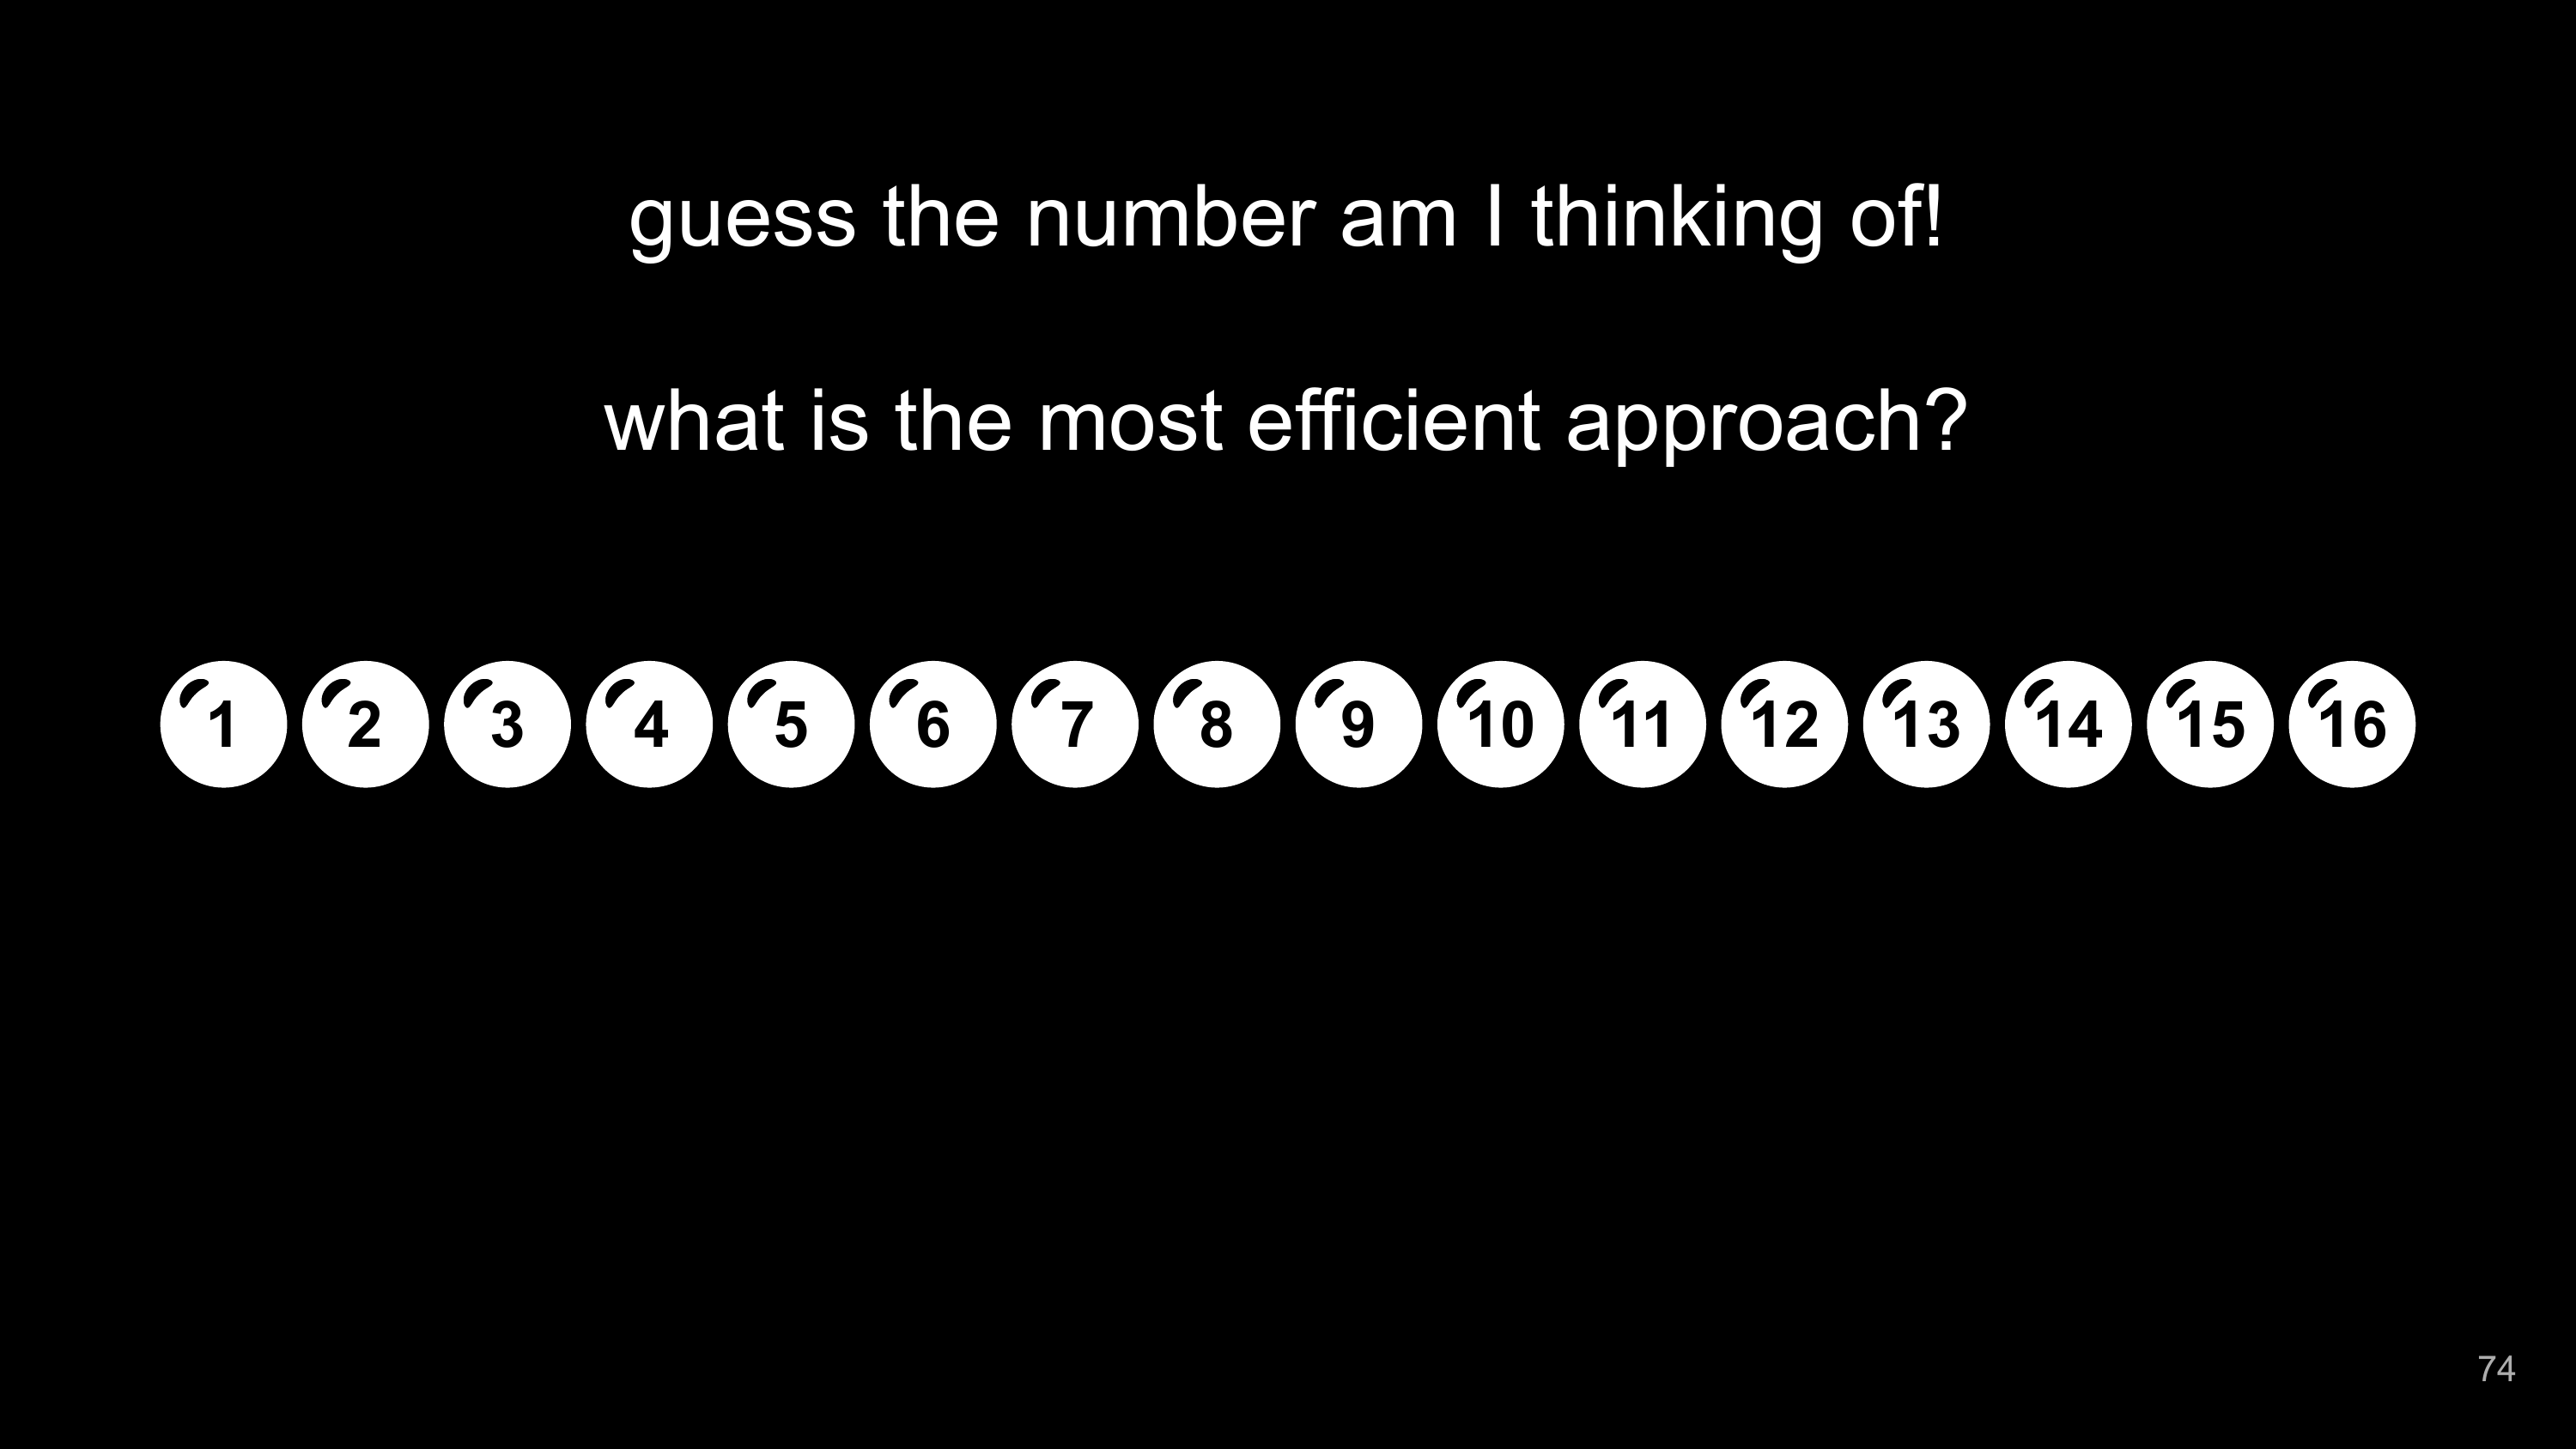
\includegraphics[width=0.6\linewidth,height=\textheight,keepaspectratio]{index_files/mediabag/number_guessing_game.png}

}

\caption{Ich denke an eine Zahl zwischen 1 und 16. Deine Aufgabe ist es,
die Zahl mit so wenig Fragen wie möglich zu erraten.}

\end{figure}%

\subsection{Bit für Bit}\label{bit-fuxfcr-bit}

In der Informatik kann Information definiert werden als ``das, was es
ermöglicht, eine korrekte Vorhersage mit besserer Genauigkeit als der
Zufall zu treffen'' {[}CITE{]}. Einfacher ausgedrückt bedeutet dies, die
Unsicherheit durch Eingrenzung der möglichen Optionen zu reduzieren.

Vor diesem Hintergrund wollen wir unser Zahlenratespiel noch einmal
genauer betrachten. Wie oben beschrieben, versuchst du meine Zahl zu
erraten, und jede Antwort, die du von mir erhältst, grenzt den Bereich
der möglichen Zahlen ein. Diese Reduzierung der Unsicherheit kann mit
einer Einheit namens \textbf{Bit} gemessen werden. Ein Bit, was für
\textbf{binary digit} (Binärziffer) steht, ist die grundlegende Einheit
der Information. Es zeigt eine Halbierung der Unsicherheit an. Einfacher
ausgedrückt: Wenn eine neue Antwort nur noch halb so viele Optionen wie
zuvor übrig lässt, liefert sie uns genau ein Bit an Information.

Allerdings werden nicht alle Fragen und deren Antworten genau ein Bit
Information liefern. Wenn zum Beispiel deine erste Frage im Ratespiel
lautet: ``Ist deine Zahl größer als 12?'' und die Antwort ``nein'' ist,
bleiben die Zahlen 1 bis 12 übrig. Das bedeutet, du hast noch 12
Optionen von ursprünglich 16, was die Unsicherheit nicht halbiert. Es
werden nur 4 statt der nötigen 8 Möglichkeiten entfernt. Lautet die
Antwort dagegen ``ja'', so kannst du insgesamt 12 Möglichkeiten
streichen, was mehr als der Hälfte entspricht und der Informationsgehalt
der Antwort wäre größer als ein Bit.

Um genau ein Bit Information zu erhalten, solltest du darauf abzielen,
mit jeder Frage genau die Hälfte der möglichen Zahlen auszuschließen.
Wenn du zum Beispiel fragst ``Ist deine Zahl größer als 8?'', stellst du
sicher, dass du - egal ob die Antwort ``ja'' oder ``nein'' ist - in
beiden Fällen 8 mögliche Zahlen übrig behältst. Ist die Antwort ``ja'',
bleiben die Zahlen 9 bis 16 übrig. Ist die Antwort ``nein'', bleiben die
Zahlen 1 bis 8. In beiden Szenarien wird deine Unsicherheit um die
Hälfte reduziert, also um ein Bit.

Indem du deine Fragen sorgfältig so wählst, dass sie die verbleibenden
Optionen jedes Mal halbieren, reduzierst du deine Unsicherheit Bit für
Bit und machst es dir leichter und schneller, die richtige Zahl zu
finden.

\begin{figure}[H]

{\centering \includegraphics[width=0.6\linewidth,height=\textheight,keepaspectratio]{index_files/mediabag/number_guessing_game1.png}

}

\caption{Deine Fragen sollten die Anzahl der Möglichkeiten halbieren.}

\end{figure}%

Angenommen, die Antwort auf deine erste Frage ``Ist deine Zahl größer
als 8?'' war ``nein''. Was sollte deine nächste Frage sein, um die
Unsicherheit weiterhin effektiv zu reduzieren? Die beste Strategie ist
es zu fragen: ``Ist sie größer als 4?''. Diese Vorgehensweise stellt
sicher, dass dir immer nur vier mögliche Zahlen bleiben: entweder 1 bis
4, wenn die Antwort ``nein'' ist, oder 5 bis 8, wenn die Antwort ``ja''
ist. Erneut halbiert dies die verbleibenden Optionen und liefert genau
ein Bit an Information.

\begin{figure}[H]

{\centering \includegraphics[width=0.6\linewidth,height=\textheight,keepaspectratio]{index_files/mediabag/number_guessing_game12.png}

}

\caption{Nach zwei Fragen bleiben noch 4 Möglichkeitn, wenn die Fragen
gut gewählt wurden.}

\end{figure}%

Lass uns mit dieser Methode fortfahren. Angenommen, deine zweite Frage
``Ist sie größer als 4?'' erhält ein ``nein'' als Antwort. Deine neue
Auswahl an Zahlen ist auf 1, 2, 3 und 4 begrenzt. Um die Unsicherheit
weiter zu reduzieren, wäre die nächste logische Frage: ``Ist sie größer
als 2?'' Dies lässt dir entweder die Zahlen 1 und 2 oder 3 und 4,
abhängig von der Antwort.

Indem du weiterhin Fragen stellst, die systematisch die verbleibenden
Optionen halbieren, kannst du sehen, wie wir schrittweise die
Unsicherheit Bit für Bit reduzieren. Schließlich wirst du nach nur vier
Fragen die Zahl auf genau eine eingrenzen, da keine anderen
Möglichkeiten mehr übrig sind. Das bedeutet, du hast die Unsicherheit
auf null reduziert.

\begin{figure}[H]

{\centering \includegraphics[width=0.6\linewidth,height=\textheight,keepaspectratio]{index_files/mediabag/number_guessing_game123.png}

}

\caption{Wir benötigen vier Ja/Nein-Fragen, um die Optionen von 16 auf
eine einzige zu reduzieren.}

\end{figure}%

\subsection{Unsicherheit}\label{unsicherheit}

Wir haben gerade gelernt, dass wir mit jeder Ja/Nein-Frage, die die
Hälfte der Möglichkeiten eliminiert, ein Bit an Information gewinnen.
Aber wie können wir dieses Konzept der Reduktion von Unsicherheit
mathematisch quantifizieren? Wir gehen das Schritt für Schritt durch.

Stell dir vor, du bist am Anfang unseres Zahlenratespiels. Es gibt 16
mögliche Zahlen, an die ich denken könnte, daher ist deine
Wahrscheinlichkeit, beim ersten Versuch die richtige Zahl zu erraten,
ziemlich gering:

\[
P_{correct} = \frac{1}{16}
\]

Das entspricht einer Wahrscheinlichkeit von nur 0,0625 - definitiv nicht
zu deinen Gunsten. Angenommen, du stellst eine Frage, die die
Möglichkeiten auf die Hälfte reduziert. Jetzt verbessert sich deine
Chance, richtig zu raten:

\[
P_{correct} = \frac{1}{8}
\]

Mit jeder weiteren Frage verdoppelt sich diese Wahrscheinlichkeit,
während sich deine Unsicherheit halbiert. Ist Wahrscheinlichkeit die
beste Methode, um Unsicherheit zu messen? Wenn wir möchten, dass unser
Maß für Unsicherheit abnimmt, während wir mehr Informationen sammeln,
ist es es sinnvoll, den Kehrwert der Wahrscheinlichkeit zu verwenden.
Das entspräche der Anzahl an Möglichkeiten, die noch im Rennen sind.

Zu Beginn gibt es 16 Möglichkeiten, also begänne die Unsicherheit bei
16. Nach der ersten Frage fiele sie auf 8, dann auf 4, 2 und schließlich
1. Allerdings würde dieses Maß uns selbst dann, wenn nur noch eine
Option übrig ist, eine gewisse Unsicherheit, nämlich 1, anzeigen, was
nicht ganz unserem intuitiven Verständnis entspricht. Wenn wir sicher
sind, dann sollte die Unsicherheit 0 sein.

Claude Shannon, der Vater der Informationstheorie, schlug einen anderen
Ansatz vor. Er empfahl, die Unsicherheit mithilfe des Logarithmus zur
Basis 2 der Anzahl der Möglichkeiten zu messen:

\[
H = log_2(N)
\]

Diese Methode hat mehrere Vorteile. Erstens ist die Unsicherheit gleich
null, wenn es nur eine mögliche Antwort gibt (N=1), was mit unserer
Intuition übereinstimmt:

\[
log_2(1) = 0
\]

Ein weiterer Vorteil ist die Einfachheit der Berechnungen, besonders
wenn es um mehrere unabhängige Unsicherheiten geht. Nehmen wir an, das
Spiel ändert sich: Jetzt denke ich an zwei unabhängige Zahlen zwischen 1
und 16. Bevor du irgendwelche Fragen stellst, beträgt deine Unsicherheit
für jede Zahl:

\[
log_2(16)= 4~bits
\]

Die Gesamtunsicherheit für beide Zahlen ist einfach die Summe ihrer
individuellen Unsicherheiten:

\[
log_2(16)+log_2(16)=8~bits
\]

Wenn wir stattdessen Wahrscheinlichkeiten verwenden, müssten wir die
Chancen multiplizieren, um die Wahrscheinlichkeit zu finden, beide
Zahlen korrekt zu erraten:

\[
P_{correct,correct}=\frac{1}{16}\times\frac{1}{16}=\frac{1}{256}
\]

Mit beiden Zahlen gibt es 256 Möglichkeiten. Mit Shannons Methode
erhalten wir das gleiche Ergebnis:

\[
log_2(256)=8~bits
\]

Wie du siehst, vereinfacht die Verwendung von Logarithmen unsere
Berechnungen, besonders wenn es um mehrere Quellen der Unsicherheit
geht. Diese Klarheit und Einfachheit sind der Grund, warum Shannons
Ansatz fundamental für die Informationstheorie geworden ist.

\subsection{Information}\label{information}

Um den Begriff \emph{Information} aus dem Begriff der
\emph{Unsicherheit} herzuleiten, betrachten wir zwei Zustände: Die
ursprüngliche Unsicherheit vor einer Frage, die wir als \(H_0\)
bezeichnen, und die reduzierte Unsicherheit nach der Antwort, die wir
\(H_1\) nennen. Die Menge an Information \(I\), die wir durch die
Antwort gewinnen, entspricht der Differenz dieser beiden Unsicherheiten:

\[
I = H_0 - H_1
\]

Information ist also die Reduzierung von Unsicherheit. Mit der obigen
Formel können wir die Information \(I\) präzise quantifizieren. Dies
ermöglicht uns zu berechnen, wie viel Information wir durch jede Frage
gewinnen. Betrachten wir ein konkretes Beispiel aus unserem
Zahlenratespiel: Angenommen, deine erste Frage ist ``Ist deine Zahl
größer als 12?'' und die Antwort lautet ``nein''. Dann bleiben die
Zahlen 1 bis 12 als Möglichkeiten übrig. Die gewonnene Information
berechnet sich wie folgt:

\[
I = log_2(16) - log_2(12) \approx 4 - 3.585 \approx 0.415~bits
\]

In diesem Fall lieferte die Antwort etwa 0,415 Bits an Information --
also weniger als ein Bit. Das ist folgerichtig, da die Antwort weniger
als die Hälfte der Möglichkeiten eliminiert hat.

Wie sähe es aus, wenn die Antwort ``ja'' gewesen wäre? In diesem Fall
blieben nur die Zahlen 13, 14, 15 und 16 übrig, also vier mögliche
Optionen:

\[
I = log_2(16) - log_2(4) = 4-2= 2~bits
\]

Diese Antwort lieferte mehr als ein Bit, nämlich 2 Bits. Wie lässt sich
dieser Unterschied erklären?

\subsection{Unwahrscheinliche
Antworten}\label{unwahrscheinliche-antworten}

Die Menge an Information hängt von der Wahrscheinlichkeit der jeweiligen
Antwort ab. Bei einer Frage, die die Möglichkeiten halbiert, hat jede
Antwort ``Ja'' oder ``Nein'' auf die Frage ``Ist die Zahl größer als
X?'' eine Wahrscheinlichkeit von genau 50\%. Diese gleichmäßige
Verteilung vereinfacht die Berechnung und liefert genau ein Bit an
Information.

Bei der Frage ``Ist deine Zahl größer als 12?'' sind die beiden
Antworten ``Ja'' und ``Nein'' allerdings nicht gleich wahrscheinlich. Es
gibt zwölf mögliche Zahlen, die ein ``Nein'' ergeben und nur vier, die
ein ``Ja'' ergeben, was Wahrscheinlichkeiten von 75\% für ``Nein'' und
25\% für ``Ja'' bedeutet. Da die ``Ja''-Antwort weniger wahrscheinlich
ist, ist sie überraschender -- und liefert deshalb mehr Information. Wie
wir berechnet haben, gibt uns ein ``Ja'' 2 Bits an Information, während
ein ``Nein'' nur 0,415 Bits liefert.

Dieser Zusammenhang ist ein Kernprinzip der Informationstheorie: Je
unwahrscheinlicher ein Ereignis ist, desto mehr Information enthält sein
Auftreten. Umgekehrt liefert eine sehr wahrscheinliche Antwort, wie das
``Nein'' im obigen Beispiel, weniger Information, da sie weniger
überraschend ist.

Warum zielen wir darauf ab, Fragen zu stellen, die die Möglichkeiten
gleichmäßig halbieren? Man könnte auch wild raten in der Hoffnung, durch
eine unwahrscheinlichere Antwort mehr Informationen zu bekommen -- auch
wenn man seltener richtig liegt. Die Antwort ist einfach: Eine Frage,
die den Raum der Möglichkeiten halbiert, maximiert unseren
\emph{erwarteten} Informationsgewinn. Zwar können wir mit einer
riskanten Frage wie ``Ist die Zahl größer 15?'' unser Glück
herausfordern und im Erfolgsfall die Unsicherheit stark verringern. Dies
ist jedoch keine nachhaltige Strategie. Wenn wir das Spiel nicht nur
einmal, sondern 10, 100 oder 1000 Mal spielen, nähern wir uns im Mittel
dem Erwartungswert für die gewonnene Information \(E[I]\). Und dieser
Erwartungswert favorisiert eindeutig Fragen, die die Hälfte der
Möglichkeiten eliminieren.

Um dies zu verdeutlichen, berechnen wir zunächst den Erwartungswert für
die extreme Frage ``Ist die Zahl größer 15?'':

\[
E[I] = \left( \frac{1}{16}\times 4 \right)+ \left(\frac{15}{16}\times 0.09311 \right)= 0.3373
\]

Der Erwartungswert berechnet sich durch den mit der Wahrscheinlichkeit
gewichteten Informationsgewinn für jede mögliche Antwort. Bei der Frage
``Ist die Zahl größer als 15?'' gibt es ein ``Ja'' nur dann, wenn die
Zahl 16 ist. Von den sechzehn möglichen Zahlen erzeugt also nur eine
diese Antwort. Die Wahrscheinlichkeit beträgt somit \(\frac{1}{16}\). In
diesem Fall reduziert sich unsere Unsicherheit sofort auf Null, da nur
noch eine einzige Möglichkeit übrig bleibt. Die ursprüngliche
Unsicherheit betrug 4 Bits:

\[
H_0 = log_2(16) = 4~bits
\]

Und wenn die Unsicherheit nach der Antwort ``Ja'' auf Null reduziert
wird:

\[
H_1 = log_2(1) = 0~bits
\]

Daraus ergibt sich ein Informationsgehalt von 4 Bits:

\[
I = H_0 - H_1 = 4 - 0 = 4~bits
\]

Dies erklärt den ersten Teil der Erwartungswertgleichung. Der zweite
Teil folgt demselben Prinzip, allerdings mit einem wichtigen
Unterschied: Die Wahrscheinlichkeit für die Antwort ``Nein'' ist mit
\(\frac{15}{16}\) deutlich höher. Gleichzeitig verbleibt eine große
Restunsicherheit \(H_1\), da wir lediglich eine einzige Zahl
ausschließen konnten:

\[
H_1 = log_2(15) \approx 3.9069~bits
\]

Die gewonnene Information ist somit sehr klein:

\[
I = 4 - 3.9069 \approx 0.0931~bits
\]

Anhand der Erwartungswertformel konnten wir zeigen, dass eine extreme
Frage, die mit viel Glück direkt zum Ziel führt, in unserem Ratespiel
einen erwarteten Informationsgehalt von etwa einem Drittel Bit (0,3373)
hat. Prüfen wir nun, ob der Erwartungswert für Fragen, die die Hälfte
der Möglichkeiten eliminieren, tatsächlich höher ist:

\[
E[I] = \left(0.5 \times 1 \right) + \left(0.5 \times 1 \right) = 0.5 + 0.5 = 1~bit
\]

Wie erwartet beträgt der Erwartungswert genau 1 Bit, da bei jeder
Antwort -- ob ``Ja'' oder ``Nein'' -- jeweils die Hälfte der Optionen
eliminiert wird.

\subsection{Mehr als zwei Antworten}\label{mehr-als-zwei-antworten}

Bisher haben wir in unserem Zahlenratespiel nur Fragen mit zwei
Antwortmöglichkeiten betrachtet. Informationen, also Antworten auf
Fragen, können jedoch vielfältiger sein. Wie berechnen wir die
Information, wenn es mehr als zwei Antwortmöglichkeiten gibt?

Als Beispiel betrachten wir eine Urne mit farbigen Kugeln in drei
Farben: Rot, Grün und Blau. Aus dieser Urne ziehen wir zwei Kugeln,
wobei wir nach jedem Zug die gezogene Kugel zurück in die Urne legen.
Dieses statistische Experiment bezeichnet man als ``Ziehen mit
Zurücklegen''.

\section{Daten repräsentieren
Information}\label{daten-repruxe4sentieren-information}

\chapter{Bits}\label{bits}

\begin{figure}

\begin{minipage}{0.20\linewidth}
\href{https://www.youtube.com/watch?v=c46UqfuWJOk}{\begin{center}
\pandocbounded{
\includegraphics[keepaspectratio]{qrcodes/c46UqfuWJOk.png}}
\end{center}
}\end{minipage}%
%
\begin{minipage}{0.80\linewidth}
Zu diesem Kapitel gibt es ein Video auf YouTube. Scanne einfach den
QR-Code oder klicke in der digitalen Version des Buches auf den
QR-Code.\end{minipage}%

\end{figure}%

\section{Ist das Bit die kleinste
Informationseinheit?}\label{ist-das-bit-die-kleinste-informationseinheit}

\section{Was ist ein Byte}\label{was-ist-ein-byte}

\chapter{Codesysteme}\label{codesysteme}

\section{ASCII-Code}\label{ascii-code}

\section{Verallgemeinerung von
Codesystemen}\label{verallgemeinerung-von-codesystemen}

\section{Unicode}\label{unicode}

\section{RGB-Code}\label{rgb-code}

\section{Code vs Codec}\label{code-vs-codec}

Der Begriff \emph{Codec} leitet sich von den zwei Wörtern
en\textbf{co}der und \textbf{dec}oder ab. Die beiden Begriffe werden
zwar ähnlich geschrieben, unterscheiden sich aber in ihrer Bedeutung.
Ein Codec beschreibt ein Vorgehen oder einen Algorithmus, um Daten vor
dem Senden nach einem definierten Verfahren zu kodieren und nach dem
Empfang wieder zu dekodieren. Dies ist besonders sinnvoll, um
Informationen effizienter zu übertragen und weniger Bandbreite zu
beanspruchen. Zudem können Daten verschlüsselt und die Kommunikation
dadurch sicherer gemacht werden. Wir lernen einige Methoden für beide
Anwendungsfälle in einem späteren Kapitel kennen. Im Gegensatz dazu
beschreibt ein Code ein System, das einer Reihe von Symbolen eine
bestimmte Bedeutung zuordnet, wie wir in diesem Abschnitt gesehen haben.

\chapter{Datenstrukturen}\label{datenstrukturen}

\section{Listen}\label{listen}

\section{Mengen}\label{mengen}

\section{Graphen}\label{graphen}

\section{Bäume}\label{buxe4ume}

\section{Warteschlangen}\label{warteschlangen}

\part{Verarbeitung}

\chapter{Analog vs.~Digital}\label{analog-vs.-digital}

\begin{figure}

\begin{minipage}{0.20\linewidth}
\href{https://youtu.be/iKHU2Uj4Lp0}{\begin{center}
\pandocbounded{
\includegraphics[keepaspectratio]{qrcodes/iKHU2Uj4Lp0.png}}
\end{center}
}\end{minipage}%
%
\begin{minipage}{0.80\linewidth}
Zu diesem Kapitel gibt es ein Video auf YouTube. Scanne einfach den
QR-Code oder klicke in der digitalen Version des Buches auf den
QR-Code.\end{minipage}%

\end{figure}%

\section{Was ist der Unterschied zwischen der analogen und digitalen
Welt?}\label{was-ist-der-unterschied-zwischen-der-analogen-und-digitalen-welt}

\subsection{Endlich viele Möglichkeiten
vs.~Unendlichkeit}\label{endlich-viele-muxf6glichkeiten-vs.-unendlichkeit}

\subsection{Diskrete und kontinuierliche
Werte}\label{diskrete-und-kontinuierliche-werte}

\chapter{Speicher}\label{speicher}

\section{Substratunabhängigkeit}\label{substratunabhuxe4ngigkeit}

\chapter{Logik und Arithmetik}\label{logik-und-arithmetik}

\section{Schalter}\label{schalter}

\subsection{Relais, Vakuumröhren und
Transistoren}\label{relais-vakuumruxf6hren-und-transistoren}

\section{Logikgatter}\label{logikgatter}

\section{Binäre Addition}\label{binuxe4re-addition}

\section{Binäre Subtraktion}\label{binuxe4re-subtraktion}

\section{Substratunabhängigkeit}\label{substratunabhuxe4ngigkeit-1}

\chapter{Computer}\label{computer}

\section{Komponenten eines Computers}\label{komponenten-eines-computers}

\begin{itemize}
\tightlist
\item
  von Neumann-Architektur
\end{itemize}

\part{Kommunikation}

\chapter{Signale}\label{signale}

\section{Was ist ein Signal?}\label{was-ist-ein-signal}

``A signal is a function that conveys information about the behavior of
a system or attributes of some phenomenon''.

Ein Signal ist eine physikalische Größe, die Informationen trägt.
Stellen wir uns vor, du stehst an einer Straßenecke und winkst einem
Freund auf der anderen Seite zu. Deine Handbewegung ist
ein~\textbf{optisches Signal}, das die Information „Komm her!{}``
überträgt. Signale können auch Schallwellen (wie deine Stimme),
elektrische Impulse (in Kabeln) oder Licht (in Glasfasern) sein

\subsection{Der Kern ist die
Veränderung}\label{der-kern-ist-die-veruxe4nderung}

Eine statische physikalische Größe kann keine Informationen übertragen.
Dies haben wir bereits im Kapitel Kapitel~\ref{sec-information}
kennengelernt. Erst die Veränderung einer physikalischen Größe über die
Zeit ermöglicht es, Informationen zu kodieren und zu übertragen. Ein
einfaches Beispiel ist das An- und Ausschalten einer Lampe, wobei die
Veränderung der Helligkeit das Signal darstellt. Die zeitliche Abfolge
dieser Veränderungen kann dann als Nachricht interpretiert werden, wie
etwa beim Morsecode.

\subsection{Häufig elektrisch}\label{huxe4ufig-elektrisch}

Ein Signal muss nicht unbedingt eine elektrische Größe wie Spannung
(gemessen in Volt) sein. Signale können auch mechanische Größen (Druck,
Beschleunigung), optische Größen (Helligkeit, Farbe) oder akustische
Größen (Schallwellen) sein. Das Entscheidende ist, dass sich das Signal
als messbare Größe über die Zeit verändert und dadurch Informationen
transportiert.

Für die Verarbeitung mit Computern müssen wir alle Signale in
elektrische Signale umwandeln. Von dort aus ist es dann ein kleiner
Schritt zum digitalen Signal, das nur die Werte Null oder Eins annehmen
kann. Dafür nutzen wir sogenannte \textbf{Analog-to-Digital-Converter
(ADC)}.

\section{Wie können wir Signale
erzeugen?}\label{wie-kuxf6nnen-wir-signale-erzeugen}

\subsection{Von digital zu analog}\label{von-digital-zu-analog}

\subsection{Die LED}\label{die-led}

\section{Wie können wir Signale
emfpangen?}\label{wie-kuxf6nnen-wir-signale-emfpangen}

\subsection{Von analog zu digital}\label{von-analog-zu-digital}

\subsection{Der Farbsensor}\label{der-farbsensor}

\section{Welche Bedeutung hat ein
Signal?}\label{welche-bedeutung-hat-ein-signal}

Ein Signal ist zunächst nur eine messbare Abfolge von Veränderungen
einer physikalischen Größe über die Zeit. Die Bedeutung, die wir diesen
Veränderungen -- oder der Modulation -- zuschreiben, bestimmen wir
selbst.

\chapter{Protokolle}\label{protokolle}

\section{Peer-To-Peer}\label{peer-to-peer}

\section{Handshake}\label{handshake}

\section{TCP/IP \& HTTPs}\label{tcpip-https}

\begin{itemize}
\item
  How can we communicate between two computers?

  \begin{itemize}
  \item
    Protocols / Handshake
  \item
    Netzwerk / Internet / P2P-Communication
  \end{itemize}
\end{itemize}

\chapter{Verschlüsselung}\label{verschluxfcsselung}

\section{Verschlüsselung}\label{verschluxfcsselung-1}

\subsection{Symmetrisch}\label{symmetrisch}

\begin{itemize}
\tightlist
\item
  Symmetric encryption with Caesar Cipher
\end{itemize}

\subsection{Asymmetrisch}\label{asymmetrisch}

\begin{itemize}
\tightlist
\item
  Assymetric with RSA Toy
\end{itemize}

\section{Digitale Signaturen}\label{digitale-signaturen}

\begin{itemize}
\tightlist
\item
  Digital signatures
\end{itemize}

\chapter{Kompression}\label{kompression}

\section{Verlustfreie Kompression}\label{verlustfreie-kompression}

\begin{itemize}
\tightlist
\item
  Huffman
\end{itemize}

\section{Verlustbehaftete
Kompression}\label{verlustbehaftete-kompression}

\begin{itemize}
\tightlist
\item
  JPEG
\end{itemize}

\bookmarksetup{startatroot}

\chapter*{Literaturverzeichnis}\label{literaturverzeichnis}
\addcontentsline{toc}{chapter}{Literaturverzeichnis}

\markboth{Literaturverzeichnis}{Literaturverzeichnis}

\phantomsection\label{refs}
\begin{CSLReferences}{1}{0}
\bibitem[\citeproctext]{ref-adami_what_2016}
Adami, Christoph. 2016. {„What is {Information}?``} \emph{Philosophical
Transactions of the Royal Society A: Mathematical, Physical and
Engineering Sciences} 374 (2063): 20150230.
\url{https://doi.org/10.1098/rsta.2015.0230}.

\bibitem[\citeproctext]{ref-brookshear_computer_2020}
Brookshear, J. Glenn, und Dennis Brylow. 2020. \emph{Computer science:
an overview}. 13th edition, global edition. NY, NY: Pearson.

\bibitem[\citeproctext]{ref-petzold_code_2022}
Petzold, Charles. 2022. \emph{Code: the hidden language of computer
hardware and software}. 2. Aufl. Hoboken: Microsoft Press.

\bibitem[\citeproctext]{ref-UBHD-66395843}
Pólya, George, und John Horton Conway. 2004. \emph{How to solve it: a
new aspect of mathematical method}. Expanded Princeton Science Library
ed. Princeton science library. Princeton {[}N.J.{]}: Princeton
University Press.

\bibitem[\citeproctext]{ref-scott_but_2009}
Scott, John C. 2009. \emph{But how do it know?: the basic principles of
computers for everyone}. Oldsmar, FL: John C. Scott.

\end{CSLReferences}



\printindex


\end{document}
